\section{Building the model}
\label{sec:application:building_the_model}

Within this section, the 15 steps are provided to build the model represented by \cref{fig:application:the_model:final_ecore_model}. For each of these 15 steps, the corresponding Ecore model and GROOVE graphs are shown.

Before the model is built, it is necessary to initialize the initial models. The initial models are empty and are used as a starting point. Each step will then add more elements to the model until the final model is obtained. Therefore, define the following models:

\begin{tabularx}{\textwidth}{|lX|}
\hline
\multicolumn{2}{|l|}{\textbf{Initial models}}\\
\hhline{|==|}
$Tm_0 = $ & $Tm_\epsilon$ (\cref{defin:transformation_framework:type_models_and_type_graphs:combining_type_models:empty_type_model}) \\
$Im_0 = $ & $Im_\epsilon$ (\cref{defin:transformation_framework:instance_models_and_instance_graphs:combining_instance_models:empty_instance_model})\\
\hline
$TG_0 = $ & $TG_\epsilon$ (\cref{defin:transformation_framework:type_models_and_type_graphs:combining_type_graphs:empty_type_graph})\\
$IG_0 = $ & $IG_\epsilon$ (\cref{defin:transformation_framework:instance_models_and_instance_graphs:combining_instance_graphs:empty_instance_graph})\\
\hline
$f_0(Im_0) = $ & $IG_\epsilon$ (\cref{defin:transformation_framework:instance_models_and_instance_graphs:combining_instance_graphs:empty_instance_graph})\\
$f'_0(IG_0) = $ & $Im_\epsilon$ (\cref{defin:transformation_framework:instance_models_and_instance_graphs:combining_instance_models:empty_instance_model})\\
\hline
\end{tabularx}

Essentially, every model is defined to be the empty model, and every graph is defined to be the empty graph. Furthermore, $f_0$ is the mapping function which projects $Im_0$ (and $Tm_0$) onto $IG_0$ (and $TG_0$). $f'_0$ is the inverse function which maps $IG_0$ (and $TG_0$) onto $Im_0$ (and $Tm_0$).

\subsection{Houses}
\label{subsec:application:building_the_model:houses}

The first step of building the model is to add a type. Without any types, nothing interesting can be produced. The first type will be the class type for houses. \cref{subsec:library_of_transformations:type_level_transformations:regular_classes} is used to introduce the class type, while on the instance level, \cref{subsec:library_of_transformations:instance_level_transformations:plain_objects} is used to introduce the house objects.

The $name$ of the new house type is $.\type{House}$. Furthermore, 2 house objects are introduced, $objects = \{TR, BHP\}$. Furthermore, we assume that the object identifiers are equal to the internal node id, so $fid(TR) = TR$ and $fid(BHP) = BHP$. The following model is obtained:

\LTXtable{\textwidth}{tex/06_application/02_building_the_model/tables/01_houses.tex}

\begin{figure}[p]
    \centering
    \begin{subfigure}{0.98\textwidth}
        \centering
        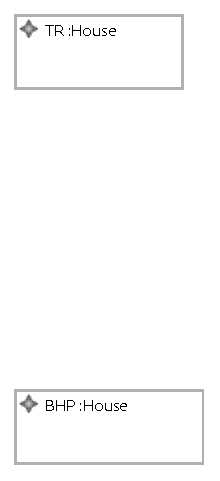
\includegraphics{images/06_application/instance_model/step01.pdf}
        \caption{Instance Model $Im_1$}
        \label{fig:application:building_the_model:houses:ecore:instance_model}
    \end{subfigure}
    \\
    \begin{subfigure}{0.98\textwidth}
        \centering
        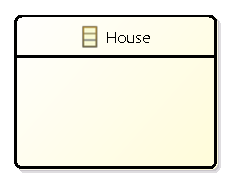
\includegraphics{images/06_application/type_model/step01.pdf}
        \caption{Type Model $Tm_1$}
        \label{fig:application:building_the_model:houses:ecore:type_model}
    \end{subfigure}
    \caption{The Ecore model after step 1}
    \label{fig:application:building_the_model:houses:ecore}
\end{figure}

\begin{figure}[p]
    \centering
    \begin{subfigure}{0.98\textwidth}
        \centering
        % To use this figure in your LaTeX document
% import the package groove/resources/groove2tikz.sty
%
\begin{tikzpicture}[scale=\tikzscale,name prefix=step01-]
\node[type_node] (n0) at (0.530, -0.370) {\ml{\textbf{House}}};

\end{tikzpicture}

        \caption{Instance Graph $IG_1$}
        \label{fig:application:building_the_model:houses:groove:instance_graph}
    \end{subfigure}
    \\
    \begin{subfigure}{0.98\textwidth}
        \centering
        % To use this figure in your LaTeX document
% import the package groove/resources/groove2tikz.sty
%
\begin{tikzpicture}[scale=\tikzscale,name prefix=step01-]
\node[type_node] (n0) at (0.530, -0.370) {\ml{\textbf{House}}};

\end{tikzpicture}

        \caption{Type Graph $TG_1$}
        \label{fig:application:building_the_model:houses:groove:type_graph}
    \end{subfigure}
    \caption{The GROOVE graphs after step 1}
    \label{fig:application:building_the_model:houses:groove}
\end{figure}

A visual representation of $Tm_1$ and $Im_1$ can be found in \cref{fig:application:building_the_model:houses:ecore}. Similarly, a visual representation of $TG_1$ and $IG_1$ can be found in \cref{fig:application:building_the_model:houses:groove}. Please note that because of the definitions of $f_1(Im_1)$ and $f'_1(IG_1)$, we have that $f_1(Im_1) = IG_1$ and $f'_1(IG_1) = Im_1$. Furthermore, $f_1(Im_1)$ and $f'_1(IG_1)$ are valid mapping functions themselves, such that they can be combined with another mapping function in the next step.

The models itself are not very special as of yet, but that is expected. Each step is only a small building block, and introducing a type is not very special.

\afterpage{\FloatBarrier}
\begin{longtable}{|lX|}
\hline
\multicolumn{2}{|l|}{\textbf{Models after step 2}}\\
\hhline{|==|}
\endhead
$Tm_2 = $ & $\mathrm{combine}(Tm_1, Tm_{Class}) =$ \newline
$\begin{aligned}
Class =\ & \{.\type{House}, .\type{Room}\} \\
Enum =\ & \{\} \\
UserDataType =\ & \{\} \\
Field =\ & \{\} \\
\mathrm{FieldSig} =\ & \{\} \\
EnumValue =\ & \{\} \\
Inh =\ & \{\} \\
Prop =\ & \{\} \\
Constant =\ & \{\} \\
\mathrm{ConstType} =\ & \{\}
\end{aligned}$
\\
$Im_2 = $ & $\mathrm{combine}(Tm_1, Im_{Class}) =$ \newline
$\begin{aligned}
Object =\ &\{TR, BHP\} \\
\mathrm{ObjectClass}(ob) =\ & \{(TR, .\type{House}), (BHP, .\type{House})\}\\
\mathrm{ObjectId} =\ & \{(TR, TR), (BHP, BHP)\}\\
\mathrm{FieldValue} =\ & \{\} \\
\mathrm{DefaultValue} =\ & \{\}
\end{aligned}$
\\
\hline
$TG_2 = $ & $\mathrm{combine}(TG_1, TG_{Class}) =$ \newline
$\begin{aligned}
NT =\ & \{\langle \type{House} \rangle, \langle \type{Room} \rangle\} \\
ET =\ & \{\} \\
\!\!\sqsubseteq\ =\ & \big\{
\big(\langle \type{House} \rangle, \langle \type{House} \rangle \big),
\big(\langle \type{Room} \rangle, \langle \type{Room} \rangle \big)
\big\} \\
abs =\ & \{\} \\
\mathrm{mult} =\ & \{\} \\
contains =\ & \{\}
\end{aligned}$
\\
$IG_2 = $ & $\mathrm{combine}(TG_1, IG_{Class}) =$ \newline
$\begin{aligned}
N =\ & \{TR, BHP\} \\
E =\ & \{\} \\
\mathrm{ident} =\ & \{(TR, TR), (BHP, BHP)\} \\
\mathrm{type}_n =\ & \{(TR, \langle \type{House} \rangle), (BHP, \langle \type{House} \rangle)\}
\end{aligned}$
\\
\hline
$f_2(Im_2) = $ & $f_1(Im_1) \sqcup f_{Class}(Im_{Class})$ (\cref{defin:transformation_framework:instance_models_and_instance_graphs:combining_transformation_functions:combination_transformation_function_instance_model_instance_graph})\\
$f'_2(IG_2) = $ & $f'_1(IG_1) \sqcup f'_{Class}(IG_{Class})$ (\cref{defin:transformation_framework:instance_models_and_instance_graphs:combining_transformation_functions:combination_transformation_function_instance_graph_instance_model})\\
\hline
\end{longtable}
\begin{longtable}{|lX|}
\hline
\multicolumn{2}{|l|}{\textbf{Models after step 3}}\\
\hhline{|==|}
\endhead
$Tm_3 = $ & $\mathrm{combine}(Tm_2, Tm_{DataField}) =$ \newline
$\begin{aligned}
Class =\ & \{.\type{House}, .\type{Room}\} \\
Enum =\ & \{\} \\
UserDataType =\ & \{\} \\
Field =\ & \{(.\type{House}, \type{name})\} \\
\mathrm{FieldSig} =\ & \big\{\big((.\type{House}, \type{name}), (\type{string}, 1..1)\big)\big\} \\
EnumValue =\ & \{\} \\
Inh =\ & \{\} \\
Prop =\ & \{\} \\
Constant =\ & \{\} \\
\mathrm{ConstType} =\ & \{\}
\end{aligned}$
\\
$Im_3 = $ & $\mathrm{combine}(Tm_2, Im_{DataField}) =$ \newline
$\begin{aligned}
Object =\ &\{TR, BHP\} \\
\mathrm{ObjectClass}(ob) =\ & \{(TR, .\type{House}), (BHP, .\type{House})\}\\
\mathrm{ObjectId} =\ & \{(TR, TR), (BHP, BHP)\}\\
\mathrm{FieldValue} =\ & \Big\{
\Big(\big(TR, (.\type{House}, \type{name})\big), \big[\type{string}, \text{``TwoRem''}\big]\Big),\\&
\Big(\big(BHP, (.\type{House}, \type{name})\big), \big[\type{string}, \text{``B.H. Paleis''}\big]\Big)
\Big\} \\
\mathrm{DefaultValue} =\ & \{\}
\end{aligned}$
\\
\hline
$TG_3 = $ & $\mathrm{combine}(TG_2, TG_{DataField}) =$ \newline
$\begin{aligned}
NT =\ & \{\langle \type{House} \rangle, \langle \type{Room} \rangle, \type{string}\} \\
ET =\ & \big\{
\big(\langle \type{House} \rangle, \langle \type{name} \rangle, \type{string} \big)
\big\} \\
\!\!\sqsubseteq\ =\ & \big\{
\big(\langle \type{House} \rangle, \langle \type{House} \rangle \big),
\big(\langle \type{Room} \rangle, \langle \type{Room} \rangle \big),
\big(\type{string}, \type{string} \big)
\big\} \\
abs =\ & \{\} \\
\mathrm{mult} =\ & \Big\{
\Big(\big(\langle \type{House} \rangle, \langle \type{name} \rangle, \type{string} \big), \big(0..\mstar, 1..1\big) \Big)
\Big\} \\
contains =\ & \{\}
\end{aligned}$
\\
$IG_3 = $ & $\mathrm{combine}(TG_2, IG_{DataField}) =$ \newline
$\begin{aligned}
N =\ & \{TR, BHP, \text{``TwoRem''}, \text{``B.H. Paleis''}\} \\
E =\ & \Big\{
\Big(TR, \big(\langle \type{House} \rangle, \langle \type{name} \rangle, \type{string} \big), \text{``TwoRem''} \Big),\\&
\Big(BHP, \big(\langle \type{House} \rangle, \langle \type{name} \rangle, \type{string} \big), \text{``B.H. Paleis''} \Big)
\Big\} \\
\mathrm{ident} =\ & \{(TR, TR), (BHP, BHP)\} \\
\mathrm{type}_n =\ & \{
(TR, \langle \type{House} \rangle), 
(BHP, \langle \type{House} \rangle),
(\text{``TwoRem''}, \type{string}),
(\text{``B.H. Paleis''}, \type{string})
\}
\end{aligned}$
\\
\hline
$f_3(Im_3) = $ & $f_2(Im_2) \sqcup f_{DataField}(Im_{DataField})$ (\cref{defin:transformation_framework:instance_models_and_instance_graphs:combining_transformation_functions:combination_transformation_function_instance_model_instance_graph})\\
$f'_3(IG_3) = $ & $f'_2(IG_2) \sqcup f'_{DataField}(IG_{DataField})$ (\cref{defin:transformation_framework:instance_models_and_instance_graphs:combining_transformation_functions:combination_transformation_function_instance_graph_instance_model})\\
\hline
\end{longtable}
\subsection{Rooms}
\label{subsec:application:building_the_model:rooms}

In the fourth step, the room objects will be introduced as part of the introduction of the rooms containment relation. This step introduces the $\type{rooms}$ relation on the $.\type{House}$ class, including its values. \cref{subsec:library_of_transformations:type_level_transformations:contained_class_set_fields} is used to introduce the field, while on the instance level, \cref{subsec:library_of_transformations:instance_level_transformations:contained_class_set_field_values} is used to introduce the values.

The $classtype$ of the new field is $.\type{House}$, as the field will be defined for houses. The $name$ of the new field is $\type{rooms}$ and the $containedtype$ is $.\type{Room}$. The set of objects of which the value is set is equal to all house objects, so $objects = \{TR, BHP\}$. The function for $obids$ returns the existing identifier of each of these objects. The multiplicity is set to $0..9$ for the new field, and the $values$ function is defined as follows:
\begin{equation*}
    values = \big\{\big(TR, \{TRRoom1, TRRoom2\}\big), \big(BHP, \{BHPRoomA, BHPRoomB, BHPRoomC\}\big)\big\}
\end{equation*}

Please note that the referenced objects are all new. For these new objects $obids$ returns as identifier the internal node label, just as was done for the houses. The following model is obtained:

\LTXtable{\textwidth}{tex/06_application/02_building_the_model/tables/04_rooms.tex}

\begin{figure}[p]
    \centering
    \begin{subfigure}{0.98\textwidth}
        \centering
        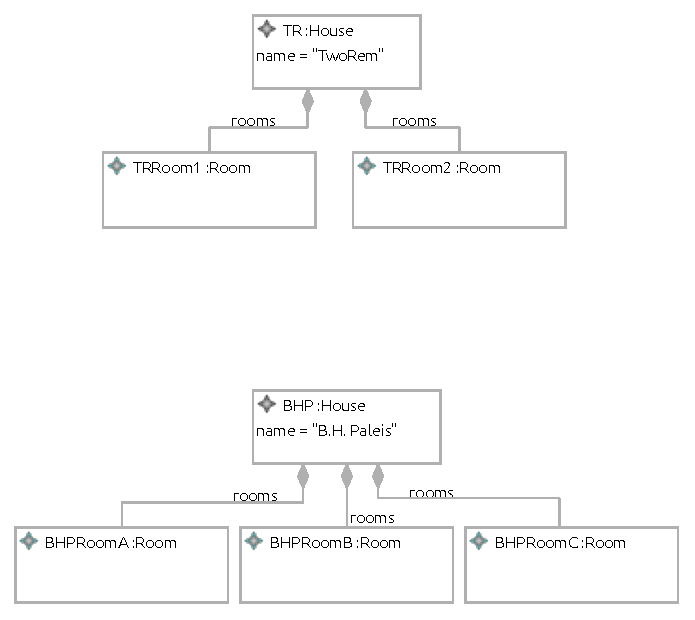
\includegraphics{images/06_application/instance_model/step04.pdf}
        \caption{Instance Model $Im_4$}
        \label{fig:application:building_the_model:rooms:ecore:instance_model}
    \end{subfigure}
    \\
    \begin{subfigure}{0.98\textwidth}
        \centering
        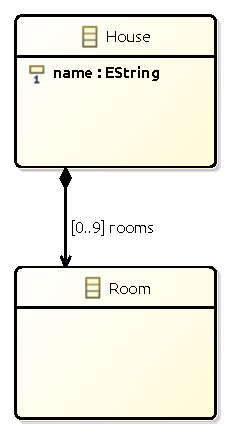
\includegraphics{images/06_application/type_model/step04.pdf}
        \caption{Type Model $Tm_4$}
        \label{fig:application:building_the_model:rooms:ecore:type_model}
    \end{subfigure}
    \caption{The Ecore model after step 4}
    \label{fig:application:building_the_model:rooms:ecore}
\end{figure}

\begin{figure}[p]
    \centering
    \begin{subfigure}{0.98\textwidth}
        \centering
        % To use this figure in your LaTeX document
% import the package groove/resources/groove2tikz.sty
%
\begin{tikzpicture}[scale=\tikzscale,name prefix=step04-]
\node[basic_node] (n0) at (2.740, -4.200) {\ml{\uline{\textit{BHP}} : \textbf{House}\\name = "B.H. Paleis"}};
\node[basic_node] (n1) at (2.660, -0.340) {\ml{\uline{\textit{TR}} : \textbf{House}\\name = "TwoRem"}};
\node[basic_node] (n7) at (1.820, -1.470) {\ml{\uline{\textit{TRRoom1}} : \textbf{Room}}};
\node[basic_node] (n8) at (3.410, -1.480) {\ml{\uline{\textit{TRRoom2}} : \textbf{Room}}};
\node[basic_node] (n14) at (0.820, -3.060) {\ml{\uline{\textit{BHPRoomA}} : \textbf{Room}}};
\node[basic_node] (n15) at (2.780, -3.050) {\ml{\uline{\textit{BHPRoomB}} : \textbf{Room}}};
\node[basic_node] (n16) at (4.720, -3.060) {\ml{\uline{\textit{BHPRoomC}} : \textbf{Room}}};

\path[basic_edge] (n0)  --  (n14) 
node[lab] at (1.584, -3.455) {\ml{rooms}};
\path[basic_edge](n0.north -| 2.780, -3.050) -- node[lab] {\ml{rooms}} (n15) ;
\path[basic_edge] (n0)  -- node[lab] {\ml{rooms}} (n16) ;
\path[basic_edge] (n1)  -- node[lab] {\ml{rooms}} (n7) ;
\path[basic_edge] (n1)  -- node[lab] {\ml{rooms}} (n8) ;
\end{tikzpicture}

        \caption{Instance Graph $IG_4$}
        \label{fig:application:building_the_model:rooms:groove:instance_graph}
    \end{subfigure}
    \\
    \begin{subfigure}{0.98\textwidth}
        \centering
        % To use this figure in your LaTeX document
% import the package groove/resources/groove2tikz.sty
%
\begin{tikzpicture}[scale=\tikzscale,name prefix=step04-]
\node[basic_node] (n0) at (2.740, -4.200) {\ml{\uline{\textit{BHP}} : \textbf{House}\\name = "B.H. Paleis"}};
\node[basic_node] (n1) at (2.660, -0.340) {\ml{\uline{\textit{TR}} : \textbf{House}\\name = "TwoRem"}};
\node[basic_node] (n7) at (1.820, -1.470) {\ml{\uline{\textit{TRRoom1}} : \textbf{Room}}};
\node[basic_node] (n8) at (3.410, -1.480) {\ml{\uline{\textit{TRRoom2}} : \textbf{Room}}};
\node[basic_node] (n14) at (0.820, -3.060) {\ml{\uline{\textit{BHPRoomA}} : \textbf{Room}}};
\node[basic_node] (n15) at (2.780, -3.050) {\ml{\uline{\textit{BHPRoomB}} : \textbf{Room}}};
\node[basic_node] (n16) at (4.720, -3.060) {\ml{\uline{\textit{BHPRoomC}} : \textbf{Room}}};

\path[basic_edge] (n0)  --  (n14) 
node[lab] at (1.584, -3.455) {\ml{rooms}};
\path[basic_edge](n0.north -| 2.780, -3.050) -- node[lab] {\ml{rooms}} (n15) ;
\path[basic_edge] (n0)  -- node[lab] {\ml{rooms}} (n16) ;
\path[basic_edge] (n1)  -- node[lab] {\ml{rooms}} (n7) ;
\path[basic_edge] (n1)  -- node[lab] {\ml{rooms}} (n8) ;
\end{tikzpicture}

        \caption{Type Graph $TG_4$}
        \label{fig:application:building_the_model:rooms:groove:type_graph}
    \end{subfigure}
    \caption{The GROOVE graphs after step 4}
    \label{fig:application:building_the_model:rooms:groove}
\end{figure}

A visual representation of $Tm_4$ and $Im_4$ can be found in \cref{fig:application:building_the_model:rooms:ecore}. Similarly, a visual representation of $TG_4$ and $IG_4$ can be found in \cref{fig:application:building_the_model:rooms:groove}. Please note that because of the definitions of $f_4(Im_4)$ and $f'_4(IG_4)$, we have that $f_4(Im_4) = IG_4$ and $f'_4(IG_4) = Im_4$. Furthermore, $f_4(Im_4)$ and $f'_4(IG_4)$ are valid mapping functions themselves, such that they can be combined with another mapping function in the next step.

The introduction of the room objects makes that the model represents something. A house has rooms that it contains, and each house has a different set of rooms. Still, there is room to enlarge the model more, such that more details are included.

\afterpage{\FloatBarrier}
\subsection{Room identifiers}
\label{sec:application:building_the_model:room_identifiers}

In the fifth step, the room identifiers are introduced by introducing another $\type{string}$ field. This step introduces gives each room a size, or in model terms, the $\type{room\_size}$ attribute on the $.\type{Room}$ class is introduced, including its values. \cref{subsec:library_of_transformations:type_level_transformations:enum_fields} is used to introduce the field on the type level, while on the instance level, \cref{subsec:library_of_transformations:instance_level_transformations:enum_field_values} is used to introduce the values.

The $classtype$ of the new field is $.\type{Room}$, as the field will be defined for rooms. The $name$ of the new field is $\type{room\_\!id}$ and the $fieldtype$ is $.\type{string}$. The set of objects of which the value is set is equal to all room objects, so $objects = \{TRRoom1, TRRoom2, BHPRoomA, BHPRoomB, BHPRoomC\}$. The function for $obids$ returns the existing identifier of each of these objects. The $values$ function is defined as follows:
\begin{align*}
    values = \{&(TRRoom1, \text{``1''}), (TRRoom2, \text{``2''}), (BHPRoomA, \text{``A''}), \\&(BHPRoomB, \text{``B''}), (BHPRoomC, \text{``C''})\}
\end{align*}

The following model is obtained:

\LTXtable{\textwidth}{tex/06_application/02_building_the_model/tables/05_room_identifiers.tex}

\begin{figure}[p]
    \centering
    \begin{subfigure}{0.98\textwidth}
        \centering
        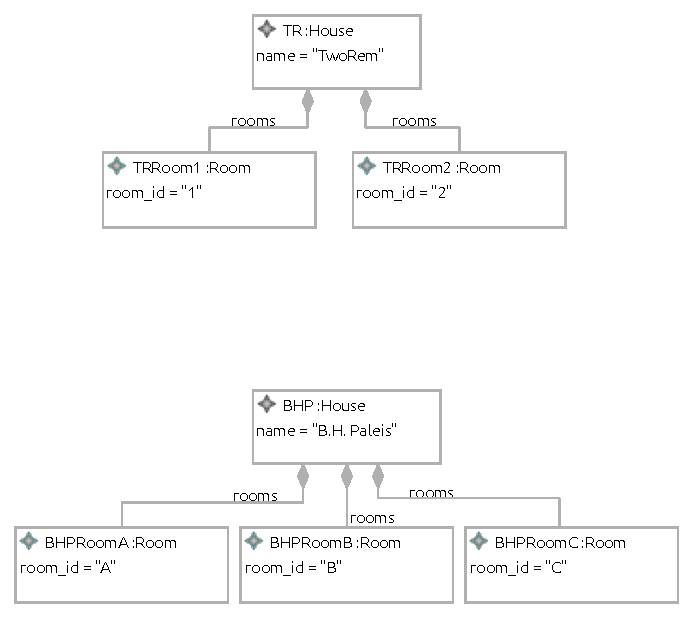
\includegraphics{images/06_application/instance_model/step05.pdf}
        \caption{Instance Model $Im_5$}
        \label{fig:application:building_the_model:room_identifiers:ecore:instance_model}
    \end{subfigure}
    \\
    \begin{subfigure}{0.98\textwidth}
        \centering
        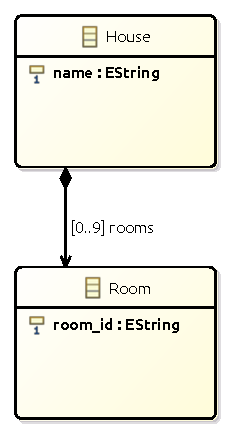
\includegraphics{images/06_application/type_model/step05.pdf}
        \caption{Type Model $Tm_5$}
        \label{fig:application:building_the_model:room_identifiers:ecore:type_model}
    \end{subfigure}
    \caption{The Ecore model after step 5}
    \label{fig:application:building_the_model:room_identifiers:ecore}
\end{figure}

\begin{figure}[p]
    \centering
    \begin{subfigure}{0.98\textwidth}
        \centering
        % To use this figure in your LaTeX document
% import the package groove/resources/groove2tikz.sty
%
\begin{tikzpicture}[scale=\tikzscale,name prefix=step05-]
\node[type_node] (n0) at (0.740, -0.400) {\ml{\textbf{House}\\name: \textbf{string}}};
\node[type_node] (n1) at (0.730, -1.585) {\ml{\textbf{Room}\\room\_id: \textbf{string}}};

\path[basic_edge, composite](n0.south -| 0.730, -1.585) -- node[lab] {\ml{rooms}} (n1) ;
\end{tikzpicture}

        \caption{Instance Graph $IG_5$}
        \label{fig:application:building_the_model:room_identifiers:groove:instance_graph}
    \end{subfigure}
    \\
    \begin{subfigure}{0.98\textwidth}
        \centering
        % To use this figure in your LaTeX document
% import the package groove/resources/groove2tikz.sty
%
\begin{tikzpicture}[scale=\tikzscale,name prefix=step05-]
\node[type_node] (n0) at (0.740, -0.400) {\ml{\textbf{House}\\name: \textbf{string}}};
\node[type_node] (n1) at (0.730, -1.585) {\ml{\textbf{Room}\\room\_id: \textbf{string}}};

\path[basic_edge, composite](n0.south -| 0.730, -1.585) -- node[lab] {\ml{rooms}} (n1) ;
\end{tikzpicture}

        \caption{Type Graph $TG_5$}
        \label{fig:application:building_the_model:room_identifiers:groove:type_graph}
    \end{subfigure}
    \caption{The GROOVE graphs after step 5}
    \label{fig:application:building_the_model:room_identifiers:groove}
\end{figure}

A visual representation of $Tm_5$ and $Im_5$ can be found in \cref{fig:application:building_the_model:room_identifiers:ecore}. Similarly, a visual representation of $TG_5$ and $IG_5$ can be found in \cref{fig:application:building_the_model:room_identifiers:groove}. Please note that because of the definitions of $f_5(Im_5)$ and $f'_5(IG_5)$, we have that $f_5(Im_5) = IG_5$ and $f'_5(IG_5) = Im_5$. Furthermore, $f_5(Im_5)$ and $f'_5(IG_5)$ are valid mapping functions themselves, such that they can be combined with another mapping function in the next step.

The visualisation unveils no surprising details. A string field was already added earlier to the house objects and introducing such a field on the room only shows that it is indeed possible to introduce fields on contained objects.

\afterpage{\FloatBarrier}
\begin{longtable}{|lX|}
\hline
\multicolumn{2}{|l|}{\textbf{Models after step 6}}\\
\hhline{|==|}
\endhead
$Tm_6 = $ & $\mathrm{combine}(Tm_5, Tm_{Enum}) =$ \newline
$\begin{aligned}
Class =\ & \{.\type{House}, .\type{Room}\} \\
Enum =\ & \{.\type{RoomSize}\} \\
UserDataType =\ & \{\} \\
Field =\ & \{(.\type{House}, \type{name}), (.\type{House}, \type{rooms}), (.\type{Room}, \type{room\_\!id})\} \\
\mathrm{FieldSig} =\ & \big\{
\big((.\type{House}, \type{name}), (\type{string}, 1..1)\big),\\&
\big((.\type{House}, \type{rooms}), ([\type{setof}, !.\type{Room}], 0..9)\big),\\&
\big((.\type{Room}, \type{room\_\!id}), (\type{string}, 1..1)\big)
\big\} \\
EnumValue =\ & \{(.\type{RoomSize}, \type{SMALL}), (.\type{RoomSize}, \type{MEDIUM}), (.\type{RoomSize}, \type{LARGE})\} \\
Inh =\ & \{\} \\
Prop =\ & \big\{\big(\type{containment}, (.\type{House}, \type{rooms})\big)\big\} \\
Constant =\ & \{\} \\
\mathrm{ConstType} =\ & \{\}
\end{aligned}$
\\
$Im_6 = $ & $\mathrm{combine}(Tm_5, Im_{Enum}) =$ \newline
$\begin{aligned}
Object =\ &\{TR, BHP, TRRoom1, TRRoom2, BHPRoomA, BHPRoomB, \\& BHPRoomC\} \\
\mathrm{ObjectClass}(ob) =\ & \{(TR, .\type{House}), (BHP, .\type{House}),
(TRRoom1, .\type{Room}),\\& (TRRoom2, .\type{Room}), (BHPRoomA, .\type{Room}), (BHPRoomB, .\type{Room}),\\& (BHPRoomC, .\type{Room})\}\\
\mathrm{ObjectId} =\ & \{(TR, TR), (BHP, BHP), (TRRoom1, TRRoom1),\\& (TRRoom2, TRRoom2), (BHPRoomA, BHPRoomA),\\& (BHPRoomB, BHPRoomB), (BHPRoomC, BHPRoomC)\}\\
\mathrm{FieldValue} =\ & \Big\{
\Big(\big(TR, (.\type{House}, \type{name})\big), \big[\type{string}, \text{``TwoRem''}\big]\Big),\\&
\Big(\big(BHP, (.\type{House}, \type{name})\big), \big[\type{string}, \text{``B.H. Paleis''}\big]\Big),\\&
\Big(\big(TR, (.\type{House}, \type{rooms})\big), \big[\type{setof}, \big\langle [\type{obj}, TRRoom1], \\&\qquad [\type{obj}, TRRoom2] \big\rangle \big]\Big),\\&
\Big(\big(BHP, (.\type{House}, \type{rooms})\big) \big[\type{setof}, \big\langle [\type{obj},  BHPRoomA], \\&\qquad [\type{obj}, BHPRoomB], (\type{obj}, BHPRoomC) \big\rangle \big]\Big),\\&
\Big(\big(TRRoom1, (.\type{Room}, \type{room\_\!id})\big), \big[\type{string}, \text{``1''}\big]\Big),\\&
\Big(\big(TRRoom2, (.\type{Room}, \type{room\_\!id})\big), \big[\type{string}, \text{``2''}\big]\Big),\\&
\Big(\big(BHPRoomA, (.\type{Room}, \type{room\_\!id})\big), \big[\type{string}, \text{``A''}\big]\Big),\\&
\Big(\big(BHPRoomB, (.\type{Room}, \type{room\_\!id})\big), \big[\type{string}, \text{``B''}\big]\Big),\\&
\Big(\big(BHPRoomC, (.\type{Room}, \type{room\_\!id})\big), \big[\type{string}, \text{``C''}\big]\Big)
\Big\} \\
\mathrm{DefaultValue} =\ & \{\}
\end{aligned}$
\\
\hline
$TG_6 = $ & $\mathrm{combine}(TG_5, TG_{EnumFlags}) =$ \newline
$\begin{aligned}
NT =\ & \{\langle \type{House} \rangle, \langle \type{Room} \rangle, \langle \type{RoomSize} \rangle, \type{string}\} \\
ET =\ & \big\{
\big(\langle \type{House} \rangle, \langle \type{name} \rangle, \type{string} \big),
\big(\langle \type{House} \rangle, \langle \type{rooms} \rangle, \langle \type{Room} \rangle \big),\\&
\big(\langle \type{Room} \rangle, \langle \type{room\_\!id} \rangle, \type{string} \big),
\big(\langle \type{RoomSize} \rangle, \langle \type{SMALL} \rangle, \langle \type{RoomSize} \rangle \big),\\&
\big(\langle \type{RoomSize} \rangle, \langle \type{MEDIUM} \rangle, \langle \type{RoomSize} \rangle \big),
\big(\langle \type{RoomSize} \rangle, \langle \type{LARGE} \rangle, \langle \type{RoomSize} \rangle \big)
\big\} \\
\!\!\sqsubseteq\ =\ & \big\{
\big(\langle \type{House} \rangle, \langle \type{House} \rangle \big),
\big(\langle \type{Room} \rangle, \langle \type{Room} \rangle \big),
\big(\langle \type{RoomSize} \rangle, \langle \type{RoomSize} \rangle \big),\\&
\big(\type{string}, \type{string} \big)
\big\} \\
abs =\ & \{\} \\
\mathrm{mult} =\ & \Big\{
\Big(\big(\langle \type{House} \rangle, \langle \type{name} \rangle, \type{string} \big), \big(0..\mstar, 1..1\big) \Big),\\&
\Big(\big(\langle \type{House} \rangle, \langle \type{rooms} \rangle, \langle \type{Room} \rangle \big), \big(0..1, 0..9\big) \Big),\\&
\Big(\big(\langle \type{Room} \rangle, \langle \type{room\_\!id} \rangle, \type{string} \big), \big(0..\mstar, 1..1\big) \Big),\\&
\Big(\big(\langle \type{RoomSize} \rangle, \langle \type{SMALL} \rangle, \langle \type{RoomSize} \rangle \big), \big(0..1, 0..1\big) \Big),\\&
\Big(\big(\langle \type{RoomSize} \rangle, \langle \type{MEDIUM} \rangle, \langle \type{RoomSize} \rangle \big), \big(0..1, 0..1\big) \Big),\\&
\Big(\big(\langle \type{RoomSize} \rangle, \langle \type{LARGE} \rangle, \langle \type{RoomSize} \rangle \big), \big(0..1, 0..1\big) \Big)
\Big\} \\
contains =\ & \big\{\big(\langle \type{House} \rangle, \langle \type{rooms} \rangle, \langle \type{Room} \rangle \big)\big\}
\end{aligned}$
\\
$IG_6 = $ & $\mathrm{combine}(TG_5, IG_{EnumFlags}) =$ \newline
$\begin{aligned}
N =\ & \{TR, BHP, TRRoom1, TRRoom2, BHPRoomA, BHPRoomB, BHPRoomC, \\& 
SmallSize, MediumSize, LargeSize,
\text{``TwoRem''}, \text{``B.H. Paleis''}, \text{``1''},  \text{``2''}, \text{``A''}, \text{``B''},\\& \text{``C''}\} \\
E =\ & \Big\{
\Big(TR, \big(\langle \type{House} \rangle, \langle \type{name} \rangle, \type{string} \big), \text{``TwoRem''} \Big),\\&
\Big(BHP, \big(\langle \type{House} \rangle, \langle \type{name} \rangle, \type{string} \big), \text{``B.H. Paleis''} \Big),\\&
\Big(TR, \big(\langle \type{House} \rangle, \langle \type{rooms} \rangle, \langle \type{Room} \rangle \big), TRRoom1 \Big),\\&
\Big(TR, \big(\langle \type{House} \rangle, \langle \type{rooms} \rangle, \langle \type{Room} \rangle \big), TRRoom2 \Big),\\&
\Big(BHP, \big(\langle \type{House} \rangle, \langle \type{rooms} \rangle, \langle \type{Room} \rangle \big), BHPRoomA \Big),\\&
\Big(BHP, \big(\langle \type{House} \rangle, \langle \type{rooms} \rangle, \langle \type{Room} \rangle \big), BHPRoomB \Big),\\&
\Big(BHP, \big(\langle \type{House} \rangle, \langle \type{rooms} \rangle, \langle \type{Room} \rangle \big), BHPRoomC \Big),\\&
\Big(TRRoom1, \big(\langle \type{Room} \rangle, \langle \type{room\_\!id} \rangle, \type{string} \big), \text{``1''} \Big),\\&
\Big(TRRoom2, \big(\langle \type{Room} \rangle, \langle \type{room\_\!id} \rangle, \type{string} \big), \text{``2''} \Big),\\&
\Big(BHPRoomA, \big(\langle \type{Room} \rangle, \langle \type{room\_\!id} \rangle, \type{string} \big), \text{``A''} \Big),\\&
\Big(BHPRoomB, \big(\langle \type{Room} \rangle, \langle \type{room\_\!id} \rangle, \type{string} \big), \text{``B''} \Big),\\&
\Big(BHPRoomC, \big(\langle \type{Room} \rangle, \langle \type{room\_\!id} \rangle, \type{string} \big), \text{``C''} \Big),\\&
\Big(SmallSize, \big(\langle \type{RoomSize} \rangle, \langle \type{SMALL} \rangle, \langle \type{RoomSize} \rangle \big), SmallSize \Big),\\&
\Big(MediumSize, \big(\langle \type{RoomSize} \rangle, \langle \type{MEDIUM} \rangle, \langle \type{RoomSize} \rangle \big), MediumSize \Big),\\&
\Big(LargeSize, \big(\langle \type{RoomSize} \rangle, \langle \type{LARGE} \rangle, \langle \type{RoomSize} \rangle \big), LargeSize \Big)
\Big\} \\
\mathrm{ident} =\ & \{(TR, TR), (BHP, BHP), (TRRoom1, TRRoom1), (TRRoom2, TRRoom2),\\& (BHPRoomA, BHPRoomA), (BHPRoomB, BHPRoomB),\\& (BHPRoomC, BHPRoomC), (SmallSize, SmallSize), \\& (MediumSize, MediumSize), (LargeSize, LargeSize)\} \\
\mathrm{type}_n =\ & \{
(TR, \langle \type{House} \rangle), 
(BHP, \langle \type{House} \rangle),
(TRRoom1, \langle \type{Room} \rangle),
(TRRoom2, \langle \type{Room} \rangle),\\&
(BHPRoomA, \langle \type{Room} \rangle),
(BHPRoomB, \langle \type{Room} \rangle),
(BHPRoomC, \langle \type{Room} \rangle),\\&
(SmallSize, \langle \type{RoomSize} \rangle),
(MediumSize, \langle \type{RoomSize} \rangle),
(LargeSize, \langle \type{RoomSize} \rangle),\\&
(\text{``TwoRem''}, \type{string}),
(\text{``B.H. Paleis''}, \type{string}),
(\text{``1''}, \type{string}),
(\text{``2''}, \type{string}),
(\text{``A''}, \type{string}),\\&
(\text{``B''}, \type{string}),
(\text{``C''}, \type{string})
\}
\end{aligned}$
\\
\hline
$f_6(Im_6) = $ & $f_5(Im_5) \sqcup f_{EnumFlags}(Im_{Enum})$  (\cref{defin:transformation_framework:instance_models_and_instance_graphs:combining_transformation_functions:combination_transformation_function_instance_model_instance_graph})\\
$f'_6(IG_6) = $ & $f'_5(IG_5) \sqcup f'_{EnumFlags}(IG_{EnumFlags})$  (\cref{defin:transformation_framework:instance_models_and_instance_graphs:combining_transformation_functions:combination_transformation_function_instance_graph_instance_model})\\
\hline
\end{longtable}
\subsection{Room sizes}
\label{sec:application:building_the_model:room_sizes}

In the seventh step, a field referencing the new enumeration type is introduced. \cref{subsec:library_of_transformations:type_level_transformations:enum_fields} is used to introduce the enumeration field on the type level, while on the instance level, \cref{subsec:library_of_transformations:instance_level_transformations:enum_field_values} is used to introduce the values.

The $classtype$ of the new field is $.\type{Room}$, as the field will be defined for rooms. The $name$ of the new field is $\type{room\_size}$ and the $enumid$ is $.\type{RoomSize}$. Furthermore, the set of $enumvalues$ is equal to the set of values for the $.\type{RoomSize}$ enumeration type, so $enumvalues = \{\type{SMALL}, \type{MEDIUM}, \type{LARGE}\}$. Then, $enumids$ returns for each enumeration value the corresponding node identifier used in the GROOVE graph, while $enumob$ lists the corresponding internal node id.

The set of objects of which the value is set is equal to all room objects, so $objects = \{TRRoom1, TRRoom2, BHPRoomA, BHPRoomB, BHPRoomC\}$. The $values$ function is defined as follows:
\begin{align*}
    values = \{&(TRRoom1, \type{LARGE}), (TRRoom2, \type{MEDIUM}), (BHPRoomA, \type{SMALL}), \\&(BHPRoomB, \type{SMALL}), (BHPRoomC, \type{SMALL})\}
\end{align*}

The following model is obtained:

\LTXtable{\textwidth}{tex/06_application/02_building_the_model/tables/07_room_sizes.tex}

\begin{figure}[p]
    \centering
    \begin{subfigure}{0.98\textwidth}
        \centering
        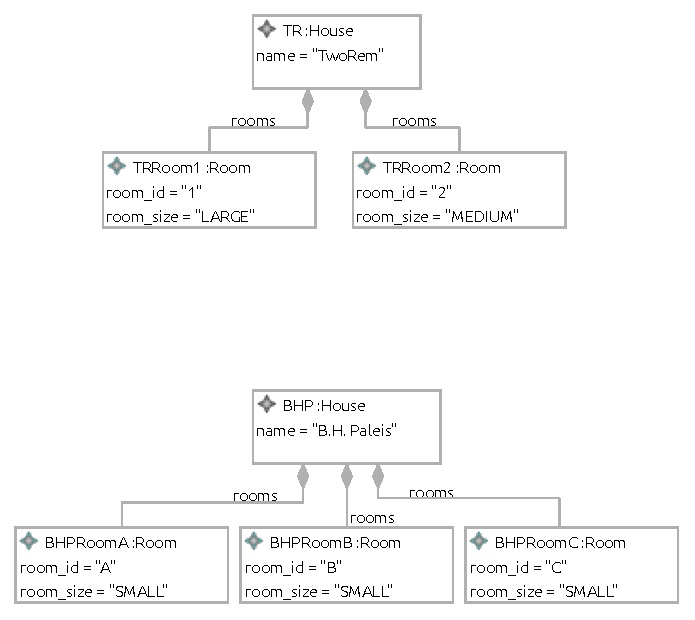
\includegraphics{images/06_application/instance_model/step07.pdf}
        \caption{Instance Model $Im_7$}
        \label{fig:application:building_the_model:room_sizes:ecore:instance_model}
    \end{subfigure}
    \\
    \begin{subfigure}{0.98\textwidth}
        \centering
        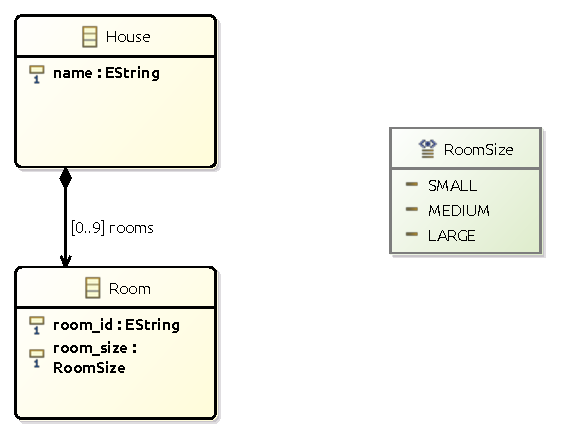
\includegraphics{images/06_application/type_model/step07.pdf}
        \caption{Type Model $Tm_7$}
        \label{fig:application:building_the_model:room_sizes:ecore:type_model}
    \end{subfigure}
    \caption{The Ecore model after step 7}
    \label{fig:application:building_the_model:room_sizes:ecore}
\end{figure}

\begin{figure}[p]
    \centering
    \begin{subfigure}{0.98\textwidth}
        \centering
        % To use this figure in your LaTeX document
% import the package groove/resources/groove2tikz.sty
%
\begin{tikzpicture}[scale=\tikzscale,name prefix=step07-]
\node[type_node] (n0) at (0.740, -0.400) {\ml{\textbf{House}\\name: \textbf{string}}};
\node[type_node] (n1) at (0.730, -1.585) {\ml{\textbf{Room}\\room\_id: \textbf{string}}};
\node[type_node] (n2) at (2.380, -0.560) {\ml{\textbf{RoomSize}\\\textit{LARGE}\\\textit{MEDIUM}\\\textit{SMALL}}};

\path[basic_edge, composite](n0.south -| 0.730, -1.585) -- node[lab] {\ml{rooms}} (n1) ;
\path[basic_edge] (n1)  -- node[lab] {\ml{room\_size}} (n2) ;
\end{tikzpicture}

        \caption{Instance Graph $IG_7$}
        \label{fig:application:building_the_model:room_sizes:groove:instance_graph}
    \end{subfigure}
    \\
    \begin{subfigure}{0.98\textwidth}
        \centering
        % To use this figure in your LaTeX document
% import the package groove/resources/groove2tikz.sty
%
\begin{tikzpicture}[scale=\tikzscale,name prefix=step07-]
\node[type_node] (n0) at (0.740, -0.400) {\ml{\textbf{House}\\name: \textbf{string}}};
\node[type_node] (n1) at (0.730, -1.585) {\ml{\textbf{Room}\\room\_id: \textbf{string}}};
\node[type_node] (n2) at (2.380, -0.560) {\ml{\textbf{RoomSize}\\\textit{LARGE}\\\textit{MEDIUM}\\\textit{SMALL}}};

\path[basic_edge, composite](n0.south -| 0.730, -1.585) -- node[lab] {\ml{rooms}} (n1) ;
\path[basic_edge] (n1)  -- node[lab] {\ml{room\_size}} (n2) ;
\end{tikzpicture}

        \caption{Type Graph $TG_7$}
        \label{fig:application:building_the_model:room_sizes:groove:type_graph}
    \end{subfigure}
    \caption{The GROOVE graphs after step 7}
    \label{fig:application:building_the_model:room_sizes:groove}
\end{figure}

A visual representation of $Tm_7$ and $Im_7$ can be found in \cref{fig:application:building_the_model:room_sizes:ecore}. Similarly, a visual representation of $TG_7$ and $IG_7$ can be found in \cref{fig:application:building_the_model:room_sizes:groove}. Please note that because of the definitions of $f_7(Im_7)$ and $f'_7(IG_7)$, we have that $f_7(Im_7) = IG_7$ and $f'_7(IG_7) = Im_7$. Furthermore, $f_7(Im_7)$ and $f'_7(IG_7)$ are valid mapping functions themselves, such that they can be combined with another mapping function in the next step.

On the instance model level, no surprising elements are introduced. An enumeration field acts like most other attributes within Ecore. However, the visualisation shows how enumeration values are referenced by their instance nodes in the instance graph. The encoding of the field makes use of the presented encoding to emulate enumeration types within GROOVE.

\afterpage{\FloatBarrier}
\subsection{Tenants}
\label{sec:application:building_the_model:tenants}

The eighth step introduces another class type. This time, the $.\type{Tenant}$ type is introduced to enrich the model and graphs even further. \cref{subsec:library_of_transformations:type_level_transformations:regular_classes} is used to introduce the class type, while on the instance level, \cref{subsec:library_of_transformations:instance_level_transformations:plain_objects} is used to introduce the house objects.

The $name$ of the new tenant type is $.\type{Tenant}$. Furthermore, 5 tenant objects are introduced, $objects = \{Tenant1, Tenant2, Tenant3, Tenant4, Tenant5\}$. Furthermore, we assume that the object identifiers are equal to the internal node id, so $fid(Tenant1) = Tenant1$ and $fid(Tenant2) = Tenant2$, etc. The following model is obtained:

\LTXtable{\textwidth}{tex/06_application/02_building_the_model/tables/08_tenants.tex}

\begin{figure}[p]
    \centering
    \begin{subfigure}{0.98\textwidth}
        \centering
        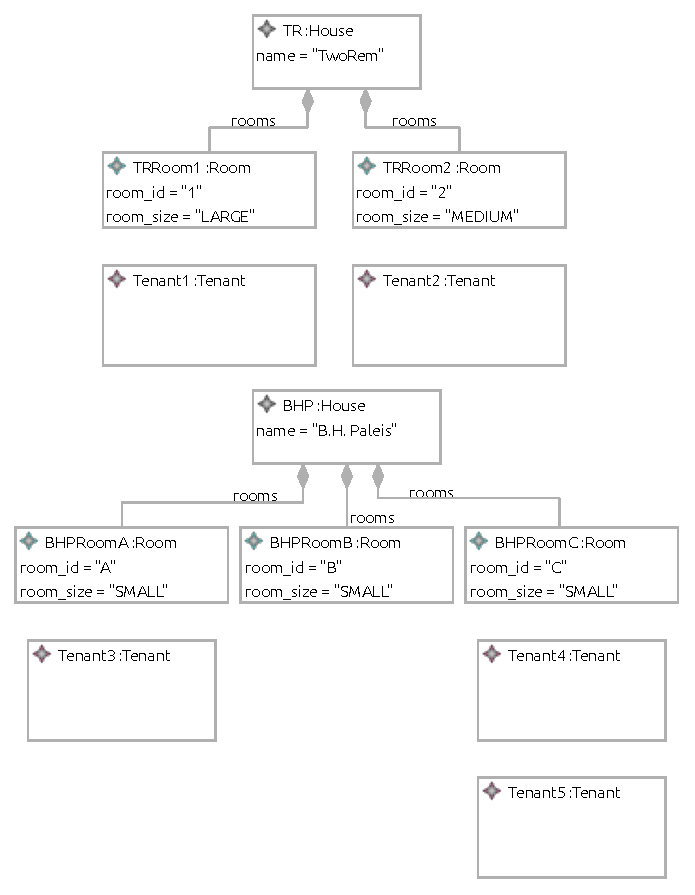
\includegraphics{images/06_application/instance_model/step08.pdf}
        \caption{Instance Model $Im_8$}
        \label{fig:application:building_the_model:tenants:ecore:instance_model}
    \end{subfigure}
    \\
    \begin{subfigure}{0.98\textwidth}
        \centering
        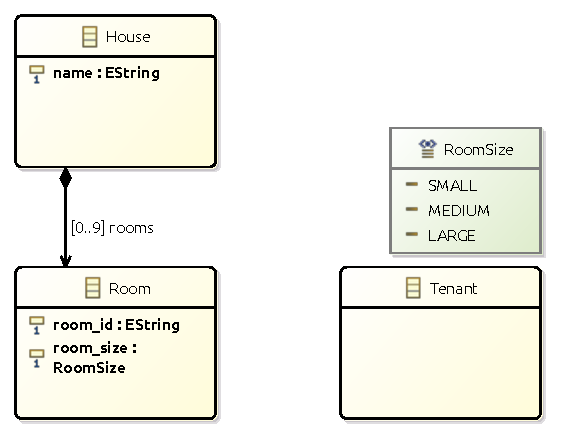
\includegraphics{images/06_application/type_model/step08.pdf}
        \caption{Type Model $Tm_8$}
        \label{fig:application:building_the_model:tenants:ecore:type_model}
    \end{subfigure}
    \caption{The Ecore model after step 8}
    \label{fig:application:building_the_model:tenants:ecore}
\end{figure}

\begin{figure}[p]
    \centering
    \begin{subfigure}{0.98\textwidth}
        \centering
        % To use this figure in your LaTeX document
% import the package groove/resources/groove2tikz.sty
%
\begin{tikzpicture}[scale=\tikzscale,name prefix=step08-]
\node[type_node] (n0) at (0.740, -0.400) {\ml{\textbf{House}\\name: \textbf{string}}};
\node[type_node] (n1) at (0.730, -1.585) {\ml{\textbf{Room}\\room\_id: \textbf{string}}};
\node[type_node] (n2) at (2.380, -0.560) {\ml{\textbf{RoomSize}\\\textit{LARGE}\\\textit{MEDIUM}\\\textit{SMALL}}};
\node[type_node] (n3) at (2.500, -1.590) {\ml{\textbf{Tenant}}};

\path[basic_edge, composite](n0.south -| 0.730, -1.585) -- node[lab] {\ml{rooms}} (n1) ;
\path[basic_edge] (n1)  -- node[lab] {\ml{room\_size}} (n2) ;
\end{tikzpicture}

        \caption{Instance Graph $IG_8$}
        \label{fig:application:building_the_model:tenants:groove:instance_graph}
    \end{subfigure}
    \\
    \begin{subfigure}{0.98\textwidth}
        \centering
        % To use this figure in your LaTeX document
% import the package groove/resources/groove2tikz.sty
%
\begin{tikzpicture}[scale=\tikzscale,name prefix=step08-]
\node[type_node] (n0) at (0.740, -0.400) {\ml{\textbf{House}\\name: \textbf{string}}};
\node[type_node] (n1) at (0.730, -1.585) {\ml{\textbf{Room}\\room\_id: \textbf{string}}};
\node[type_node] (n2) at (2.380, -0.560) {\ml{\textbf{RoomSize}\\\textit{LARGE}\\\textit{MEDIUM}\\\textit{SMALL}}};
\node[type_node] (n3) at (2.500, -1.590) {\ml{\textbf{Tenant}}};

\path[basic_edge, composite](n0.south -| 0.730, -1.585) -- node[lab] {\ml{rooms}} (n1) ;
\path[basic_edge] (n1)  -- node[lab] {\ml{room\_size}} (n2) ;
\end{tikzpicture}

        \caption{Type Graph $TG_8$}
        \label{fig:application:building_the_model:tenants:groove:type_graph}
    \end{subfigure}
    \caption{The GROOVE graphs after step 8}
    \label{fig:application:building_the_model:tenants:groove}
\end{figure}

A visual representation of $Tm_8$ and $Im_8$ can be found in \cref{fig:application:building_the_model:tenants:ecore}. Similarly, a visual representation of $TG_8$ and $IG_8$ can be found in \cref{fig:application:building_the_model:tenants:groove}. Please note that because of the definitions of $f_8(Im_8)$ and $f'_8(IG_8)$, we have that $f_8(Im_8) = IG_8$ and $f'_8(IG_8) = Im_8$. Furthermore, $f_8(Im_8)$ and $f'_8(IG_8)$ are valid mapping functions themselves, such that they can be combined with another mapping function in the next step.

The introduction of the tenant class shows that models can be extended if there is already much information in the model. Introducing types can be done at any moment, so there is no need to introduce all types at the beginning. In that sense, the transformation framework presented by this thesis is not deterministic; there are multiple ways to encode the same model.

\afterpage{\FloatBarrier}
\begin{longtable}{|lX|}
\hline
\multicolumn{2}{|l|}{\textbf{Models after step 9}}\\
\hhline{|==|}
\endhead
$Tm_9 = $ & $\mathrm{combine}(Tm_8, Tm_{DataField}) =$ \newline
$\begin{aligned}
Class =\ & \{.\type{House}, .\type{Room}, .\type{Tenant}\} \\
Enum =\ & \{.\type{RoomSize}\} \\
UserDataType =\ & \{\} \\
Field =\ & \{(.\type{House}, \type{name}), (.\type{House}, \type{rooms}), (.\type{Room}, \type{room\_\!id}), \\& (.\type{Room}, \type{room\_size}), (.\type{Tenant}, \type{name})\} \\
\mathrm{FieldSig} =\ & \big\{
\big((.\type{House}, \type{name}), (\type{string}, 1..1)\big),\\&
\big((.\type{House}, \type{rooms}), ([\type{setof}, !.\type{Room}], 0..9)\big),\\&
\big((.\type{Room}, \type{room\_\!id}), (\type{string}, 1..1)\big),\\&
\big((.\type{Room}, \type{room\_size}), (.\type{RoomSize}, 1..1)\big),\\&
\big((.\type{Tenant}, \type{name}), (\type{string}, 1..1)\big)
\big\} \\
EnumValue =\ & \{(.\type{RoomSize}, \type{SMALL}), (.\type{RoomSize}, \type{MEDIUM}), (.\type{RoomSize}, \type{LARGE})\} \\
Inh =\ & \{\} \\
Prop =\ & \big\{\big(\type{containment}, (.\type{House}, \type{rooms})\big)\big\} \\
Constant =\ & \{\} \\
\mathrm{ConstType} =\ & \{\}
\end{aligned}$
\\
$Im_9 = $ & $\mathrm{combine}(Tm_8, Im_{DataField}) =$ \newline
$\begin{aligned}
Object =\ &\{TR, BHP, TRRoom1, TRRoom2, BHPRoomA, BHPRoomB, \\& BHPRoomC, Tenant1, Tenant2, Tenant3, Tenant4, Tenant5\} \\
\mathrm{ObjectClass}(ob) =\ & \{(TR, .\type{House}), (BHP, .\type{House}),
(TRRoom1, .\type{Room}),\\& (TRRoom2, .\type{Room}), (BHPRoomA, .\type{Room}), (BHPRoomB, .\type{Room}),\\& (BHPRoomC, .\type{Room}, (Tenant1, .\type{Tenant}), (Tenant2, .\type{Tenant}), \\& (Tenant3, .\type{Tenant}), (Tenant4, .\type{Tenant}), (Tenant5, .\type{Tenant})\}\\
\mathrm{ObjectId} =\ & \{(TR, TR), (BHP, BHP), (TRRoom1, TRRoom1),\\& (TRRoom2, TRRoom2), (BHPRoomA, BHPRoomA),\\& (BHPRoomB, BHPRoomB), (BHPRoomC, BHPRoomC), \\&(Tenant1, Tenant1), (Tenant2, Tenant2), (Tenant3, Tenant3),\\& (Tenant4, Tenant4), (Tenant5, Tenant5)\}\\
\mathrm{FieldValue} =\ & \Big\{
\Big(\big(TR, (.\type{House}, \type{name})\big), \big[\type{string}, \text{``TwoRem''}\big]\Big),\\&
\Big(\big(BHP, (.\type{House}, \type{name})\big), \big[\type{string}, \text{``B.H. Paleis''}\big]\Big),\\&
\Big(\big(TR, (.\type{House}, \type{rooms})\big), \big[\type{setof}, \big\langle [\type{obj}, TRRoom1], \\&\qquad [\type{obj}, TRRoom2] \big\rangle \big]\Big),\\&
\Big(\big(BHP, (.\type{House}, \type{rooms})\big) \big[\type{setof}, \big\langle [\type{obj},  BHPRoomA], \\&\qquad [\type{obj}, BHPRoomB], (\type{obj}, BHPRoomC) \big\rangle \big]\Big),\\&
\Big(\big(TRRoom1, (.\type{Room}, \type{room\_\!id})\big), \big[\type{string}, \text{``1''}\big]\Big),\\&
\Big(\big(TRRoom2, (.\type{Room}, \type{room\_\!id})\big), \big[\type{string}, \text{``2''}\big]\Big),\\&
\Big(\big(BHPRoomA, (.\type{Room}, \type{room\_\!id})\big), \big[\type{string}, \text{``A''}\big]\Big),\\&
\Big(\big(BHPRoomB, (.\type{Room}, \type{room\_\!id})\big), \big[\type{string}, \text{``B''}\big]\Big),\\&
\Big(\big(BHPRoomC, (.\type{Room}, \type{room\_\!id})\big), \big[\type{string}, \text{``C''}\big]\Big),\\&
\Big(\big(TRRoom1, (.\type{Room}, \type{room\_size})\big), \big[\type{enum}, (.\type{RoomSize}, \type{LARGE}) \big]\Big),\\&
\Big(\big(TRRoom2, (.\type{Room}, \type{room\_size})\big), \big[\type{enum}, (.\type{RoomSize}, \type{MEDIUM}) \big]\Big),\\&
\Big(\big(BHPRoomA, (.\type{Room}, \type{room\_size})\big), \big[\type{enum}, (.\type{RoomSize}, \type{SMALL}) \big]\Big),\\&
\Big(\big(BHPRoomB, (.\type{Room}, \type{room\_size})\big), \big[\type{enum}, (.\type{RoomSize}, \type{SMALL}) \big]\Big),\\&
\Big(\big(BHPRoomC, (.\type{Room}, \type{room\_size})\big), \big[\type{enum}, (.\type{RoomSize}, \type{SMALL}) \big]\Big),\\&
\Big(\big(Tenant1, (.\type{Tenant}, \type{name})\big), \big[\type{string}, \text{``B.R. Mankjon''}\big]\Big),\\&
\Big(\big(Tenant2, (.\type{Tenant}, \type{name})\big), \big[\type{string}, \text{``P.J.R. Nam''}\big]\Big),\\&
\Big(\big(Tenant3, (.\type{Tenant}, \type{name})\big), \big[\type{string}, \text{``L. Horn''}\big]\Big),\\&
\Big(\big(Tenant4, (.\type{Tenant}, \type{name})\big), \big[\type{string}, \text{``A.C.C. Turg''}\big]\Big),\\&
\Big(\big(Tenant5, (.\type{Tenant}, \type{name})\big), \big[\type{string}, \text{``M. Silon''}\big]\Big)
\Big\} \\
\mathrm{DefaultValue} =\ & \{\}
\end{aligned}$
\\
\hline
$TG_9 = $ & $\mathrm{combine}(TG_8, TG_{DataField}) =$ \newline
$\begin{aligned}
NT =\ & \{\langle \type{House} \rangle, \langle \type{Room} \rangle, \langle \type{Tenant} \rangle, \langle \type{RoomSize} \rangle, \type{string}\} \\
ET =\ & \big\{
\big(\langle \type{House} \rangle, \langle \type{name} \rangle, \type{string} \big),
\big(\langle \type{House} \rangle, \langle \type{rooms} \rangle, \langle \type{Room} \rangle \big),\\&
\big(\langle \type{Room} \rangle, \langle \type{room\_\!id} \rangle, \type{string} \big),
\big(\langle \type{Room} \rangle, \langle \type{room\_size} \rangle, \langle \type{RoomSize} \rangle \big),\\&
\big(\langle \type{Tenant} \rangle, \langle \type{name} \rangle, \type{string} \big),
\big(\langle \type{RoomSize} \rangle, \langle \type{SMALL} \rangle, \langle \type{RoomSize} \rangle \big),\\&
\big(\langle \type{RoomSize} \rangle, \langle \type{MEDIUM} \rangle, \langle \type{RoomSize} \rangle \big),
\big(\langle \type{RoomSize} \rangle, \langle \type{LARGE} \rangle, \langle \type{RoomSize} \rangle \big)
\big\} \\
\!\!\sqsubseteq\ =\ & \big\{
\big(\langle \type{House} \rangle, \langle \type{House} \rangle \big),
\big(\langle \type{Room} \rangle, \langle \type{Room} \rangle \big),
\big(\langle \type{Tenant} \rangle, \langle \type{Tenant} \rangle \big),\\&
\big(\langle \type{RoomSize} \rangle, \langle \type{RoomSize} \rangle \big),
\big(\type{string}, \type{string} \big)
\big\} \\
abs =\ & \{\} \\
\mathrm{mult} =\ & \Big\{
\Big(\big(\langle \type{House} \rangle, \langle \type{name} \rangle, \type{string} \big), \big(0..\mstar, 1..1\big) \Big),\\&
\Big(\big(\langle \type{House} \rangle, \langle \type{rooms} \rangle, \langle \type{Room} \rangle \big), \big(0..1, 0..9\big) \Big),\\&
\Big(\big(\langle \type{Room} \rangle, \langle \type{room\_\!id} \rangle, \type{string} \big), \big(0..\mstar, 1..1\big) \Big),\\&
\Big(\big(\langle \type{Room} \rangle, \langle \type{room\_size} \rangle, \langle \type{RoomSize} \rangle \big), \big(0..\mstar, 1..1\big) \Big),\\&
\Big(\big(\langle \type{Tenant} \rangle, \langle \type{name} \rangle, \type{string} \big), \big(0..\mstar, 1..1\big) \Big),\\&
\Big(\big(\langle \type{RoomSize} \rangle, \langle \type{SMALL} \rangle, \langle \type{RoomSize} \rangle \big), \big(0..1, 0..1\big) \Big),\\&
\Big(\big(\langle \type{RoomSize} \rangle, \langle \type{MEDIUM} \rangle, \langle \type{RoomSize} \rangle \big), \big(0..1, 0..1\big) \Big),\\&
\Big(\big(\langle \type{RoomSize} \rangle, \langle \type{LARGE} \rangle, \langle \type{RoomSize} \rangle \big), \big(0..1, 0..1\big) \Big)
\Big\} \\
contains =\ & \big\{\big(\langle \type{House} \rangle, \langle \type{rooms} \rangle, \langle \type{Room} \rangle \big)\big\}
\end{aligned}$
\\
$IG_9 = $ & $\mathrm{combine}(TG_8, IG_{DataField}) =$ \newline
$\begin{aligned}
N =\ & \{TR, BHP, TRRoom1, TRRoom2, BHPRoomA, BHPRoomB, BHPRoomC, \\& 
Tenant1, Tenant2, Tenant3, Tenant4, Tenant5, SmallSize, MediumSize,\\& LargeSize,
\text{``TwoRem''}, \text{``B.H. Paleis''}, \text{``1''},  \text{``2''}, \text{``A''}, \text{``B''}, \text{``C''}, \text{``B.R. Mankjon''}, \\& \text{``P.J.R. Nam''}, \text{``L. Horn''}, \text{``A.C.C. Turg''}, \text{``M. Silon''}\} \\
E =\ & \Big\{
\Big(TR, \big(\langle \type{House} \rangle, \langle \type{name} \rangle, \type{string} \big), \text{``TwoRem''} \Big),\\&
\Big(BHP, \big(\langle \type{House} \rangle, \langle \type{name} \rangle, \type{string} \big), \text{``B.H. Paleis''} \Big),\\&
\Big(TR, \big(\langle \type{House} \rangle, \langle \type{rooms} \rangle, \langle \type{Room} \rangle \big), TRRoom1 \Big),\\&
\Big(TR, \big(\langle \type{House} \rangle, \langle \type{rooms} \rangle, \langle \type{Room} \rangle \big), TRRoom2 \Big),\\&
\Big(BHP, \big(\langle \type{House} \rangle, \langle \type{rooms} \rangle, \langle \type{Room} \rangle \big), BHPRoomA \Big),\\&
\Big(BHP, \big(\langle \type{House} \rangle, \langle \type{rooms} \rangle, \langle \type{Room} \rangle \big), BHPRoomB \Big),\\&
\Big(BHP, \big(\langle \type{House} \rangle, \langle \type{rooms} \rangle, \langle \type{Room} \rangle \big), BHPRoomC \Big),\\&
\Big(TRRoom1, \big(\langle \type{Room} \rangle, \langle \type{room\_\!id} \rangle, \type{string} \big), \text{``1''} \Big),\\&
\Big(TRRoom2, \big(\langle \type{Room} \rangle, \langle \type{room\_\!id} \rangle, \type{string} \big), \text{``2''} \Big),\\&
\Big(BHPRoomA, \big(\langle \type{Room} \rangle, \langle \type{room\_\!id} \rangle, \type{string} \big), \text{``A''} \Big),\\&
\Big(BHPRoomB, \big(\langle \type{Room} \rangle, \langle \type{room\_\!id} \rangle, \type{string} \big), \text{``B''} \Big),\\&
\Big(BHPRoomC, \big(\langle \type{Room} \rangle, \langle \type{room\_\!id} \rangle, \type{string} \big), \text{``C''} \Big),\\&
\Big(TRRoom1, \big(\langle \type{Room} \rangle, \langle \type{room\_size} \rangle, \langle \type{RoomSize} \rangle \big), LargeSize \Big),\\&
\Big(TRRoom2, \big(\langle \type{Room} \rangle, \langle \type{room\_size} \rangle, \langle \type{RoomSize} \rangle \big), MediumSize \Big),\\&
\Big(BHPRoomA, \big(\langle \type{Room} \rangle, \langle \type{room\_size} \rangle, \langle \type{RoomSize} \rangle \big), SmallSize \Big),\\&
\Big(BHPRoomB, \big(\langle \type{Room} \rangle, \langle \type{room\_size} \rangle, \langle \type{RoomSize} \rangle \big), SmallSize \Big),\\&
\Big(BHPRoomC, \big(\langle \type{Room} \rangle, \langle \type{room\_size} \rangle, \langle \type{RoomSize} \rangle \big), SmallSize \Big),\\&
\Big(Tenant1, \big(\langle \type{Tenant} \rangle, \langle \type{name} \rangle, \type{string} \big), \text{``B.R. Mankjon''} \Big),\\&
\Big(Tenant2, \big(\langle \type{Tenant} \rangle, \langle \type{name} \rangle, \type{string} \big), \text{``P.J.R. Nam''} \Big),\\&
\Big(Tenant3, \big(\langle \type{Tenant} \rangle, \langle \type{name} \rangle, \type{string} \big), \text{``L. Horn''} \Big),\\&
\Big(Tenant4, \big(\langle \type{Tenant} \rangle, \langle \type{name} \rangle, \type{string} \big), \text{``A.C.C. Turg''} \Big),\\&
\Big(Tenant5, \big(\langle \type{Tenant} \rangle, \langle \type{name} \rangle, \type{string} \big), \text{``M. Silon''} \Big),\\&
\Big(SmallSize, \big(\langle \type{RoomSize} \rangle, \langle \type{SMALL} \rangle, \langle \type{RoomSize} \rangle \big), SmallSize \Big),\\&
\Big(MediumSize, \big(\langle \type{RoomSize} \rangle, \langle \type{MEDIUM} \rangle, \langle \type{RoomSize} \rangle \big), MediumSize \Big),\\&
\Big(LargeSize, \big(\langle \type{RoomSize} \rangle, \langle \type{LARGE} \rangle, \langle \type{RoomSize} \rangle \big), LargeSize \Big)
\Big\}
\end{aligned}$
\\&
$\begin{aligned}
\mathrm{ident} =\ & \{(TR, TR), (BHP, BHP), (TRRoom1, TRRoom1), (TRRoom2, TRRoom2),\\& (BHPRoomA, BHPRoomA), (BHPRoomB, BHPRoomB),\\& (BHPRoomC, BHPRoomC), (Tenant1, Tenant1), (Tenant2, Tenant2),\\& (Tenant3, Tenant3), (Tenant4, Tenant4), (Tenant5, Tenant5),\\& (SmallSize, SmallSize), (MediumSize, MediumSize),\\& (LargeSize, LargeSize)\}\\
\mathrm{type}_n =\ & \{
(TR, \langle \type{House} \rangle), 
(BHP, \langle \type{House} \rangle),
(TRRoom1, \langle \type{Room} \rangle),
(TRRoom2, \langle \type{Room} \rangle),\\&
(BHPRoomA, \langle \type{Room} \rangle),
(BHPRoomB, \langle \type{Room} \rangle),
(BHPRoomC, \langle \type{Room} \rangle),\\&
(Tenant1, \langle \type{Tenant} \rangle),
(Tenant2, \langle \type{Tenant} \rangle),
(Tenant3, \langle \type{Tenant} \rangle),\\&
(Tenant4, \langle \type{Tenant} \rangle),
(Tenant5, \langle \type{Tenant} \rangle),
(SmallSize, \langle \type{RoomSize} \rangle),\\&
(MediumSize, \langle \type{RoomSize} \rangle),
(LargeSize, \langle \type{RoomSize} \rangle),
(\text{``TwoRem''}, \type{string}),\\&
(\text{``B.H. Paleis''}, \type{string}),
(\text{``1''}, \type{string}),
(\text{``2''}, \type{string}),
(\text{``A''}, \type{string}),
(\text{``B''}, \type{string}),\\&
(\text{``C''}, \type{string}),
(\text{``B.R. Mankjon''}, \type{string}),
(\text{``P.J.R. Nam''}, \type{string}),\\&
(\text{``A.C.C. Turg''}, \type{string}),
(\text{``L. Horn''}, \type{string}),
(\text{``M. Silon''}, \type{string})
\}
\end{aligned}$
\\
\hline
$f_9(Im_9) = $ & $f_8(Im_8) \sqcup f_{DataField}(Im_{DataField})$  (\cref{defin:transformation_framework:instance_models_and_instance_graphs:combining_transformation_functions:combination_transformation_function_instance_model_instance_graph})\\
$f'_9(IG_9) = $ & $f'_8(IG_8) \sqcup f'_{DataField}(IG_{DataField})$  (\cref{defin:transformation_framework:instance_models_and_instance_graphs:combining_transformation_functions:combination_transformation_function_instance_graph_instance_model})\\
\hline
\end{longtable}
\begin{longtable}{|lX|}
\hline
\multicolumn{2}{|l|}{\textbf{Models after step 10}}\\
\hhline{|==|}
\endhead
$Tm_{10} = $ & $\mathrm{combine}(Tm_9, Tm_{DataField}) =$ \newline
$\begin{aligned}
Class =\ & \{.\type{House}, .\type{Room}, .\type{Tenant}\} \\
Enum =\ & \{.\type{RoomSize}\} \\
UserDataType =\ & \{\} \\
Field =\ & \{(.\type{House}, \type{name}), (.\type{House}, \type{rooms}), (.\type{Room}, \type{room\_\!id}), \\& (.\type{Room}, \type{room\_size}), (.\type{Tenant}, \type{name}), (.\type{Tenant}, \type{age})\} \\
\mathrm{FieldSig} =\ & \big\{
\big((.\type{House}, \type{name}), (\type{string}, 1..1)\big),\\&
\big((.\type{House}, \type{rooms}), ([\type{setof}, !.\type{Room}], 0..9)\big),\\&
\big((.\type{Room}, \type{room\_\!id}), (\type{string}, 1..1)\big),\\&
\big((.\type{Room}, \type{room\_size}), (.\type{RoomSize}, 1..1)\big),\\&
\big((.\type{Tenant}, \type{name}), (\type{string}, 1..1)\big),\\&
\big((.\type{Tenant}, \type{age}), (\type{int}, 1..1)\big)
\big\} \\
EnumValue =\ & \{(.\type{RoomSize}, \type{SMALL}), (.\type{RoomSize}, \type{MEDIUM}), (.\type{RoomSize}, \type{LARGE})\} \\
Inh =\ & \{\} \\
Prop =\ & \big\{\big(\type{containment}, (.\type{House}, \type{rooms})\big)\big\} \\
Constant =\ & \{\} \\
\mathrm{ConstType} =\ & \{\}
\end{aligned}$
\\
$Im_{10} = $ & $\mathrm{combine}(Tm_9, Im_{DataField}) =$ \newline
$\begin{aligned}
Object =\ &\{TR, BHP, TRRoom1, TRRoom2, BHPRoomA, BHPRoomB, \\& BHPRoomC, Tenant1, Tenant2, Tenant3, Tenant4, Tenant5\} \\
\mathrm{ObjectClass}(ob) =\ & \{(TR, .\type{House}), (BHP, .\type{House}),
(TRRoom1, .\type{Room}),\\& (TRRoom2, .\type{Room}), (BHPRoomA, .\type{Room}), (BHPRoomB, .\type{Room}),\\& (BHPRoomC, .\type{Room}, (Tenant1, .\type{Tenant}), (Tenant2, .\type{Tenant}), \\& (Tenant3, .\type{Tenant}), (Tenant4, .\type{Tenant}), (Tenant5, .\type{Tenant})\}\\
\mathrm{ObjectId} =\ & \{(TR, TR), (BHP, BHP), (TRRoom1, TRRoom1),\\& (TRRoom2, TRRoom2), (BHPRoomA, BHPRoomA),\\& (BHPRoomB, BHPRoomB), (BHPRoomC, BHPRoomC), \\&(Tenant1, Tenant1), (Tenant2, Tenant2), (Tenant3, Tenant3),\\& (Tenant4, Tenant4), (Tenant5, Tenant5)\}\\
\mathrm{FieldValue} =\ & \Big\{
\Big(\big(TR, (.\type{House}, \type{name})\big), \big[\type{string}, \text{``TwoRem''}\big]\Big),\\&
\Big(\big(BHP, (.\type{House}, \type{name})\big), \big[\type{string}, \text{``B.H. Paleis''}\big]\Big),\\&
\Big(\big(TR, (.\type{House}, \type{rooms})\big), \big[\type{setof}, \big\langle [\type{obj}, TRRoom1], \\&\qquad [\type{obj}, TRRoom2] \big\rangle \big]\Big),\\&
\Big(\big(BHP, (.\type{House}, \type{rooms})\big) \big[\type{setof}, \big\langle [\type{obj},  BHPRoomA], \\&\qquad [\type{obj}, BHPRoomB], (\type{obj}, BHPRoomC) \big\rangle \big]\Big),\\&
\Big(\big(TRRoom1, (.\type{Room}, \type{room\_\!id})\big), \big[\type{string}, \text{``1''}\big]\Big),\\&
\Big(\big(TRRoom2, (.\type{Room}, \type{room\_\!id})\big), \big[\type{string}, \text{``2''}\big]\Big),\\&
\Big(\big(BHPRoomA, (.\type{Room}, \type{room\_\!id})\big), \big[\type{string}, \text{``A''}\big]\Big),\\&
\Big(\big(BHPRoomB, (.\type{Room}, \type{room\_\!id})\big), \big[\type{string}, \text{``B''}\big]\Big),\\&
\Big(\big(BHPRoomC, (.\type{Room}, \type{room\_\!id})\big), \big[\type{string}, \text{``C''}\big]\Big),\\&
\Big(\big(TRRoom1, (.\type{Room}, \type{room\_size})\big), \big[\type{enum}, (.\type{RoomSize}, \type{LARGE}) \big]\Big),\\&
\Big(\big(TRRoom2, (.\type{Room}, \type{room\_size})\big), \big[\type{enum}, (.\type{RoomSize}, \type{MEDIUM}) \big]\Big),\\&
\Big(\big(BHPRoomA, (.\type{Room}, \type{room\!\_\!size})\big), \big[\type{enum}, (.\type{RoomSize}, \type{SMALL}) \big]\Big),\\&
\Big(\big(BHPRoomB, (.\type{Room}, \type{room\!\_\!size})\big), \big[\type{enum}, (.\type{RoomSize}, \type{SMALL}) \big]\Big),\\&
\Big(\big(BHPRoomC, (.\type{Room}, \type{room\!\_\!size})\big), \big[\type{enum}, (.\type{RoomSize}, \type{SMALL}) \big]\Big),\\&
\Big(\big(Tenant1, (.\type{Tenant}, \type{name})\big), \big[\type{string}, \text{``B.R. Mankjon''}\big]\Big),\\&
\Big(\big(Tenant2, (.\type{Tenant}, \type{name})\big), \big[\type{string}, \text{``P.J.R. Nam''}\big]\Big),\\&
\Big(\big(Tenant3, (.\type{Tenant}, \type{name})\big), \big[\type{string}, \text{``L. Horn''}\big]\Big),\\&
\Big(\big(Tenant4, (.\type{Tenant}, \type{name})\big), \big[\type{string}, \text{``A.C.C. Turg''}\big]\Big),\\&
\Big(\big(Tenant5, (.\type{Tenant}, \type{name})\big), \big[\type{string}, \text{``M. Silon''}\big]\Big),\\&
\Big(\big(Tenant1, (.\type{Tenant}, \type{age})\big), \big[\type{int}, 23\big]\Big),\\&
\Big(\big(Tenant2, (.\type{Tenant}, \type{age})\big), \big[\type{int}, 24\big]\Big),\\&
\Big(\big(Tenant3, (.\type{Tenant}, \type{age})\big), \big[\type{int}, 18\big]\Big),\\&
\Big(\big(Tenant4, (.\type{Tenant}, \type{age})\big), \big[\type{int}, 24\big]\Big),\\&
\Big(\big(Tenant5, (.\type{Tenant}, \type{age})\big), \big[\type{int}, 19\big]\Big)
\Big\} \\
\mathrm{DefaultValue} =\ & \{\}
\end{aligned}$
\\
\hline
$TG_{10} = $ & $\mathrm{combine}(TG_9, TG_{DataField}) =$ \newline
$\begin{aligned}
NT =\ & \{\langle \type{House} \rangle, \langle \type{Room} \rangle, \langle \type{Tenant} \rangle, \langle \type{RoomSize} \rangle, \type{string}, \type{int}\} \\
ET =\ & \big\{
\big(\langle \type{House} \rangle, \langle \type{name} \rangle, \type{string} \big),
\big(\langle \type{House} \rangle, \langle \type{rooms} \rangle, \langle \type{Room} \rangle \big),\\&
\big(\langle \type{Room} \rangle, \langle \type{room\_\!id} \rangle, \type{string} \big),
\big(\langle \type{Room} \rangle, \langle \type{room\_size} \rangle, \langle \type{RoomSize} \rangle \big),\\&
\big(\langle \type{Tenant} \rangle, \langle \type{name} \rangle, \type{string} \big),
\big(\langle \type{Tenant} \rangle, \langle \type{age} \rangle, \type{int} \big),\\&
\big(\langle \type{RoomSize} \rangle, \langle \type{SMALL} \rangle, \langle \type{RoomSize} \rangle \big),
\big(\langle \type{RoomSize} \rangle, \langle \type{MEDIUM} \rangle, \langle \type{RoomSize} \rangle \big),\\&
\big(\langle \type{RoomSize} \rangle, \langle \type{LARGE} \rangle, \langle \type{RoomSize} \rangle \big)
\big\} \\
\!\!\sqsubseteq\ =\ & \big\{
\big(\langle \type{House} \rangle, \langle \type{House} \rangle \big),
\big(\langle \type{Room} \rangle, \langle \type{Room} \rangle \big),
\big(\langle \type{Tenant} \rangle, \langle \type{Tenant} \rangle \big),\\&
\big(\langle \type{RoomSize} \rangle, \langle \type{RoomSize} \rangle \big),
\big(\type{string}, \type{string} \big),
\big(\type{int}, \type{int} \big)
\big\} \\
abs =\ & \{\} \\
\mathrm{mult} =\ & \Big\{
\Big(\big(\langle \type{House} \rangle, \langle \type{name} \rangle, \type{string} \big), \big(0..\mstar, 1..1\big) \Big),\\&
\Big(\big(\langle \type{House} \rangle, \langle \type{rooms} \rangle, \langle \type{Room} \rangle \big), \big(0..1, 0..9\big) \Big),\\&
\Big(\big(\langle \type{Room} \rangle, \langle \type{room\_\!id} \rangle, \type{string} \big), \big(0..\mstar, 1..1\big) \Big),\\&
\Big(\big(\langle \type{Room} \rangle, \langle \type{room\_size} \rangle, \langle \type{RoomSize} \rangle \big), \big(0..\mstar, 1..1\big) \Big),\\&
\Big(\big(\langle \type{Tenant} \rangle, \langle \type{name} \rangle, \type{string} \big), \big(0..\mstar, 1..1\big) \Big),\\&
\Big(\big(\langle \type{Tenant} \rangle, \langle \type{age} \rangle, \type{int} \big), \big(0..\mstar, 0..1\big) \Big),\\&
\Big(\big(\langle \type{RoomSize} \rangle, \langle \type{SMALL} \rangle, \langle \type{RoomSize} \rangle \big), \big(0..1, 0..1\big) \Big),\\&
\Big(\big(\langle \type{RoomSize} \rangle, \langle \type{MEDIUM} \rangle, \langle \type{RoomSize} \rangle \big), \big(0..1, 0..1\big) \Big),\\&
\Big(\big(\langle \type{RoomSize} \rangle, \langle \type{LARGE} \rangle, \langle \type{RoomSize} \rangle \big), \big(0..1, 0..1\big) \Big)
\Big\} \\
contains =\ & \big\{\big(\langle \type{House} \rangle, \langle \type{rooms} \rangle, \langle \type{Room} \rangle \big)\big\}
\end{aligned}$
\\
$IG_{10} = $ & $\mathrm{combine}(TG_9, IG_{DataField}) =$ \newline
$\begin{aligned}
N =\ & \{TR, BHP, TRRoom1, TRRoom2, BHPRoomA, BHPRoomB, BHPRoomC, \\& 
Tenant1, Tenant2, Tenant3, Tenant4, Tenant5, SmallSize, MediumSize,\\& LargeSize,
\text{``TwoRem''}, \text{``B.H. Paleis''}, \text{``1''},  \text{``2''}, \text{``A''}, \text{``B''}, \text{``C''}, \text{``B.R. Mankjon''}, \\& \text{``P.J.R. Nam''}, \text{``L. Horn''}, \text{``A.C.C. Turg''}, \text{``M. Silon''}, 23, 24, 18, 19\} \\
E =\ & \Big\{
\Big(TR, \big(\langle \type{House} \rangle, \langle \type{name} \rangle, \type{string} \big), \text{``TwoRem''} \Big),\\&
\Big(BHP, \big(\langle \type{House} \rangle, \langle \type{name} \rangle, \type{string} \big), \text{``B.H. Paleis''} \Big),\\&
\Big(TR, \big(\langle \type{House} \rangle, \langle \type{rooms} \rangle, \langle \type{Room} \rangle \big), TRRoom1 \Big),\\&
\Big(TR, \big(\langle \type{House} \rangle, \langle \type{rooms} \rangle, \langle \type{Room} \rangle \big), TRRoom2 \Big),\\&
\Big(BHP, \big(\langle \type{House} \rangle, \langle \type{rooms} \rangle, \langle \type{Room} \rangle \big), BHPRoomA \Big),\\&
\Big(BHP, \big(\langle \type{House} \rangle, \langle \type{rooms} \rangle, \langle \type{Room} \rangle \big), BHPRoomB \Big),\\&
\Big(BHP, \big(\langle \type{House} \rangle, \langle \type{rooms} \rangle, \langle \type{Room} \rangle \big), BHPRoomC \Big),\\&
\Big(TRRoom1, \big(\langle \type{Room} \rangle, \langle \type{room\_\!id} \rangle, \type{string} \big), \text{``1''} \Big),\\&
\Big(TRRoom2, \big(\langle \type{Room} \rangle, \langle \type{room\_\!id} \rangle, \type{string} \big), \text{``2''} \Big),\\&
\Big(BHPRoomA, \big(\langle \type{Room} \rangle, \langle \type{room\_\!id} \rangle, \type{string} \big), \text{``A''} \Big),\\&
\Big(BHPRoomB, \big(\langle \type{Room} \rangle, \langle \type{room\_\!id} \rangle, \type{string} \big), \text{``B''} \Big),\\&
\Big(BHPRoomC, \big(\langle \type{Room} \rangle, \langle \type{room\_\!id} \rangle, \type{string} \big), \text{``C''} \Big),\\&
\Big(TRRoom1, \big(\langle \type{Room} \rangle, \langle \type{room\_size} \rangle, \langle \type{RoomSize} \rangle \big), LargeSize \Big),\\&
\Big(TRRoom2, \big(\langle \type{Room} \rangle, \langle \type{room\_size} \rangle, \langle \type{RoomSize} \rangle \big), MediumSize \Big),\\&
\Big(BHPRoomA, \big(\langle \type{Room} \rangle, \langle \type{room\_size} \rangle, \langle \type{RoomSize} \rangle \big), SmallSize \Big),\\&
\Big(BHPRoomB, \big(\langle \type{Room} \rangle, \langle \type{room\_size} \rangle, \langle \type{RoomSize} \rangle \big), SmallSize \Big),\\&
\Big(BHPRoomC, \big(\langle \type{Room} \rangle, \langle \type{room\_size} \rangle, \langle \type{RoomSize} \rangle \big), SmallSize \Big),\\&
\Big(Tenant1, \big(\langle \type{Tenant} \rangle, \langle \type{name} \rangle, \type{string} \big), \text{``B.R. Mankjon''} \Big),\\&
\Big(Tenant2, \big(\langle \type{Tenant} \rangle, \langle \type{name} \rangle, \type{string} \big), \text{``P.J.R. Nam''} \Big),\\&
\Big(Tenant3, \big(\langle \type{Tenant} \rangle, \langle \type{name} \rangle, \type{string} \big), \text{``L. Horn''} \Big),\\&
\Big(Tenant4, \big(\langle \type{Tenant} \rangle, \langle \type{name} \rangle, \type{string} \big), \text{``A.C.C. Turg''} \Big),\\&
\Big(Tenant5, \big(\langle \type{Tenant} \rangle, \langle \type{name} \rangle, \type{string} \big), \text{``M. Silon''} \Big),\\&
\Big(Tenant1, \big(\langle \type{Tenant} \rangle, \langle \type{age} \rangle, \type{int} \big), 23 \Big),
\Big(Tenant2, \big(\langle \type{Tenant} \rangle, \langle \type{age} \rangle, \type{int} \big), 24 \Big),\\&
\Big(Tenant3, \big(\langle \type{Tenant} \rangle, \langle \type{age} \rangle, \type{int} \big), 18 \Big),
\Big(Tenant4, \big(\langle \type{Tenant} \rangle, \langle \type{age} \rangle, \type{int} \big), 24 \Big),\\&
\Big(Tenant5, \big(\langle \type{Tenant} \rangle, \langle \type{age} \rangle, \type{int} \big), 19 \Big),\\&
\Big(SmallSize, \big(\langle \type{RoomSize} \rangle, \langle \type{SMALL} \rangle, \langle \type{RoomSize} \rangle \big), SmallSize \Big),\\&
\Big(MediumSize, \big(\langle \type{RoomSize} \rangle, \langle \type{MEDIUM} \rangle, \langle \type{RoomSize} \rangle \big), MediumSize \Big),\\&
\Big(LargeSize, \big(\langle \type{RoomSize} \rangle, \langle \type{LARGE} \rangle, \langle \type{RoomSize} \rangle \big), LargeSize \Big)
\Big\}
\end{aligned}$
\\&
$\begin{aligned}
\mathrm{ident} =\ & \{(TR, TR), (BHP, BHP), (TRRoom1, TRRoom1), (TRRoom2, TRRoom2),\\& (BHPRoomA, BHPRoomA), (BHPRoomB, BHPRoomB),\\& (BHPRoomC, BHPRoomC), (Tenant1, Tenant1), (Tenant2, Tenant2),\\& (Tenant3, Tenant3), (Tenant4, Tenant4), (Tenant5, Tenant5),\\& (SmallSize, SmallSize), (MediumSize, MediumSize),\\& (LargeSize, LargeSize)\}\\
\mathrm{type}_n =\ & \{
(TR, \langle \type{House} \rangle), 
(BHP, \langle \type{House} \rangle),
(TRRoom1, \langle \type{Room} \rangle),
(TRRoom2, \langle \type{Room} \rangle),\\&
(BHPRoomA, \langle \type{Room} \rangle),
(BHPRoomB, \langle \type{Room} \rangle),
(BHPRoomC, \langle \type{Room} \rangle),\\&
(Tenant1, \langle \type{Tenant} \rangle),
(Tenant2, \langle \type{Tenant} \rangle),
(Tenant3, \langle \type{Tenant} \rangle),\\&
(Tenant4, \langle \type{Tenant} \rangle),
(Tenant5, \langle \type{Tenant} \rangle),
(SmallSize, \langle \type{RoomSize} \rangle),\\&
(MediumSize, \langle \type{RoomSize} \rangle),
(LargeSize, \langle \type{RoomSize} \rangle),
(\text{``TwoRem''}, \type{string}),\\&
(\text{``B.H. Paleis''}, \type{string}),
(\text{``1''}, \type{string}),
(\text{``2''}, \type{string}),
(\text{``A''}, \type{string}),
(\text{``B''}, \type{string}),\\&
(\text{``C''}, \type{string}),
(\text{``B.R. Mankjon''}, \type{string}),
(\text{``P.J.R. Nam''}, \type{string}),\\&
(\text{``A.C.C. Turg''}, \type{string}),
(\text{``L. Horn''}, \type{string}),
(\text{``M. Silon''}, \type{string}),
(23, \type{int}),\\&
(24, \type{int}),
(18, \type{int}),
(19, \type{int})
\}
\end{aligned}$
\\
\hline
$f_{10}(Im_{10}) = $ & $f_9(Im_9) \sqcup f_{DataField}(Im_{DataField})$  (\cref{defin:transformation_framework:instance_models_and_instance_graphs:combining_transformation_functions:combination_transformation_function_instance_model_instance_graph})\\
$f'_{10}(IG_{10}) = $ & $f'_9(IG_9) \sqcup f'_{DataField}(IG_{DataField})$  (\cref{defin:transformation_framework:instance_models_and_instance_graphs:combining_transformation_functions:combination_transformation_function_instance_graph_instance_model})\\
\hline
\end{longtable}
\begin{longtable}{|lX|}
\hline
\multicolumn{2}{|l|}{\textbf{Models after step 11}}\\
\hhline{|==|}
\endhead
$Tm_{11} = $ & $\mathrm{combine}(Tm_{10}, Tm_{Enum}) =$ \newline
$\begin{aligned}
Class =\ & \{.\type{House}, .\type{Room}, .\type{Tenant}\} \\
Enum =\ & \{.\type{RoomSize}, .\type{TenantType}\} \\
UserDataType =\ & \{\} \\
Field =\ & \{(.\type{House}, \type{name}), (.\type{House}, \type{rooms}), (.\type{Room}, \type{room\_\!id}), \\& (.\type{Room}, \type{room\_size}), (.\type{Tenant}, \type{name}), (.\type{Tenant}, \type{age})\} \\
\mathrm{FieldSig} =\ & \big\{
\big((.\type{House}, \type{name}), (\type{string}, 1..1)\big),\\&
\big((.\type{House}, \type{rooms}), ([\type{setof}, !.\type{Room}], 0..9)\big),\\&
\big((.\type{Room}, \type{room\_\!id}), (\type{string}, 1..1)\big),\\&
\big((.\type{Room}, \type{room\_size}), (.\type{RoomSize}, 1..1)\big),\\&
\big((.\type{Tenant}, \type{name}), (\type{string}, 1..1)\big),\\&
\big((.\type{Tenant}, \type{age}), (\type{int}, 1..1)\big)
\big\} \\
EnumValue =\ & \{(.\type{RoomSize}, \type{SMALL}), (.\type{RoomSize}, \type{MEDIUM}), (.\type{RoomSize}, \type{LARGE}) \\& (.\type{TenantType}, \type{REGULAR}), (.\type{TenantType}, \type{SUBTENANT})
\} \\
Inh =\ & \{\} \\
Prop =\ & \big\{\big(\type{containment}, (.\type{House}, \type{rooms})\big)\big\} \\
Constant =\ & \{\} \\
\mathrm{ConstType} =\ & \{\}
\end{aligned}$
\\
$Im_{11} = $ & $\mathrm{combine}(Tm_{10}, Im_{Enum}) =$ \newline
$\begin{aligned}
Object =\ &\{TR, BHP, TRRoom1, TRRoom2, BHPRoomA, BHPRoomB, \\& BHPRoomC, Tenant1, Tenant2, Tenant3, Tenant4, Tenant5\} \\
\mathrm{ObjectClass}(ob) =\ & \{(TR, .\type{House}), (BHP, .\type{House}),
(TRRoom1, .\type{Room}),\\& (TRRoom2, .\type{Room}), (BHPRoomA, .\type{Room}), (BHPRoomB, .\type{Room}),\\& (BHPRoomC, .\type{Room}, (Tenant1, .\type{Tenant}), (Tenant2, .\type{Tenant}), \\& (Tenant3, .\type{Tenant}), (Tenant4, .\type{Tenant}), (Tenant5, .\type{Tenant})\}\\
\mathrm{ObjectId} =\ & \{(TR, TR), (BHP, BHP), (TRRoom1, TRRoom1),\\& (TRRoom2, TRRoom2), (BHPRoomA, BHPRoomA),\\& (BHPRoomB, BHPRoomB), (BHPRoomC, BHPRoomC), \\&(Tenant1, Tenant1), (Tenant2, Tenant2), (Tenant3, Tenant3),\\& (Tenant4, Tenant4), (Tenant5, Tenant5)\}\\
\mathrm{FieldValue} =\ & \Big\{
\Big(\big(TR, (.\type{House}, \type{name})\big), \big[\type{string}, \text{``TwoRem''}\big]\Big),\\&
\Big(\big(BHP, (.\type{House}, \type{name})\big), \big[\type{string}, \text{``B.H. Paleis''}\big]\Big),\\&
\Big(\big(TR, (.\type{House}, \type{rooms})\big), \big[\type{setof}, \big\langle [\type{obj}, TRRoom1], \\&\qquad [\type{obj}, TRRoom2] \big\rangle \big]\Big),\\&
\Big(\big(BHP, (.\type{House}, \type{rooms})\big) \big[\type{setof}, \big\langle [\type{obj},  BHPRoomA], \\&\qquad [\type{obj}, BHPRoomB], (\type{obj}, BHPRoomC) \big\rangle \big]\Big),\\&
\Big(\big(TRRoom1, (.\type{Room}, \type{room\_\!id})\big), \big[\type{string}, \text{``1''}\big]\Big),\\&
\Big(\big(TRRoom2, (.\type{Room}, \type{room\_\!id})\big), \big[\type{string}, \text{``2''}\big]\Big),\\&
\Big(\big(BHPRoomA, (.\type{Room}, \type{room\_\!id})\big), \big[\type{string}, \text{``A''}\big]\Big),\\&
\Big(\big(BHPRoomB, (.\type{Room}, \type{room\_\!id})\big), \big[\type{string}, \text{``B''}\big]\Big),\\&
\Big(\big(BHPRoomC, (.\type{Room}, \type{room\_\!id})\big), \big[\type{string}, \text{``C''}\big]\Big),\\&
\Big(\big(TRRoom1, (.\type{Room}, \type{room\_size})\big), \big[\type{enum}, (.\type{RoomSize}, \type{LARGE}) \big]\Big),\\&
\Big(\big(TRRoom2, (.\type{Room}, \type{room\_size})\big), \big[\type{enum}, (.\type{RoomSize}, \type{MEDIUM}) \big]\Big),\\&
\Big(\big(BHPRoomA, (.\type{Room}, \type{room\!\_\!size})\big), \big[\type{enum}, (.\type{RoomSize}, \type{SMALL}) \big]\Big),\\&
\Big(\big(BHPRoomB, (.\type{Room}, \type{room\!\_\!size})\big), \big[\type{enum}, (.\type{RoomSize}, \type{SMALL}) \big]\Big),\\&
\Big(\big(BHPRoomC, (.\type{Room}, \type{room\!\_\!size})\big), \big[\type{enum}, (.\type{RoomSize}, \type{SMALL}) \big]\Big),\\&
\Big(\big(Tenant1, (.\type{Tenant}, \type{name})\big), \big[\type{string}, \text{``B.R. Mankjon''}\big]\Big),\\&
\Big(\big(Tenant2, (.\type{Tenant}, \type{name})\big), \big[\type{string}, \text{``P.J.R. Nam''}\big]\Big),\\&
\Big(\big(Tenant3, (.\type{Tenant}, \type{name})\big), \big[\type{string}, \text{``L. Horn''}\big]\Big),\\&
\Big(\big(Tenant4, (.\type{Tenant}, \type{name})\big), \big[\type{string}, \text{``A.C.C. Turg''}\big]\Big),\\&
\Big(\big(Tenant5, (.\type{Tenant}, \type{name})\big), \big[\type{string}, \text{``M. Silon''}\big]\Big),\\&
\Big(\big(Tenant1, (.\type{Tenant}, \type{age})\big), \big[\type{int}, 23\big]\Big),\\&
\Big(\big(Tenant2, (.\type{Tenant}, \type{age})\big), \big[\type{int}, 24\big]\Big),\\&
\Big(\big(Tenant3, (.\type{Tenant}, \type{age})\big), \big[\type{int}, 18\big]\Big),\\&
\Big(\big(Tenant4, (.\type{Tenant}, \type{age})\big), \big[\type{int}, 24\big]\Big),\\&
\Big(\big(Tenant5, (.\type{Tenant}, \type{age})\big), \big[\type{int}, 19\big]\Big)
\Big\} \\
\mathrm{DefaultValue} =\ & \{\}
\end{aligned}$
\\
\hline
$TG_{11} = $ & $\mathrm{combine}(TG_{10}, TG_{EnumNodes}) =$ \newline
$\begin{aligned}
NT =\ & \{\langle \type{House} \rangle, \langle \type{Room} \rangle, \langle \type{Tenant} \rangle, \langle \type{RoomSize} \rangle, \langle \type{TenantType} \rangle,\\& \langle \type{TenantType}, \type{REGULAR} \rangle, \langle \type{TenantType}, \type{SUBTENANT} \rangle, \type{string}, \type{int}\} \\
ET =\ & \big\{
\big(\langle \type{House} \rangle, \langle \type{name} \rangle, \type{string} \big),
\big(\langle \type{House} \rangle, \langle \type{rooms} \rangle, \langle \type{Room} \rangle \big),\\&
\big(\langle \type{Room} \rangle, \langle \type{room\_\!id} \rangle, \type{string} \big),
\big(\langle \type{Room} \rangle, \langle \type{room\_size} \rangle, \langle \type{RoomSize} \rangle \big),\\&
\big(\langle \type{Tenant} \rangle, \langle \type{name} \rangle, \type{string} \big),
\big(\langle \type{Tenant} \rangle, \langle \type{age} \rangle, \type{int} \big),\\&
\big(\langle \type{RoomSize} \rangle, \langle \type{SMALL} \rangle, \langle \type{RoomSize} \rangle \big),
\big(\langle \type{RoomSize} \rangle, \langle \type{MEDIUM} \rangle, \langle \type{RoomSize} \rangle \big),\\&
\big(\langle \type{RoomSize} \rangle, \langle \type{LARGE} \rangle, \langle \type{RoomSize} \rangle \big)
\big\} \\
\!\!\sqsubseteq\ =\ & \big\{
\big(\langle \type{House} \rangle, \langle \type{House} \rangle \big),
\big(\langle \type{Room} \rangle, \langle \type{Room} \rangle \big),
\big(\langle \type{Tenant} \rangle, \langle \type{Tenant} \rangle \big),\\&
\big(\langle \type{RoomSize} \rangle, \langle \type{RoomSize} \rangle \big),
\big(\langle \type{TenantType} \rangle, \langle \type{TenantType} \rangle \big),\\&
\big(\langle \type{TenantType}, \type{REGULAR} \rangle, \langle \type{TenantType}, \type{REGULAR} \rangle \big),\\&
\big(\langle \type{TenantType}, \type{SUBTENANT} \rangle, \langle \type{TenantType}, \type{SUBTENANT} \rangle \big),\\&
\big(\langle \type{TenantType}, \type{REGULAR} \rangle, \langle \type{TenantType} \rangle \big),\\&
\big(\langle \type{TenantType}, \type{SUBTENANT} \rangle, \langle \type{TenantType} \rangle \big),
\big(\type{string}, \type{string} \big),
\big(\type{int}, \type{int} \big)
\big\} \\
abs =\ & \{\langle \type{TenantType} \rangle\} \\
\mathrm{mult} =\ & \Big\{
\Big(\big(\langle \type{House} \rangle, \langle \type{name} \rangle, \type{string} \big), \big(0..\mstar, 1..1\big) \Big),\\&
\Big(\big(\langle \type{House} \rangle, \langle \type{rooms} \rangle, \langle \type{Room} \rangle \big), \big(0..1, 0..9\big) \Big),\\&
\Big(\big(\langle \type{Room} \rangle, \langle \type{room\_\!id} \rangle, \type{string} \big), \big(0..\mstar, 1..1\big) \Big),\\&
\Big(\big(\langle \type{Room} \rangle, \langle \type{room\_size} \rangle, \langle \type{RoomSize} \rangle \big), \big(0..\mstar, 1..1\big) \Big),\\&
\Big(\big(\langle \type{Tenant} \rangle, \langle \type{name} \rangle, \type{string} \big), \big(0..\mstar, 1..1\big) \Big),\\&
\Big(\big(\langle \type{Tenant} \rangle, \langle \type{age} \rangle, \type{int} \big), \big(0..\mstar, 0..1\big) \Big),\\&
\Big(\big(\langle \type{RoomSize} \rangle, \langle \type{SMALL} \rangle, \langle \type{RoomSize} \rangle \big), \big(0..1, 0..1\big) \Big),\\&
\Big(\big(\langle \type{RoomSize} \rangle, \langle \type{MEDIUM} \rangle, \langle \type{RoomSize} \rangle \big), \big(0..1, 0..1\big) \Big),\\&
\Big(\big(\langle \type{RoomSize} \rangle, \langle \type{LARGE} \rangle, \langle \type{RoomSize} \rangle \big), \big(0..1, 0..1\big) \Big)
\Big\} \\
contains =\ & \big\{\big(\langle \type{House} \rangle, \langle \type{rooms} \rangle, \langle \type{Room} \rangle \big)\big\}
\end{aligned}$
\\
$IG_{11} = $ & $\mathrm{combine}(TG_{10}, IG_{EnumNodes}) =$ \newline
$\begin{aligned}
N =\ & \{TR, BHP, TRRoom1, TRRoom2, BHPRoomA, BHPRoomB, BHPRoomC, \\& 
Tenant1, Tenant2, Tenant3, Tenant4, Tenant5, SmallSize, MediumSize,\\& LargeSize, RegularType, SubtenantType,
\text{``TwoRem''}, \text{``B.H. Paleis''}, \text{``1''},  \text{``2''}, \text{``A''},\\& \text{``B''}, \text{``C''}, \text{``B.R. Mankjon''}, \text{``P.J.R. Nam''}, \text{``L. Horn''}, \text{``A.C.C. Turg''}, \text{``M. Silon''}, 23,\\& 24, 18, 19\} \\
E =\ & \Big\{
\Big(TR, \big(\langle \type{House} \rangle, \langle \type{name} \rangle, \type{string} \big), \text{``TwoRem''} \Big),\\&
\Big(BHP, \big(\langle \type{House} \rangle, \langle \type{name} \rangle, \type{string} \big), \text{``B.H. Paleis''} \Big),\\&
\Big(TR, \big(\langle \type{House} \rangle, \langle \type{rooms} \rangle, \langle \type{Room} \rangle \big), TRRoom1 \Big),\\&
\Big(TR, \big(\langle \type{House} \rangle, \langle \type{rooms} \rangle, \langle \type{Room} \rangle \big), TRRoom2 \Big),\\&
\Big(BHP, \big(\langle \type{House} \rangle, \langle \type{rooms} \rangle, \langle \type{Room} \rangle \big), BHPRoomA \Big),\\&
\Big(BHP, \big(\langle \type{House} \rangle, \langle \type{rooms} \rangle, \langle \type{Room} \rangle \big), BHPRoomB \Big),\\&
\Big(BHP, \big(\langle \type{House} \rangle, \langle \type{rooms} \rangle, \langle \type{Room} \rangle \big), BHPRoomC \Big),\\&
\Big(TRRoom1, \big(\langle \type{Room} \rangle, \langle \type{room\_\!id} \rangle, \type{string} \big), \text{``1''} \Big),\\&
\Big(TRRoom2, \big(\langle \type{Room} \rangle, \langle \type{room\_\!id} \rangle, \type{string} \big), \text{``2''} \Big),\\&
\Big(BHPRoomA, \big(\langle \type{Room} \rangle, \langle \type{room\_\!id} \rangle, \type{string} \big), \text{``A''} \Big),\\&
\Big(BHPRoomB, \big(\langle \type{Room} \rangle, \langle \type{room\_\!id} \rangle, \type{string} \big), \text{``B''} \Big),\\&
\Big(BHPRoomC, \big(\langle \type{Room} \rangle, \langle \type{room\_\!id} \rangle, \type{string} \big), \text{``C''} \Big),\\&
\Big(TRRoom1, \big(\langle \type{Room} \rangle, \langle \type{room\_size} \rangle, \langle \type{RoomSize} \rangle \big), LargeSize \Big),\\&
\Big(TRRoom2, \big(\langle \type{Room} \rangle, \langle \type{room\_size} \rangle, \langle \type{RoomSize} \rangle \big), MediumSize \Big),\\&
\Big(BHPRoomA, \big(\langle \type{Room} \rangle, \langle \type{room\_size} \rangle, \langle \type{RoomSize} \rangle \big), SmallSize \Big),\\&
\Big(BHPRoomB, \big(\langle \type{Room} \rangle, \langle \type{room\_size} \rangle, \langle \type{RoomSize} \rangle \big), SmallSize \Big),\\&
\Big(BHPRoomC, \big(\langle \type{Room} \rangle, \langle \type{room\_size} \rangle, \langle \type{RoomSize} \rangle \big), SmallSize \Big),\\&
\Big(Tenant1, \big(\langle \type{Tenant} \rangle, \langle \type{name} \rangle, \type{string} \big), \text{``B.R. Mankjon''} \Big),\\&
\Big(Tenant2, \big(\langle \type{Tenant} \rangle, \langle \type{name} \rangle, \type{string} \big), \text{``P.J.R. Nam''} \Big),\\&
\Big(Tenant3, \big(\langle \type{Tenant} \rangle, \langle \type{name} \rangle, \type{string} \big), \text{``L. Horn''} \Big),\\&
\Big(Tenant4, \big(\langle \type{Tenant} \rangle, \langle \type{name} \rangle, \type{string} \big), \text{``A.C.C. Turg''} \Big),\\&
\Big(Tenant5, \big(\langle \type{Tenant} \rangle, \langle \type{name} \rangle, \type{string} \big), \text{``M. Silon''} \Big),\\&
\Big(Tenant1, \big(\langle \type{Tenant} \rangle, \langle \type{age} \rangle, \type{int} \big), 23 \Big),
\Big(Tenant2, \big(\langle \type{Tenant} \rangle, \langle \type{age} \rangle, \type{int} \big), 24 \Big),\\&
\Big(Tenant3, \big(\langle \type{Tenant} \rangle, \langle \type{age} \rangle, \type{int} \big), 18 \Big),
\Big(Tenant4, \big(\langle \type{Tenant} \rangle, \langle \type{age} \rangle, \type{int} \big), 24 \Big),\\&
\Big(Tenant5, \big(\langle \type{Tenant} \rangle, \langle \type{age} \rangle, \type{int} \big), 19 \Big),\\&
\Big(SmallSize, \big(\langle \type{RoomSize} \rangle, \langle \type{SMALL} \rangle, \langle \type{RoomSize} \rangle \big), SmallSize \Big),\\&
\Big(MediumSize, \big(\langle \type{RoomSize} \rangle, \langle \type{MEDIUM} \rangle, \langle \type{RoomSize} \rangle \big), MediumSize \Big),\\&
\Big(LargeSize, \big(\langle \type{RoomSize} \rangle, \langle \type{LARGE} \rangle, \langle \type{RoomSize} \rangle \big), LargeSize \Big)
\Big\}
\end{aligned}$
\\&
$\begin{aligned}
\mathrm{ident} =\ & \{(TR, TR), (BHP, BHP), (TRRoom1, TRRoom1), (TRRoom2, TRRoom2),\\& (BHPRoomA, BHPRoomA), (BHPRoomB, BHPRoomB),\\& (BHPRoomC, BHPRoomC), (Tenant1, Tenant1), (Tenant2, Tenant2),\\& (Tenant3, Tenant3), (Tenant4, Tenant4), (Tenant5, Tenant5),\\& (SmallSize, SmallSize), (MediumSize, MediumSize),\\& (LargeSize, LargeSize), (RegularType, RegularType),\\&(SubtenantType, SubtenantType)\}\\
\mathrm{type}_n =\ & \{
(TR, \langle \type{House} \rangle), 
(BHP, \langle \type{House} \rangle),
(TRRoom1, \langle \type{Room} \rangle),
(TRRoom2, \langle \type{Room} \rangle),\\&
(BHPRoomA, \langle \type{Room} \rangle),
(BHPRoomB, \langle \type{Room} \rangle),
(BHPRoomC, \langle \type{Room} \rangle),\\&
(Tenant1, \langle \type{Tenant} \rangle),
(Tenant2, \langle \type{Tenant} \rangle),
(Tenant3, \langle \type{Tenant} \rangle),\\&
(Tenant4, \langle \type{Tenant} \rangle),
(Tenant5, \langle \type{Tenant} \rangle),
(SmallSize, \langle \type{RoomSize} \rangle),\\&
(MediumSize, \langle \type{RoomSize} \rangle),
(LargeSize, \langle \type{RoomSize} \rangle),\\&
(RegularType, \langle \type{TenantType}, \type{REGULAR} \rangle),\\&
(SubtenantType, \langle \type{TenantType}, \type{SUBTENANT} \rangle),
(\text{``TwoRem''}, \type{string}),\\&
(\text{``B.H. Paleis''}, \type{string}),
(\text{``1''}, \type{string}),
(\text{``2''}, \type{string}),
(\text{``A''}, \type{string}),
(\text{``B''}, \type{string}),\\&
(\text{``C''}, \type{string}),
(\text{``B.R. Mankjon''}, \type{string}),
(\text{``P.J.R. Nam''}, \type{string}),\\&
(\text{``A.C.C. Turg''}, \type{string}),
(\text{``L. Horn''}, \type{string}),
(\text{``M. Silon''}, \type{string}),
(23, \type{int}),\\&
(24, \type{int}),
(18, \type{int}),
(19, \type{int})
\}
\end{aligned}$
\\
\hline
$f_{11}(Im_{11}) = $ & $f_{10}(Im_{10}) \sqcup f_{EnumNodes}(Im_{Enum})$  (\cref{defin:transformation_framework:instance_models_and_instance_graphs:combining_transformation_functions:combination_transformation_function_instance_model_instance_graph})\\
$f'_{11}(IG_{11}) = $ & $f'_{10}(IG_{10}) \sqcup f'_{EnumNodes}(IG_{EnumNodes})$  (\cref{defin:transformation_framework:instance_models_and_instance_graphs:combining_transformation_functions:combination_transformation_function_instance_graph_instance_model})\\
\hline
\end{longtable}
\begin{longtable}{|lX|}
\hline
\multicolumn{2}{|l|}{\textbf{Models after step 12}}\\
\hhline{|==|}
\endhead
$Tm_{12} = $ & $\mathrm{combine}(Tm_{11}, Tm_{EnumField}) =$ \newline
$\begin{aligned}
Class =\ & \{.\type{House}, .\type{Room}, .\type{Tenant}\} \\
Enum =\ & \{.\type{RoomSize}, .\type{TenantType}\} \\
UserDataType =\ & \{\} \\
Field =\ & \{(.\type{House}, \type{name}), (.\type{House}, \type{rooms}), (.\type{Room}, \type{room\_\!id}), \\& (.\type{Room}, \type{room\_size}), (.\type{Tenant}, \type{name}), (.\type{Tenant}, \type{age}), (.\type{Tenant}, \type{type})\} \\
\mathrm{FieldSig} =\ & \big\{
\big((.\type{House}, \type{name}), (\type{string}, 1..1)\big),\\&
\big((.\type{House}, \type{rooms}), ([\type{setof}, !.\type{Room}], 0..9)\big),\\&
\big((.\type{Room}, \type{room\_\!id}), (\type{string}, 1..1)\big),\\&
\big((.\type{Room}, \type{room\_size}), (.\type{RoomSize}, 1..1)\big),\\&
\big((.\type{Tenant}, \type{name}), (\type{string}, 1..1)\big),\\&
\big((.\type{Tenant}, \type{age}), (\type{int}, 1..1)\big),\\&
\big((.\type{Tenant}, \type{type}), (.\type{TenantType}, 1..1)\big)
\big\} \\
EnumValue =\ & \{(.\type{RoomSize}, \type{SMALL}), (.\type{RoomSize}, \type{MEDIUM}), (.\type{RoomSize}, \type{LARGE}) \\& (.\type{TenantType}, \type{REGULAR}), (.\type{TenantType}, \type{SUBTENANT})
\} \\
Inh =\ & \{\} \\
Prop =\ & \big\{\big(\type{containment}, (.\type{House}, \type{rooms})\big)\big\} \\
Constant =\ & \{\} \\
\mathrm{ConstType} =\ & \{\}
\end{aligned}$
\\
$Im_{12} = $ & $\mathrm{combine}(Tm_{11}, Im_{EnumField}) =$ \newline
$\begin{aligned}
Object =\ &\{TR, BHP, TRRoom1, TRRoom2, BHPRoomA, BHPRoomB, \\& BHPRoomC, Tenant1, Tenant2, Tenant3, Tenant4, Tenant5\} \\
\mathrm{ObjectClass}(ob) =\ & \{(TR, .\type{House}), (BHP, .\type{House}),
(TRRoom1, .\type{Room}),\\& (TRRoom2, .\type{Room}), (BHPRoomA, .\type{Room}), (BHPRoomB, .\type{Room}),\\& (BHPRoomC, .\type{Room}, (Tenant1, .\type{Tenant}), (Tenant2, .\type{Tenant}), \\& (Tenant3, .\type{Tenant}), (Tenant4, .\type{Tenant}), (Tenant5, .\type{Tenant})\}\\
\mathrm{ObjectId} =\ & \{(TR, TR), (BHP, BHP), (TRRoom1, TRRoom1),\\& (TRRoom2, TRRoom2), (BHPRoomA, BHPRoomA),\\& (BHPRoomB, BHPRoomB), (BHPRoomC, BHPRoomC), \\&(Tenant1, Tenant1), (Tenant2, Tenant2), (Tenant3, Tenant3),\\& (Tenant4, Tenant4), (Tenant5, Tenant5)\}
\end{aligned}$
\\&
$\begin{aligned}
\mathrm{FieldValue} =\ & \Big\{
\Big(\big(TR, (.\type{House}, \type{name})\big), \big[\type{string}, \text{``TwoRem''}\big]\Big),\\&
\Big(\big(BHP, (.\type{House}, \type{name})\big), \big[\type{string}, \text{``B.H. Paleis''}\big]\Big),\\&
\Big(\big(TR, (.\type{House}, \type{rooms})\big), \big[\type{setof}, \big\langle [\type{obj}, TRRoom1], \\&\qquad [\type{obj}, TRRoom2] \big\rangle \big]\Big),\\&
\Big(\big(BHP, (.\type{House}, \type{rooms})\big) \big[\type{setof}, \big\langle [\type{obj},  BHPRoomA], \\&\qquad [\type{obj}, BHPRoomB], (\type{obj}, BHPRoomC) \big\rangle \big]\Big),\\&
\Big(\big(TRRoom1, (.\type{Room}, \type{room\_\!id})\big), \big[\type{string}, \text{``1''}\big]\Big),\\&
\Big(\big(TRRoom2, (.\type{Room}, \type{room\_\!id})\big), \big[\type{string}, \text{``2''}\big]\Big),\\&
\Big(\big(BHPRoomA, (.\type{Room}, \type{room\_\!id})\big), \big[\type{string}, \text{``A''}\big]\Big),\\&
\Big(\big(BHPRoomB, (.\type{Room}, \type{room\_\!id})\big), \big[\type{string}, \text{``B''}\big]\Big),\\&
\Big(\big(BHPRoomC, (.\type{Room}, \type{room\_\!id})\big), \big[\type{string}, \text{``C''}\big]\Big),\\&
\Big(\big(TRRoom1, (.\type{Room}, \type{room\_size})\big), \big[\type{enum}, (.\type{RoomSize}, \type{LARGE}) \big]\Big),\\&
\Big(\big(TRRoom2, (.\type{Room}, \type{room\_size})\big), \big[\type{enum}, (.\type{RoomSize}, \type{MEDIUM}) \big]\Big),\\&
\Big(\big(BHPRoomA, (.\type{Room}, \type{room\!\_\!size})\big), \big[\type{enum}, (.\type{RoomSize}, \type{SMALL}) \big]\Big),\\&
\Big(\big(BHPRoomB, (.\type{Room}, \type{room\!\_\!size})\big), \big[\type{enum}, (.\type{RoomSize}, \type{SMALL}) \big]\Big),\\&
\Big(\big(BHPRoomC, (.\type{Room}, \type{room\!\_\!size})\big), \big[\type{enum}, (.\type{RoomSize}, \type{SMALL}) \big]\Big),\\&
\Big(\big(Tenant1, (.\type{Tenant}, \type{name})\big), \big[\type{string}, \text{``B.R. Mankjon''}\big]\Big),\\&
\Big(\big(Tenant2, (.\type{Tenant}, \type{name})\big), \big[\type{string}, \text{``P.J.R. Nam''}\big]\Big),\\&
\Big(\big(Tenant3, (.\type{Tenant}, \type{name})\big), \big[\type{string}, \text{``L. Horn''}\big]\Big),\\&
\Big(\big(Tenant4, (.\type{Tenant}, \type{name})\big), \big[\type{string}, \text{``A.C.C. Turg''}\big]\Big),\\&
\Big(\big(Tenant5, (.\type{Tenant}, \type{name})\big), \big[\type{string}, \text{``M. Silon''}\big]\Big),\\&
\Big(\big(Tenant1, (.\type{Tenant}, \type{age})\big), \big[\type{int}, 23\big]\Big),\\&
\Big(\big(Tenant2, (.\type{Tenant}, \type{age})\big), \big[\type{int}, 24\big]\Big),\\&
\Big(\big(Tenant3, (.\type{Tenant}, \type{age})\big), \big[\type{int}, 18\big]\Big),\\&
\Big(\big(Tenant4, (.\type{Tenant}, \type{age})\big), \big[\type{int}, 24\big]\Big),\\&
\Big(\big(Tenant5, (.\type{Tenant}, \type{age})\big), \big[\type{int}, 19\big]\Big),\\&
\Big(\big(Tenant1, (.\type{Tenant}, \type{type})\big), \big[\type{enum}, (.\type{TenantType}, \type{REGULAR}) \big]\Big),\\&
\Big(\big(Tenant2, (.\type{Tenant}, \type{type})\big), \big[\type{enum}, (.\type{TenantType}, \type{REGULAR}) \big]\Big),\\&
\Big(\big(Tenant3, (.\type{Tenant}, \type{type})\big), \!\big[\type{enum}, (.\type{TenantType}, \type{REGULAR}) \big]\Big),\\&
\Big(\big(Tenant4, (.\type{Tenant}, \type{type})\big), \!\big[\type{enum}, (.\type{TenantType}, \type{REGULAR}) \big]\Big),\\&
\Big(\big(Tenant5, (.\type{Tenant}, \type{type})\big), \!\big[\type{enum}, (.\type{TenantType}, \type{SUBTENANT}) \big]\Big)
\Big\} \\
\mathrm{DefaultValue} =\ & \{\}
\end{aligned}$
\\
\hline
$TG_{12} = $ & $\mathrm{combine}(TG_{11}, TG_{EnumFieldNodes}) =$ \newline
$\begin{aligned}
NT =\ & \{\langle \type{House} \rangle, \langle \type{Room} \rangle, \langle \type{Tenant} \rangle, \langle \type{RoomSize} \rangle, \langle \type{TenantType} \rangle,\\& \langle \type{TenantType}, \type{REGULAR} \rangle, \langle \type{TenantType}, \type{SUBTENANT} \rangle, \type{string}, \type{int}\} \\
ET =\ & \big\{
\big(\langle \type{House} \rangle, \langle \type{name} \rangle, \type{string} \big),
\big(\langle \type{House} \rangle, \langle \type{rooms} \rangle, \langle \type{Room} \rangle \big),\\&
\big(\langle \type{Room} \rangle, \langle \type{room\_\!id} \rangle, \type{string} \big),
\big(\langle \type{Room} \rangle, \langle \type{room\_size} \rangle, \langle \type{RoomSize} \rangle \big),\\&
\big(\langle \type{Tenant} \rangle, \langle \type{name} \rangle, \type{string} \big),
\big(\langle \type{Tenant} \rangle, \langle \type{age} \rangle, \type{int} \big),\\&
\big(\langle \type{Tenant} \rangle, \langle \type{type} \rangle, \langle \type{TenantType} \rangle \big),
\big(\langle \type{RoomSize} \rangle, \langle \type{SMALL} \rangle, \langle \type{RoomSize} \rangle \big),\\&
\big(\langle \type{RoomSize} \rangle, \langle \type{MEDIUM} \rangle, \langle \type{RoomSize} \rangle \big),\\&
\big(\langle \type{RoomSize} \rangle, \langle \type{LARGE} \rangle, \langle \type{RoomSize} \rangle \big)
\big\} \\
\!\!\sqsubseteq\ =\ & \big\{
\big(\langle \type{House} \rangle, \langle \type{House} \rangle \big),
\big(\langle \type{Room} \rangle, \langle \type{Room} \rangle \big),
\big(\langle \type{Tenant} \rangle, \langle \type{Tenant} \rangle \big),\\&
\big(\langle \type{RoomSize} \rangle, \langle \type{RoomSize} \rangle \big),
\big(\langle \type{TenantType} \rangle, \langle \type{TenantType} \rangle \big),\\&
\big(\langle \type{TenantType}, \type{REGULAR} \rangle, \langle \type{TenantType}, \type{REGULAR} \rangle \big),\\&
\big(\langle \type{TenantType}, \type{SUBTENANT} \rangle, \langle \type{TenantType}, \type{SUBTENANT} \rangle \big),\\&
\big(\langle \type{TenantType}, \type{REGULAR} \rangle, \langle \type{TenantType} \rangle \big),\\&
\big(\langle \type{TenantType}, \type{SUBTENANT} \rangle, \langle \type{TenantType} \rangle \big),
\big(\type{string}, \type{string} \big),
\big(\type{int}, \type{int} \big)
\big\} \\
abs =\ & \{\langle \type{TenantType} \rangle\} \\
\mathrm{mult} =\ & \Big\{
\Big(\big(\langle \type{House} \rangle, \langle \type{name} \rangle, \type{string} \big), \big(0..\mstar, 1..1\big) \Big),\\&
\Big(\big(\langle \type{House} \rangle, \langle \type{rooms} \rangle, \langle \type{Room} \rangle \big), \big(0..1, 0..9\big) \Big),\\&
\Big(\big(\langle \type{Room} \rangle, \langle \type{room\_\!id} \rangle, \type{string} \big), \big(0..\mstar, 1..1\big) \Big),\\&
\Big(\big(\langle \type{Room} \rangle, \langle \type{room\_size} \rangle, \langle \type{RoomSize} \rangle \big), \big(0..\mstar, 1..1\big) \Big),\\&
\Big(\big(\langle \type{Tenant} \rangle, \langle \type{name} \rangle, \type{string} \big), \big(0..\mstar, 1..1\big) \Big),\\&
\Big(\big(\langle \type{Tenant} \rangle, \langle \type{age} \rangle, \type{int} \big), \big(0..\mstar, 0..1\big) \Big),\\&
\Big(\big(\langle \type{Tenant} \rangle, \langle \type{type} \rangle, \langle \type{TenantType} \rangle \big), \big(0..\mstar, 1..1\big) \Big),\\&
\Big(\big(\langle \type{RoomSize} \rangle, \langle \type{SMALL} \rangle, \langle \type{RoomSize} \rangle \big), \big(0..1, 0..1\big) \Big),\\&
\Big(\big(\langle \type{RoomSize} \rangle, \langle \type{MEDIUM} \rangle, \langle \type{RoomSize} \rangle \big), \big(0..1, 0..1\big) \Big),\\&
\Big(\big(\langle \type{RoomSize} \rangle, \langle \type{LARGE} \rangle, \langle \type{RoomSize} \rangle \big), \big(0..1, 0..1\big) \Big)
\Big\} \\
contains =\ & \big\{\big(\langle \type{House} \rangle, \langle \type{rooms} \rangle, \langle \type{Room} \rangle \big)\big\}
\end{aligned}$
\\
$IG_{12} = $ & $\mathrm{combine}(TG_{11}, IG_{EnumFieldNodes}) =$ \newline
$\begin{aligned}
N =\ & \{TR, BHP, TRRoom1, TRRoom2, BHPRoomA, BHPRoomB, BHPRoomC, \\& 
Tenant1, Tenant2, Tenant3, Tenant4, Tenant5, SmallSize, MediumSize,\\& LargeSize, RegularType, SubtenantType,
\text{``TwoRem''}, \text{``B.H. Paleis''}, \text{``1''},  \text{``2''}, \text{``A''},\\& \text{``B''}, \text{``C''}, \text{``B.R. Mankjon''}, \text{``P.J.R. Nam''}, \text{``L. Horn''}, \text{``A.C.C. Turg''}, \text{``M. Silon''}, 23,\\& 24, 18, 19\} \\
E =\ & \Big\{
\Big(TR, \big(\langle \type{House} \rangle, \langle \type{name} \rangle, \type{string} \big), \text{``TwoRem''} \Big),\\&
\Big(BHP, \big(\langle \type{House} \rangle, \langle \type{name} \rangle, \type{string} \big), \text{``B.H. Paleis''} \Big),\\&
\Big(TR, \big(\langle \type{House} \rangle, \langle \type{rooms} \rangle, \langle \type{Room} \rangle \big), TRRoom1 \Big),\\&
\Big(TR, \big(\langle \type{House} \rangle, \langle \type{rooms} \rangle, \langle \type{Room} \rangle \big), TRRoom2 \Big),\\&
\Big(BHP, \big(\langle \type{House} \rangle, \langle \type{rooms} \rangle, \langle \type{Room} \rangle \big), BHPRoomA \Big),\\&
\Big(BHP, \big(\langle \type{House} \rangle, \langle \type{rooms} \rangle, \langle \type{Room} \rangle \big), BHPRoomB \Big),\\&
\Big(BHP, \big(\langle \type{House} \rangle, \langle \type{rooms} \rangle, \langle \type{Room} \rangle \big), BHPRoomC \Big),\\&
\Big(TRRoom1, \big(\langle \type{Room} \rangle, \langle \type{room\_\!id} \rangle, \type{string} \big), \text{``1''} \Big),\\&
\Big(TRRoom2, \big(\langle \type{Room} \rangle, \langle \type{room\_\!id} \rangle, \type{string} \big), \text{``2''} \Big),\\&
\Big(BHPRoomA, \big(\langle \type{Room} \rangle, \langle \type{room\_\!id} \rangle, \type{string} \big), \text{``A''} \Big),\\&
\Big(BHPRoomB, \big(\langle \type{Room} \rangle, \langle \type{room\_\!id} \rangle, \type{string} \big), \text{``B''} \Big),\\&
\Big(BHPRoomC, \big(\langle \type{Room} \rangle, \langle \type{room\_\!id} \rangle, \type{string} \big), \text{``C''} \Big),\\&
\Big(TRRoom1, \big(\langle \type{Room} \rangle, \langle \type{room\_size} \rangle, \langle \type{RoomSize} \rangle \big), LargeSize \Big),\\&
\Big(TRRoom2, \big(\langle \type{Room} \rangle, \langle \type{room\_size} \rangle, \langle \type{RoomSize} \rangle \big), MediumSize \Big),\\&
\Big(BHPRoomA, \big(\langle \type{Room} \rangle, \langle \type{room\_size} \rangle, \langle \type{RoomSize} \rangle \big), SmallSize \Big),\\&
\Big(BHPRoomB, \big(\langle \type{Room} \rangle, \langle \type{room\_size} \rangle, \langle \type{RoomSize} \rangle \big), SmallSize \Big),\\&
\Big(BHPRoomC, \big(\langle \type{Room} \rangle, \langle \type{room\_size} \rangle, \langle \type{RoomSize} \rangle \big), SmallSize \Big),\\&
\Big(Tenant1, \big(\langle \type{Tenant} \rangle, \langle \type{name} \rangle, \type{string} \big), \text{``B.R. Mankjon''} \Big),\\&
\Big(Tenant2, \big(\langle \type{Tenant} \rangle, \langle \type{name} \rangle, \type{string} \big), \text{``P.J.R. Nam''} \Big),\\&
\Big(Tenant3, \big(\langle \type{Tenant} \rangle, \langle \type{name} \rangle, \type{string} \big), \text{``L. Horn''} \Big),\\&
\Big(Tenant4, \big(\langle \type{Tenant} \rangle, \langle \type{name} \rangle, \type{string} \big), \text{``A.C.C. Turg''} \Big),\\&
\Big(Tenant5, \big(\langle \type{Tenant} \rangle, \langle \type{name} \rangle, \type{string} \big), \text{``M. Silon''} \Big),\\&
\Big(Tenant1, \big(\langle \type{Tenant} \rangle, \langle \type{age} \rangle, \type{int} \big), 23 \Big),
\Big(Tenant2, \big(\langle \type{Tenant} \rangle, \langle \type{age} \rangle, \type{int} \big), 24 \Big),\\&
\Big(Tenant3, \big(\langle \type{Tenant} \rangle, \langle \type{age} \rangle, \type{int} \big), 18 \Big),
\Big(Tenant4, \big(\langle \type{Tenant} \rangle, \langle \type{age} \rangle, \type{int} \big), 24 \Big),\\&
\Big(Tenant5, \big(\langle \type{Tenant} \rangle, \langle \type{age} \rangle, \type{int} \big), 19 \Big),\\&
\Big(Tenant1, \big(\langle \type{Tenant} \rangle, \langle \type{type} \rangle, \langle \type{TenantType} \rangle \big), RegularType \Big),\\&
\Big(Tenant2, \big(\langle \type{Tenant} \rangle, \langle \type{type} \rangle, \langle \type{TenantType} \rangle \big), RegularType \Big),\\&
\Big(Tenant3, \big(\langle \type{Tenant} \rangle, \langle \type{type} \rangle, \langle \type{TenantType} \rangle \big), RegularType \Big),\\&
\Big(Tenant4, \big(\langle \type{Tenant} \rangle, \langle \type{type} \rangle, \langle \type{TenantType} \rangle \big), RegularType \Big),\\&
\Big(Tenant5, \big(\langle \type{Tenant} \rangle, \langle \type{type} \rangle, \langle \type{TenantType} \rangle \big), SubtenantType \Big),
\end{aligned}$
\\&
$\begin{aligned}
& \Big(SmallSize, \big(\langle \type{RoomSize} \rangle, \langle \type{SMALL} \rangle, \langle \type{RoomSize} \rangle \big), SmallSize \Big),\\&
\Big(MediumSize, \big(\langle \type{RoomSize} \rangle, \langle \type{MEDIUM} \rangle, \langle \type{RoomSize} \rangle \big), MediumSize \Big),\\&
\Big(LargeSize, \big(\langle \type{RoomSize} \rangle, \langle \type{LARGE} \rangle, \langle \type{RoomSize} \rangle \big), LargeSize \Big)
\Big\}\\
\mathrm{ident} =\ & \{(TR, TR), (BHP, BHP), (TRRoom1, TRRoom1), (TRRoom2, TRRoom2),\\& (BHPRoomA, BHPRoomA), (BHPRoomB, BHPRoomB),\\& (BHPRoomC, BHPRoomC), (Tenant1, Tenant1), (Tenant2, Tenant2),\\& (Tenant3, Tenant3), (Tenant4, Tenant4), (Tenant5, Tenant5),\\& (SmallSize, SmallSize), (MediumSize, MediumSize),\\& (LargeSize, LargeSize), (RegularType, RegularType),\\&(SubtenantType, SubtenantType)\}\\
\mathrm{type}_n =\ & \{
(TR, \langle \type{House} \rangle), 
(BHP, \langle \type{House} \rangle),
(TRRoom1, \langle \type{Room} \rangle),
(TRRoom2, \langle \type{Room} \rangle),\\&
(BHPRoomA, \langle \type{Room} \rangle),
(BHPRoomB, \langle \type{Room} \rangle),
(BHPRoomC, \langle \type{Room} \rangle),\\&
(Tenant1, \langle \type{Tenant} \rangle),
(Tenant2, \langle \type{Tenant} \rangle),
(Tenant3, \langle \type{Tenant} \rangle),\\&
(Tenant4, \langle \type{Tenant} \rangle),
(Tenant5, \langle \type{Tenant} \rangle),
(SmallSize, \langle \type{RoomSize} \rangle),\\&
(MediumSize, \langle \type{RoomSize} \rangle),
(LargeSize, \langle \type{RoomSize} \rangle),\\&
(RegularType, \langle \type{TenantType}, \type{REGULAR} \rangle),\\&
(SubtenantType, \langle \type{TenantType}, \type{SUBTENANT} \rangle),
(\text{``TwoRem''}, \type{string}),\\&
(\text{``B.H. Paleis''}, \type{string}),
(\text{``1''}, \type{string}),
(\text{``2''}, \type{string}),
(\text{``A''}, \type{string}),
(\text{``B''}, \type{string}),\\&
(\text{``C''}, \type{string}),
(\text{``B.R. Mankjon''}, \type{string}),
(\text{``P.J.R. Nam''}, \type{string}),\\&
(\text{``A.C.C. Turg''}, \type{string}),
(\text{``L. Horn''}, \type{string}),
(\text{``M. Silon''}, \type{string}),
(23, \type{int}),\\&
(24, \type{int}),
(18, \type{int}),
(19, \type{int})
\}
\end{aligned}$
\\
\hline
$f_{12}(Im_{12}) = $ & $f_{11}(Im_{11}) \sqcup f_{EnumFieldNodes}(Im_{EnumField})$  (\cref{defin:transformation_framework:instance_models_and_instance_graphs:combining_transformation_functions:combination_transformation_function_instance_model_instance_graph})\\
$f'_{12}(IG_{12}) = $ & $f'_{11}(IG_{11}) \sqcup f'_{EnumFieldNodes}(IG_{EnumFieldNodes})$ (\cref{defin:transformation_framework:instance_models_and_instance_graphs:combining_transformation_functions:combination_transformation_function_instance_graph_instance_model})\\
\hline
\end{longtable}
\begin{longtable}{|lX|}
\hline
\multicolumn{2}{|l|}{\textbf{Models after step 13}}\\
\hhline{|==|}
\endhead
$Tm_{13} = $ & $\mathrm{combine}(Tm_{12}, Tm_{NullableClassField}) =$ \newline
$\begin{aligned}
Class =\ & \{.\type{House}, .\type{Room}, .\type{Tenant}\} \\
Enum =\ & \{.\type{RoomSize}, .\type{TenantType}\} \\
UserDataType =\ & \{\} \\
Field =\ & \{(.\type{House}, \type{name}), (.\type{House}, \type{rooms}), (.\type{Room}, \type{room\_\!id}), \\& (.\type{Room}, \type{room\_size}), (.\type{Room}, \type{tenant}), (.\type{Tenant}, \type{name}), (.\type{Tenant}, \type{age}),\\& (.\type{Tenant}, \type{type})\} \\
\mathrm{FieldSig} =\ & \big\{
\big((.\type{House}, \type{name}), (\type{string}, 1..1)\big),\\&
\big((.\type{House}, \type{rooms}), ([\type{setof}, !.\type{Room}], 0..9)\big),\\&
\big((.\type{Room}, \type{room\_\!id}), (\type{string}, 1..1)\big),\\&
\big((.\type{Room}, \type{room\_size}), (.\type{RoomSize}, 1..1)\big),\\&
\big((.\type{Room}, \type{tenant}), (?.\type{Tenant}, 0..1)\big),\\&
\big((.\type{Tenant}, \type{name}), (\type{string}, 1..1)\big),\\&
\big((.\type{Tenant}, \type{age}), (\type{int}, 1..1)\big),\\&
\big((.\type{Tenant}, \type{type}), (.\type{TenantType}, 1..1)\big)
\big\} \\
EnumValue =\ & \{(.\type{RoomSize}, \type{SMALL}), (.\type{RoomSize}, \type{MEDIUM}), (.\type{RoomSize}, \type{LARGE}) \\& (.\type{TenantType}, \type{REGULAR}), (.\type{TenantType}, \type{SUBTENANT})
\} \\
Inh =\ & \{\} \\
Prop =\ & \big\{\big(\type{containment}, (.\type{House}, \type{rooms})\big)\big\} \\
Constant =\ & \{\} \\
\mathrm{ConstType} =\ & \{\}
\end{aligned}$
\\
$Im_{13} = $ & $\mathrm{combine}(Tm_{12}, Im_{NullableClassField}) =$ \newline
$\begin{aligned}
Object =\ &\{TR, BHP, TRRoom1, TRRoom2, BHPRoomA, BHPRoomB, \\& BHPRoomC, Tenant1, Tenant2, Tenant3, Tenant4, Tenant5\} \\
\mathrm{ObjectClass}(ob) =\ & \{(TR, .\type{House}), (BHP, .\type{House}),
(TRRoom1, .\type{Room}),\\& (TRRoom2, .\type{Room}), (BHPRoomA, .\type{Room}), (BHPRoomB, .\type{Room}),\\& (BHPRoomC, .\type{Room}, (Tenant1, .\type{Tenant}), (Tenant2, .\type{Tenant}), \\& (Tenant3, .\type{Tenant}), (Tenant4, .\type{Tenant}), (Tenant5, .\type{Tenant})\}\\
\mathrm{ObjectId} =\ & \{(TR, TR), (BHP, BHP), (TRRoom1, TRRoom1),\\& (TRRoom2, TRRoom2), (BHPRoomA, BHPRoomA),\\& (BHPRoomB, BHPRoomB), (BHPRoomC, BHPRoomC), \\&(Tenant1, Tenant1), (Tenant2, Tenant2), (Tenant3, Tenant3),\\& (Tenant4, Tenant4), (Tenant5, Tenant5)\}\\
\mathrm{FieldValue} =\ & \Big\{
\Big(\big(TR, (.\type{House}, \type{name})\big), \big[\type{string}, \text{``TwoRem''}\big]\Big),\\&
\Big(\big(BHP, (.\type{House}, \type{name})\big), \big[\type{string}, \text{``B.H. Paleis''}\big]\Big),\\&
\Big(\big(TR, (.\type{House}, \type{rooms})\big), \big[\type{setof}, \big\langle [\type{obj}, TRRoom1], \\&\qquad [\type{obj}, TRRoom2] \big\rangle \big]\Big),\\&
\Big(\big(BHP, (.\type{House}, \type{rooms})\big) \big[\type{setof}, \big\langle [\type{obj},  BHPRoomA], \\&\qquad [\type{obj}, BHPRoomB], (\type{obj}, BHPRoomC) \big\rangle \big]\Big),
\end{aligned}$
\\&
$\begin{aligned}
&\Big(\big(TRRoom1, (.\type{Room}, \type{room\_\!id})\big), \big[\type{string}, \text{``1''}\big]\Big),\\&
\Big(\big(TRRoom2, (.\type{Room}, \type{room\_\!id})\big), \big[\type{string}, \text{``2''}\big]\Big),\\&
\Big(\big(BHPRoomA, (.\type{Room}, \type{room\_\!id})\big), \big[\type{string}, \text{``A''}\big]\Big),\\&
\Big(\big(BHPRoomB, (.\type{Room}, \type{room\_\!id})\big), \big[\type{string}, \text{``B''}\big]\Big),\\&
\Big(\big(BHPRoomC, (.\type{Room}, \type{room\_\!id})\big), \big[\type{string}, \text{``C''}\big]\Big),\\&
\Big(\big(TRRoom1, (.\type{Room}, \type{room\_size})\big), \big[\type{enum}, (.\type{RoomSize}, \type{LARGE}) \big]\Big),\\&
\Big(\big(TRRoom2, (.\type{Room}, \type{room\_size})\big), \big[\type{enum}, (.\type{RoomSize}, \type{MEDIUM}) \big]\Big),\\&
\Big(\big(BHPRoomA, (.\type{Room}, \type{room\!\_\!size})\big), \big[\type{enum}, (.\type{RoomSize}, \type{SMALL}) \big]\Big),\\&
\Big(\big(BHPRoomB, (.\type{Room}, \type{room\!\_\!size})\big), \big[\type{enum}, (.\type{RoomSize}, \type{SMALL}) \big]\Big),\\&
\Big(\big(BHPRoomC, (.\type{Room}, \type{room\!\_\!size})\big), \big[\type{enum}, (.\type{RoomSize}, \type{SMALL}) \big]\Big),\\&
\Big(\big(TRRoom1, (.\type{Room}, \type{tenant}), \big[\type{obj}, Tenant1 \big]\Big),\\&
\Big(\big(TRRoom2, (.\type{Room}, \type{tenant}), \big[\type{obj}, Tenant2 \big]\Big),\\&
\Big(\big(BHPRoomA, (.\type{Room}, \type{tenant}), \big[\type{obj}, Tenant3 \big]\Big),\\&
\Big(\big(BHPRoomB, (.\type{Room}, \type{tenant}), \big[\type{nil}\big]\Big),\\&
\Big(\big(BHPRoomC, (.\type{Room}, \type{tenant}), \big[\type{obj}, Tenant4 \big]\Big),\\&
\Big(\big(Tenant1, (.\type{Tenant}, \type{name})\big), \big[\type{string}, \text{``B.R. Mankjon''}\big]\Big),\\&
\Big(\big(Tenant2, (.\type{Tenant}, \type{name})\big), \big[\type{string}, \text{``P.J.R. Nam''}\big]\Big),\\&
\Big(\big(Tenant3, (.\type{Tenant}, \type{name})\big), \big[\type{string}, \text{``L. Horn''}\big]\Big),\\&
\Big(\big(Tenant4, (.\type{Tenant}, \type{name})\big), \big[\type{string}, \text{``A.C.C. Turg''}\big]\Big),\\&
\Big(\big(Tenant5, (.\type{Tenant}, \type{name})\big), \big[\type{string}, \text{``M. Silon''}\big]\Big),\\&
\Big(\big(Tenant1, (.\type{Tenant}, \type{age})\big), \big[\type{int}, 23\big]\Big),\\&
\Big(\big(Tenant2, (.\type{Tenant}, \type{age})\big), \big[\type{int}, 24\big]\Big),\\&
\Big(\big(Tenant3, (.\type{Tenant}, \type{age})\big), \big[\type{int}, 18\big]\Big),\\&
\Big(\big(Tenant4, (.\type{Tenant}, \type{age})\big), \big[\type{int}, 24\big]\Big),\\&
\Big(\big(Tenant5, (.\type{Tenant}, \type{age})\big), \big[\type{int}, 19\big]\Big),\\&
\Big(\big(Tenant1, (.\type{Tenant}, \type{type})\big), \big[\type{enum}, (.\type{TenantType}, \type{REGULAR}) \big]\Big),\\&
\Big(\big(Tenant2, (.\type{Tenant}, \type{type})\big), \big[\type{enum}, (.\type{TenantType}, \type{REGULAR}) \big]\Big),\\&
\Big(\big(Tenant3, (.\type{Tenant}, \type{type})\big), \!\big[\type{enum}, (.\type{TenantType}, \type{REGULAR}) \big]\Big),\\&
\Big(\big(Tenant4, (.\type{Tenant}, \type{type})\big), \!\big[\type{enum}, (.\type{TenantType}, \type{REGULAR}) \big]\Big),\\&
\Big(\big(Tenant5, (.\type{Tenant}, \type{type})\big), \!\big[\type{enum}, (.\type{TenantType}, \type{SUBTENANT}) \big]\Big)
\Big\} \\
\mathrm{DefaultValue} =\ & \{\}
\end{aligned}$
\\
\hline
$TG_{13} = $ & $\mathrm{combine}(TG_{12}, TG_{NullableClassField}) =$ \newline
$\begin{aligned}
NT =\ & \{\langle \type{House} \rangle, \langle \type{Room} \rangle, \langle \type{Tenant} \rangle, \langle \type{RoomSize} \rangle, \langle \type{TenantType} \rangle,\\& \langle \type{TenantType}, \type{REGULAR} \rangle, \langle \type{TenantType}, \type{SUBTENANT} \rangle, \type{string}, \type{int}\} \\
ET =\ & \big\{
\big(\langle \type{House} \rangle, \langle \type{name} \rangle, \type{string} \big),
\big(\langle \type{House} \rangle, \langle \type{rooms} \rangle, \langle \type{Room} \rangle \big),\\&
\big(\langle \type{Room} \rangle, \langle \type{room\_\!id} \rangle, \type{string} \big),
\big(\langle \type{Room} \rangle, \langle \type{room\_size} \rangle, \langle \type{RoomSize} \rangle \big),\\&
\big(\langle \type{Room} \rangle, \langle \type{tenant} \rangle, \langle \type{Tenant} \rangle \big),
\big(\langle \type{Tenant} \rangle, \langle \type{name} \rangle, \type{string} \big),\\&
\big(\langle \type{Tenant} \rangle, \langle \type{age} \rangle, \type{int} \big),
\big(\langle \type{Tenant} \rangle, \langle \type{type} \rangle, \langle \type{TenantType} \rangle \big),\\&
\big(\langle \type{RoomSize} \rangle, \langle \type{SMALL} \rangle, \langle \type{RoomSize} \rangle \big),\\&
\big(\langle \type{RoomSize} \rangle, \langle \type{MEDIUM} \rangle, \langle \type{RoomSize} \rangle \big),\\&
\big(\langle \type{RoomSize} \rangle, \langle \type{LARGE} \rangle, \langle \type{RoomSize} \rangle \big)
\big\} \\
\!\!\sqsubseteq\ =\ & \big\{
\big(\langle \type{House} \rangle, \langle \type{House} \rangle \big),
\big(\langle \type{Room} \rangle, \langle \type{Room} \rangle \big),
\big(\langle \type{Tenant} \rangle, \langle \type{Tenant} \rangle \big),\\&
\big(\langle \type{RoomSize} \rangle, \langle \type{RoomSize} \rangle \big),
\big(\langle \type{TenantType} \rangle, \langle \type{TenantType} \rangle \big),\\&
\big(\langle \type{TenantType}, \type{REGULAR} \rangle, \langle \type{TenantType}, \type{REGULAR} \rangle \big),\\&
\big(\langle \type{TenantType}, \type{SUBTENANT} \rangle, \langle \type{TenantType}, \type{SUBTENANT} \rangle \big),\\&
\big(\langle \type{TenantType}, \type{REGULAR} \rangle, \langle \type{TenantType} \rangle \big),\\&
\big(\langle \type{TenantType}, \type{SUBTENANT} \rangle, \langle \type{TenantType} \rangle \big),
\big(\type{string}, \type{string} \big),
\big(\type{int}, \type{int} \big)
\big\} \\
abs =\ & \{\langle \type{TenantType} \rangle\} \\
\mathrm{mult} =\ & \Big\{
\Big(\big(\langle \type{House} \rangle, \langle \type{name} \rangle, \type{string} \big), \big(0..\mstar, 1..1\big) \Big),\\&
\Big(\big(\langle \type{House} \rangle, \langle \type{rooms} \rangle, \langle \type{Room} \rangle \big), \big(0..1, 0..9\big) \Big),\\&
\Big(\big(\langle \type{Room} \rangle, \langle \type{room\_\!id} \rangle, \type{string} \big), \big(0..\mstar, 1..1\big) \Big),\\&
\Big(\big(\langle \type{Room} \rangle, \langle \type{room\_size} \rangle, \langle \type{RoomSize} \rangle \big), \big(0..\mstar, 1..1\big) \Big),\\&
\Big(\big(\langle \type{Room} \rangle, \langle \type{tenant} \rangle, \langle \type{Tenant} \rangle \big), \big(0..\mstar, 0..1\big) \Big),\\&
\Big(\big(\langle \type{Tenant} \rangle, \langle \type{name} \rangle, \type{string} \big), \big(0..\mstar, 1..1\big) \Big),\\&
\Big(\big(\langle \type{Tenant} \rangle, \langle \type{age} \rangle, \type{int} \big), \big(0..\mstar, 0..1\big) \Big),\\&
\Big(\big(\langle \type{Tenant} \rangle, \langle \type{type} \rangle, \langle \type{TenantType} \rangle \big), \big(0..\mstar, 1..1\big) \Big),\\&
\Big(\big(\langle \type{RoomSize} \rangle, \langle \type{SMALL} \rangle, \langle \type{RoomSize} \rangle \big), \big(0..1, 0..1\big) \Big),\\&
\Big(\big(\langle \type{RoomSize} \rangle, \langle \type{MEDIUM} \rangle, \langle \type{RoomSize} \rangle \big), \big(0..1, 0..1\big) \Big),\\&
\Big(\big(\langle \type{RoomSize} \rangle, \langle \type{LARGE} \rangle, \langle \type{RoomSize} \rangle \big), \big(0..1, 0..1\big) \Big)
\Big\} \\
contains =\ & \big\{\big(\langle \type{House} \rangle, \langle \type{rooms} \rangle, \langle \type{Room} \rangle \big)\big\}
\end{aligned}$
\\
$IG_{13} = $ & $\mathrm{combine}(TG_{12}, IG_{NullableClassField}) =$ \newline
$\begin{aligned}
N =\ & \{TR, BHP, TRRoom1, TRRoom2, BHPRoomA, BHPRoomB, BHPRoomC, \\& 
Tenant1, Tenant2, Tenant3, Tenant4, Tenant5, SmallSize, MediumSize,\\& LargeSize, RegularType, SubtenantType,
\text{``TwoRem''}, \text{``B.H. Paleis''}, \text{``1''},  \text{``2''}, \text{``A''},\\& \text{``B''}, \text{``C''}, \text{``B.R. Mankjon''}, \text{``P.J.R. Nam''}, \text{``L. Horn''}, \text{``A.C.C. Turg''}, \text{``M. Silon''}, 23,\\& 24, 18, 19\} \\
E =\ & \Big\{
\Big(TR, \big(\langle \type{House} \rangle, \langle \type{name} \rangle, \type{string} \big), \text{``TwoRem''} \Big),\\&
\Big(BHP, \big(\langle \type{House} \rangle, \langle \type{name} \rangle, \type{string} \big), \text{``B.H. Paleis''} \Big),\\&
\Big(TR, \big(\langle \type{House} \rangle, \langle \type{rooms} \rangle, \langle \type{Room} \rangle \big), TRRoom1 \Big),\\&
\Big(TR, \big(\langle \type{House} \rangle, \langle \type{rooms} \rangle, \langle \type{Room} \rangle \big), TRRoom2 \Big),\\&
\Big(BHP, \big(\langle \type{House} \rangle, \langle \type{rooms} \rangle, \langle \type{Room} \rangle \big), BHPRoomA \Big),\\&
\Big(BHP, \big(\langle \type{House} \rangle, \langle \type{rooms} \rangle, \langle \type{Room} \rangle \big), BHPRoomB \Big),\\&
\Big(BHP, \big(\langle \type{House} \rangle, \langle \type{rooms} \rangle, \langle \type{Room} \rangle \big), BHPRoomC \Big),\\&
\Big(TRRoom1, \big(\langle \type{Room} \rangle, \langle \type{room\_\!id} \rangle, \type{string} \big), \text{``1''} \Big),\\&
\Big(TRRoom2, \big(\langle \type{Room} \rangle, \langle \type{room\_\!id} \rangle, \type{string} \big), \text{``2''} \Big),\\&
\Big(BHPRoomA, \big(\langle \type{Room} \rangle, \langle \type{room\_\!id} \rangle, \type{string} \big), \text{``A''} \Big),\\&
\Big(BHPRoomB, \big(\langle \type{Room} \rangle, \langle \type{room\_\!id} \rangle, \type{string} \big), \text{``B''} \Big),\\&
\Big(BHPRoomC, \big(\langle \type{Room} \rangle, \langle \type{room\_\!id} \rangle, \type{string} \big), \text{``C''} \Big),\\&
\Big(TRRoom1, \big(\langle \type{Room} \rangle, \langle \type{tenant} \rangle, \langle \type{Tenant} \rangle \big), Tenant1 \Big),\\&
\Big(TRRoom2, \big(\langle \type{Room} \rangle, \langle \type{tenant} \rangle, \langle \type{Tenant} \rangle \big), Tenant2 \Big),\\&
\Big(BHPRoomA, \big(\langle \type{Room} \rangle, \langle \type{tenant} \rangle, \langle \type{Tenant} \rangle \big), Tenant3 \Big),\\&
\Big(BHPRoomC, \big(\langle \type{Room} \rangle, \langle \type{tenant} \rangle, \langle \type{Tenant} \rangle \big), Tenant4 \Big),\\&
\Big(TRRoom1, \big(\langle \type{Room} \rangle, \langle \type{room\_size} \rangle, \langle \type{RoomSize} \rangle \big), LargeSize \Big),\\&
\Big(TRRoom2, \big(\langle \type{Room} \rangle, \langle \type{room\_size} \rangle, \langle \type{RoomSize} \rangle \big), MediumSize \Big),\\&
\Big(BHPRoomA, \big(\langle \type{Room} \rangle, \langle \type{room\_size} \rangle, \langle \type{RoomSize} \rangle \big), SmallSize \Big),\\&
\Big(BHPRoomB, \big(\langle \type{Room} \rangle, \langle \type{room\_size} \rangle, \langle \type{RoomSize} \rangle \big), SmallSize \Big),\\&
\Big(BHPRoomC, \big(\langle \type{Room} \rangle, \langle \type{room\_size} \rangle, \langle \type{RoomSize} \rangle \big), SmallSize \Big),\\&
\Big(Tenant1, \big(\langle \type{Tenant} \rangle, \langle \type{name} \rangle, \type{string} \big), \text{``B.R. Mankjon''} \Big),\\&
\Big(Tenant2, \big(\langle \type{Tenant} \rangle, \langle \type{name} \rangle, \type{string} \big), \text{``P.J.R. Nam''} \Big),\\&
\Big(Tenant3, \big(\langle \type{Tenant} \rangle, \langle \type{name} \rangle, \type{string} \big), \text{``L. Horn''} \Big),\\&
\Big(Tenant4, \big(\langle \type{Tenant} \rangle, \langle \type{name} \rangle, \type{string} \big), \text{``A.C.C. Turg''} \Big),\\&
\Big(Tenant5, \big(\langle \type{Tenant} \rangle, \langle \type{name} \rangle, \type{string} \big), \text{``M. Silon''} \Big),\\&
\Big(Tenant1, \big(\langle \type{Tenant} \rangle, \langle \type{age} \rangle, \type{int} \big), 23 \Big),
\Big(Tenant2, \big(\langle \type{Tenant} \rangle, \langle \type{age} \rangle, \type{int} \big), 24 \Big),\\&
\Big(Tenant3, \big(\langle \type{Tenant} \rangle, \langle \type{age} \rangle, \type{int} \big), 18 \Big),
\Big(Tenant4, \big(\langle \type{Tenant} \rangle, \langle \type{age} \rangle, \type{int} \big), 24 \Big),\\&
\Big(Tenant5, \big(\langle \type{Tenant} \rangle, \langle \type{age} \rangle, \type{int} \big), 19 \Big),
\end{aligned}$
\\&
$\begin{aligned}
& \Big(Tenant1, \big(\langle \type{Tenant} \rangle, \langle \type{type} \rangle, \langle \type{TenantType} \rangle \big), RegularType \Big),\\&
\Big(Tenant2, \big(\langle \type{Tenant} \rangle, \langle \type{type} \rangle, \langle \type{TenantType} \rangle \big), RegularType \Big),\\&
\Big(Tenant3, \big(\langle \type{Tenant} \rangle, \langle \type{type} \rangle, \langle \type{TenantType} \rangle \big), RegularType \Big),\\&
\Big(Tenant4, \big(\langle \type{Tenant} \rangle, \langle \type{type} \rangle, \langle \type{TenantType} \rangle \big), RegularType \Big),\\&
\Big(Tenant5, \big(\langle \type{Tenant} \rangle, \langle \type{type} \rangle, \langle \type{TenantType} \rangle \big), SubtenantType \Big),\\&
\Big(SmallSize, \big(\langle \type{RoomSize} \rangle, \langle \type{SMALL} \rangle, \langle \type{RoomSize} \rangle \big), SmallSize \Big),\\&
\Big(MediumSize, \big(\langle \type{RoomSize} \rangle, \langle \type{MEDIUM} \rangle, \langle \type{RoomSize} \rangle \big), MediumSize \Big),\\&
\Big(LargeSize, \big(\langle \type{RoomSize} \rangle, \langle \type{LARGE} \rangle, \langle \type{RoomSize} \rangle \big), LargeSize \Big)
\Big\}\\
\mathrm{ident} =\ & \{(TR, TR), (BHP, BHP), (TRRoom1, TRRoom1), (TRRoom2, TRRoom2),\\& (BHPRoomA, BHPRoomA), (BHPRoomB, BHPRoomB),\\& (BHPRoomC, BHPRoomC), (Tenant1, Tenant1), (Tenant2, Tenant2),\\& (Tenant3, Tenant3), (Tenant4, Tenant4), (Tenant5, Tenant5),\\& (SmallSize, SmallSize), (MediumSize, MediumSize),\\& (LargeSize, LargeSize), (RegularType, RegularType),\\&(SubtenantType, SubtenantType)\}\\
\mathrm{type}_n =\ & \{
(TR, \langle \type{House} \rangle), 
(BHP, \langle \type{House} \rangle),
(TRRoom1, \langle \type{Room} \rangle),
(TRRoom2, \langle \type{Room} \rangle),\\&
(BHPRoomA, \langle \type{Room} \rangle),
(BHPRoomB, \langle \type{Room} \rangle),
(BHPRoomC, \langle \type{Room} \rangle),\\&
(Tenant1, \langle \type{Tenant} \rangle),
(Tenant2, \langle \type{Tenant} \rangle),
(Tenant3, \langle \type{Tenant} \rangle),\\&
(Tenant4, \langle \type{Tenant} \rangle),
(Tenant5, \langle \type{Tenant} \rangle),
(SmallSize, \langle \type{RoomSize} \rangle),\\&
(MediumSize, \langle \type{RoomSize} \rangle),
(LargeSize, \langle \type{RoomSize} \rangle),\\&
(RegularType, \langle \type{TenantType}, \type{REGULAR} \rangle),\\&
(SubtenantType, \langle \type{TenantType}, \type{SUBTENANT} \rangle),
(\text{``TwoRem''}, \type{string}),\\&
(\text{``B.H. Paleis''}, \type{string}),
(\text{``1''}, \type{string}),
(\text{``2''}, \type{string}),
(\text{``A''}, \type{string}),
(\text{``B''}, \type{string}),\\&
(\text{``C''}, \type{string}),
(\text{``B.R. Mankjon''}, \type{string}),
(\text{``P.J.R. Nam''}, \type{string}),\\&
(\text{``A.C.C. Turg''}, \type{string}),
(\text{``L. Horn''}, \type{string}),
(\text{``M. Silon''}, \type{string}),
(23, \type{int}),\\&
(24, \type{int}),
(18, \type{int}),
(19, \type{int})
\}
\end{aligned}$
\\
\hline
$f_{13}(Im_{13}) = $ & $f_{12}(Im_{12}) \sqcup f_{NullableClassField}(Im_{NullableClassField})$  (\cref{defin:transformation_framework:instance_models_and_instance_graphs:combining_transformation_functions:combination_transformation_function_instance_model_instance_graph})\\
$f'_{13}(IG_{13}) = $ & $f'_{12}(IG_{12}) \sqcup f'_{NullableClassField}(IG_{NullableClassField})$ (\cref{defin:transformation_framework:instance_models_and_instance_graphs:combining_transformation_functions:combination_transformation_function_instance_graph_instance_model})\\
\hline
\end{longtable}
\begin{longtable}{|lX|}
\hline
\multicolumn{2}{|l|}{\textbf{Models after step 14}}\\
\hhline{|==|}
\endhead
$Tm_{14} = $ & $\mathrm{combine}(Tm_{13}, Tm_{NullableClassField}) =$ \newline
$\begin{aligned}
Class =\ & \{.\type{House}, .\type{Room}, .\type{Tenant}\} \\
Enum =\ & \{.\type{RoomSize}, .\type{TenantType}\} \\
UserDataType =\ & \{\} \\
Field =\ & \{(.\type{House}, \type{name}), (.\type{House}, \type{rooms}), (.\type{Room}, \type{room\_\!id}), \\& (.\type{Room}, \type{room\_size}), (.\type{Room}, \type{tenant}), (.\type{Tenant}, \type{name}), (.\type{Tenant}, \type{age}),\\& (.\type{Tenant}, \type{type}), (.\type{Tenant}, \type{subtenant})\} \\
\mathrm{FieldSig} =\ & \big\{
\big((.\type{House}, \type{name}), (\type{string}, 1..1)\big),\\&
\big((.\type{House}, \type{rooms}), ([\type{setof}, !.\type{Room}], 0..9)\big),\\&
\big((.\type{Room}, \type{room\_\!id}), (\type{string}, 1..1)\big),\\&
\big((.\type{Room}, \type{room\_size}), (.\type{RoomSize}, 1..1)\big),\\&
\big((.\type{Room}, \type{tenant}), (?.\type{Tenant}, 0..1)\big),\\&
\big((.\type{Tenant}, \type{name}), (\type{string}, 1..1)\big),\\&
\big((.\type{Tenant}, \type{age}), (\type{int}, 1..1)\big),\\&
\big((.\type{Tenant}, \type{type}), (.\type{TenantType}, 1..1)\big),\\&
\big((.\type{Tenant}, \type{subtenant}), (?.\type{Tenant}, 0..1)\big)
\big\} \\
EnumValue =\ & \{(.\type{RoomSize}, \type{SMALL}), (.\type{RoomSize}, \type{MEDIUM}), (.\type{RoomSize}, \type{LARGE}) \\& (.\type{TenantType}, \type{REGULAR}), (.\type{TenantType}, \type{SUBTENANT})
\} \\
Inh =\ & \{\} \\
Prop =\ & \big\{\big(\type{containment}, (.\type{House}, \type{rooms})\big)\big\} \\
Constant =\ & \{\} \\
\mathrm{ConstType} =\ & \{\}
\end{aligned}$
\\
$Im_{14} = $ & $\mathrm{combine}(Tm_{13}, Im_{NullableClassField}) =$ \newline
$\begin{aligned}
Object =\ &\{TR, BHP, TRRoom1, TRRoom2, BHPRoomA, BHPRoomB, \\& BHPRoomC, Tenant1, Tenant2, Tenant3, Tenant4, Tenant5\} \\
\mathrm{ObjectClass}(ob) =\ & \{(TR, .\type{House}), (BHP, .\type{House}),
(TRRoom1, .\type{Room}),\\& (TRRoom2, .\type{Room}), (BHPRoomA, .\type{Room}), (BHPRoomB, .\type{Room}),\\& (BHPRoomC, .\type{Room}, (Tenant1, .\type{Tenant}), (Tenant2, .\type{Tenant}), \\& (Tenant3, .\type{Tenant}), (Tenant4, .\type{Tenant}), (Tenant5, .\type{Tenant})\}\\
\mathrm{ObjectId} =\ & \{(TR, TR), (BHP, BHP), (TRRoom1, TRRoom1),\\& (TRRoom2, TRRoom2), (BHPRoomA, BHPRoomA),\\& (BHPRoomB, BHPRoomB), (BHPRoomC, BHPRoomC), \\&(Tenant1, Tenant1), (Tenant2, Tenant2), (Tenant3, Tenant3),\\& (Tenant4, Tenant4), (Tenant5, Tenant5)\}\\
\mathrm{FieldValue} =\ & \Big\{
\Big(\big(TR, (.\type{House}, \type{name})\big), \big[\type{string}, \text{``TwoRem''}\big]\Big),\\&
\Big(\big(BHP, (.\type{House}, \type{name})\big), \big[\type{string}, \text{``B.H. Paleis''}\big]\Big),\\&
\Big(\big(TR, (.\type{House}, \type{rooms})\big), \big[\type{setof}, \big\langle [\type{obj}, TRRoom1], \\&\qquad [\type{obj}, TRRoom2] \big\rangle \big]\Big),\\&
\Big(\big(BHP, (.\type{House}, \type{rooms})\big) \big[\type{setof}, \big\langle [\type{obj},  BHPRoomA], \\&\qquad [\type{obj}, BHPRoomB], (\type{obj}, BHPRoomC) \big\rangle \big]\Big),\\&
\Big(\big(TRRoom1, (.\type{Room}, \type{room\_\!id})\big), \big[\type{string}, \text{``1''}\big]\Big),\\&
\Big(\big(TRRoom2, (.\type{Room}, \type{room\_\!id})\big), \big[\type{string}, \text{``2''}\big]\Big),
\end{aligned}$
\\&
$\begin{aligned}
&\Big(\big(BHPRoomA, (.\type{Room}, \type{room\_\!id})\big), \big[\type{string}, \text{``A''}\big]\Big),\\&
\Big(\big(BHPRoomB, (.\type{Room}, \type{room\_\!id})\big), \big[\type{string}, \text{``B''}\big]\Big),\\&
\Big(\big(BHPRoomC, (.\type{Room}, \type{room\_\!id})\big), \big[\type{string}, \text{``C''}\big]\Big),\\&
\Big(\big(TRRoom1, (.\type{Room}, \type{room\_size})\big), \big[\type{enum}, (.\type{RoomSize}, \type{LARGE}) \big]\Big),\\&
\Big(\big(TRRoom2, (.\type{Room}, \type{room\_size})\big), \big[\type{enum}, (.\type{RoomSize}, \type{MEDIUM}) \big]\Big),\\&
\Big(\big(BHPRoomA, (.\type{Room}, \type{room\!\_\!size})\big), \big[\type{enum}, (.\type{RoomSize}, \type{SMALL}) \big]\Big),\\&
\Big(\big(BHPRoomB, (.\type{Room}, \type{room\!\_\!size})\big), \big[\type{enum}, (.\type{RoomSize}, \type{SMALL}) \big]\Big),\\&
\Big(\big(BHPRoomC, (.\type{Room}, \type{room\!\_\!size})\big), \big[\type{enum}, (.\type{RoomSize}, \type{SMALL}) \big]\Big),\\&
\Big(\big(TRRoom1, (.\type{Room}, \type{tenant}), \big[\type{obj}, Tenant1 \big]\Big),\\&
\Big(\big(TRRoom2, (.\type{Room}, \type{tenant}), \big[\type{obj}, Tenant2 \big]\Big),\\&
\Big(\big(BHPRoomA, (.\type{Room}, \type{tenant}), \big[\type{obj}, Tenant3 \big]\Big),\\&
\Big(\big(BHPRoomB, (.\type{Room}, \type{tenant}), \big[\type{nil}\big]\Big),\\&
\Big(\big(BHPRoomC, (.\type{Room}, \type{tenant}), \big[\type{obj}, Tenant4 \big]\Big),\\&
\Big(\big(Tenant1, (.\type{Tenant}, \type{name})\big), \big[\type{string}, \text{``B.R. Mankjon''}\big]\Big),\\&
\Big(\big(Tenant2, (.\type{Tenant}, \type{name})\big), \big[\type{string}, \text{``P.J.R. Nam''}\big]\Big),\\&
\Big(\big(Tenant3, (.\type{Tenant}, \type{name})\big), \big[\type{string}, \text{``L. Horn''}\big]\Big),\\&
\Big(\big(Tenant4, (.\type{Tenant}, \type{name})\big), \big[\type{string}, \text{``A.C.C. Turg''}\big]\Big),\\&
\Big(\big(Tenant5, (.\type{Tenant}, \type{name})\big), \big[\type{string}, \text{``M. Silon''}\big]\Big),\\&
\Big(\big(Tenant1, (.\type{Tenant}, \type{age})\big), \big[\type{int}, 23\big]\Big),\\&
\Big(\big(Tenant2, (.\type{Tenant}, \type{age})\big), \big[\type{int}, 24\big]\Big),\\&
\Big(\big(Tenant3, (.\type{Tenant}, \type{age})\big), \big[\type{int}, 18\big]\Big),\\&
\Big(\big(Tenant4, (.\type{Tenant}, \type{age})\big), \big[\type{int}, 24\big]\Big),\\&
\Big(\big(Tenant5, (.\type{Tenant}, \type{age})\big), \big[\type{int}, 19\big]\Big),\\&
\Big(\big(Tenant1, (.\type{Tenant}, \type{type})\big), \big[\type{enum}, (.\type{TenantType}, \type{REGULAR}) \big]\Big),\\&
\Big(\big(Tenant2, (.\type{Tenant}, \type{type})\big), \big[\type{enum}, (.\type{TenantType}, \type{REGULAR}) \big]\Big),\\&
\Big(\big(Tenant3, (.\type{Tenant}, \type{type})\big), \!\big[\type{enum}, (.\type{TenantType}, \type{REGULAR}) \big]\Big),\\&
\Big(\big(Tenant4, (.\type{Tenant}, \type{type})\big), \!\big[\type{enum}, (.\type{TenantType}, \type{REGULAR}) \big]\Big),\\&
\Big(\big(Tenant5, (.\type{Tenant}, \type{type})\big), \!\big[\type{enum}, (.\type{TenantType}, \type{SUBTENANT}) \big]\Big),\\&
\Big(\big(Tenant1, (.\type{Tenant}, \type{subtenant})\big), \big[\type{nil}\big]\Big),\\&
\Big(\big(Tenant2, (.\type{Tenant}, \type{subtenant})\big), \big[\type{nil}\big]\Big),\\&
\Big(\big(Tenant3, (.\type{Tenant}, \type{subtenant})\big), \big[\type{nil}\big]\Big),\\&
\Big(\big(Tenant4, (.\type{Tenant}, \type{subtenant})\big), \big[\type{obj}, Tenant3 \big]\Big),\\&
\Big(\big(Tenant5, (.\type{Tenant}, \type{subtenant})\big), \big[\type{nil}\big]\Big)
\Big\} \\
\mathrm{DefaultValue} =\ & \{\}
\end{aligned}$
\\
\hline
$TG_{14} = $ & $\mathrm{combine}(TG_{13}, TG_{NullableClassField}) =$ \newline
$\begin{aligned}
NT =\ & \{\langle \type{House} \rangle, \langle \type{Room} \rangle, \langle \type{Tenant} \rangle, \langle \type{RoomSize} \rangle, \langle \type{TenantType} \rangle,\\& \langle \type{TenantType}, \type{REGULAR} \rangle, \langle \type{TenantType}, \type{SUBTENANT} \rangle, \type{string}, \type{int}\} \\
ET =\ & \big\{
\big(\langle \type{House} \rangle, \langle \type{name} \rangle, \type{string} \big),
\big(\langle \type{House} \rangle, \langle \type{rooms} \rangle, \langle \type{Room} \rangle \big),\\&
\big(\langle \type{Room} \rangle, \langle \type{room\_\!id} \rangle, \type{string} \big),
\big(\langle \type{Room} \rangle, \langle \type{room\_size} \rangle, \langle \type{RoomSize} \rangle \big),\\&
\big(\langle \type{Room} \rangle, \langle \type{tenant} \rangle, \langle \type{Tenant} \rangle \big),
\big(\langle \type{Tenant} \rangle, \langle \type{name} \rangle, \type{string} \big),\\&
\big(\langle \type{Tenant} \rangle, \langle \type{age} \rangle, \type{int} \big),
\big(\langle \type{Tenant} \rangle, \langle \type{type} \rangle, \langle \type{TenantType} \rangle \big),\\&
\big(\langle \type{Tenant} \rangle, \langle \type{subtenant} \rangle, \langle \type{Tenant} \rangle \big),
\big(\langle \type{RoomSize} \rangle, \langle \type{SMALL} \rangle, \langle \type{RoomSize} \rangle \big),\\&
\big(\langle \type{RoomSize} \rangle, \langle \type{MEDIUM} \rangle, \langle \type{RoomSize} \rangle \big),\\&
\big(\langle \type{RoomSize} \rangle, \langle \type{LARGE} \rangle, \langle \type{RoomSize} \rangle \big)
\big\} \\
\!\!\sqsubseteq\ =\ & \big\{
\big(\langle \type{House} \rangle, \langle \type{House} \rangle \big),
\big(\langle \type{Room} \rangle, \langle \type{Room} \rangle \big),
\big(\langle \type{Tenant} \rangle, \langle \type{Tenant} \rangle \big),\\&
\big(\langle \type{RoomSize} \rangle, \langle \type{RoomSize} \rangle \big),
\big(\langle \type{TenantType} \rangle, \langle \type{TenantType} \rangle \big),\\&
\big(\langle \type{TenantType}, \type{REGULAR} \rangle, \langle \type{TenantType}, \type{REGULAR} \rangle \big),\\&
\big(\langle \type{TenantType}, \type{SUBTENANT} \rangle, \langle \type{TenantType}, \type{SUBTENANT} \rangle \big),\\&
\big(\langle \type{TenantType}, \type{REGULAR} \rangle, \langle \type{TenantType} \rangle \big),\\&
\big(\langle \type{TenantType}, \type{SUBTENANT} \rangle, \langle \type{TenantType} \rangle \big),
\big(\type{string}, \type{string} \big),
\big(\type{int}, \type{int} \big)
\big\} \\
abs =\ & \{\langle \type{TenantType} \rangle\} \\
\mathrm{mult} =\ & \Big\{
\Big(\big(\langle \type{House} \rangle, \langle \type{name} \rangle, \type{string} \big), \big(0..\mstar, 1..1\big) \Big),\\&
\Big(\big(\langle \type{House} \rangle, \langle \type{rooms} \rangle, \langle \type{Room} \rangle \big), \big(0..1, 0..9\big) \Big),\\&
\Big(\big(\langle \type{Room} \rangle, \langle \type{room\_\!id} \rangle, \type{string} \big), \big(0..\mstar, 1..1\big) \Big),\\&
\Big(\big(\langle \type{Room} \rangle, \langle \type{room\_size} \rangle, \langle \type{RoomSize} \rangle \big), \big(0..\mstar, 1..1\big) \Big),\\&
\Big(\big(\langle \type{Room} \rangle, \langle \type{tenant} \rangle, \langle \type{Tenant} \rangle \big), \big(0..\mstar, 0..1\big) \Big),\\&
\Big(\big(\langle \type{Tenant} \rangle, \langle \type{name} \rangle, \type{string} \big), \big(0..\mstar, 1..1\big) \Big),\\&
\Big(\big(\langle \type{Tenant} \rangle, \langle \type{age} \rangle, \type{int} \big), \big(0..\mstar, 0..1\big) \Big),\\&
\Big(\big(\langle \type{Tenant} \rangle, \langle \type{type} \rangle, \langle \type{TenantType} \rangle \big), \big(0..\mstar, 1..1\big) \Big),\\&
\Big(\big(\langle \type{Tenant} \rangle, \langle \type{subtenant} \rangle, \langle \type{Tenant} \rangle \big), \big(0..\mstar, 0..1\big) \Big),\\&
\Big(\big(\langle \type{RoomSize} \rangle, \langle \type{SMALL} \rangle, \langle \type{RoomSize} \rangle \big), \big(0..1, 0..1\big) \Big),\\&
\Big(\big(\langle \type{RoomSize} \rangle, \langle \type{MEDIUM} \rangle, \langle \type{RoomSize} \rangle \big), \big(0..1, 0..1\big) \Big),\\&
\Big(\big(\langle \type{RoomSize} \rangle, \langle \type{LARGE} \rangle, \langle \type{RoomSize} \rangle \big), \big(0..1, 0..1\big) \Big)
\Big\} \\
contains =\ & \big\{\big(\langle \type{House} \rangle, \langle \type{rooms} \rangle, \langle \type{Room} \rangle \big)\big\}
\end{aligned}$
\\
$IG_{14} = $ & $\mathrm{combine}(TG_{13}, IG_{NullableClassField}) =$ \newline
$\begin{aligned}
N =\ & \{TR, BHP, TRRoom1, TRRoom2, BHPRoomA, BHPRoomB, BHPRoomC, \\& 
Tenant1, Tenant2, Tenant3, Tenant4, Tenant5, SmallSize, MediumSize,\\& LargeSize, RegularType, SubtenantType,
\text{``TwoRem''}, \text{``B.H. Paleis''}, \text{``1''},  \text{``2''}, \text{``A''},\\& \text{``B''}, \text{``C''}, \text{``B.R. Mankjon''}, \text{``P.J.R. Nam''}, \text{``L. Horn''}, \text{``A.C.C. Turg''}, \text{``M. Silon''}, 23,\\& 24, 18, 19\} \\
E =\ & \Big\{
\Big(TR, \big(\langle \type{House} \rangle, \langle \type{name} \rangle, \type{string} \big), \text{``TwoRem''} \Big),\\&
\Big(BHP, \big(\langle \type{House} \rangle, \langle \type{name} \rangle, \type{string} \big), \text{``B.H. Paleis''} \Big),\\&
\Big(TR, \big(\langle \type{House} \rangle, \langle \type{rooms} \rangle, \langle \type{Room} \rangle \big), TRRoom1 \Big),\\&
\Big(TR, \big(\langle \type{House} \rangle, \langle \type{rooms} \rangle, \langle \type{Room} \rangle \big), TRRoom2 \Big),\\&
\Big(BHP, \big(\langle \type{House} \rangle, \langle \type{rooms} \rangle, \langle \type{Room} \rangle \big), BHPRoomA \Big),\\&
\Big(BHP, \big(\langle \type{House} \rangle, \langle \type{rooms} \rangle, \langle \type{Room} \rangle \big), BHPRoomB \Big),\\&
\Big(BHP, \big(\langle \type{House} \rangle, \langle \type{rooms} \rangle, \langle \type{Room} \rangle \big), BHPRoomC \Big),\\&
\Big(TRRoom1, \big(\langle \type{Room} \rangle, \langle \type{room\_\!id} \rangle, \type{string} \big), \text{``1''} \Big),\\&
\Big(TRRoom2, \big(\langle \type{Room} \rangle, \langle \type{room\_\!id} \rangle, \type{string} \big), \text{``2''} \Big),\\&
\Big(BHPRoomA, \big(\langle \type{Room} \rangle, \langle \type{room\_\!id} \rangle, \type{string} \big), \text{``A''} \Big),\\&
\Big(BHPRoomB, \big(\langle \type{Room} \rangle, \langle \type{room\_\!id} \rangle, \type{string} \big), \text{``B''} \Big),\\&
\Big(BHPRoomC, \big(\langle \type{Room} \rangle, \langle \type{room\_\!id} \rangle, \type{string} \big), \text{``C''} \Big),\\&
\Big(TRRoom1, \big(\langle \type{Room} \rangle, \langle \type{tenant} \rangle, \langle \type{Tenant} \rangle \big), Tenant1 \Big),\\&
\Big(TRRoom2, \big(\langle \type{Room} \rangle, \langle \type{tenant} \rangle, \langle \type{Tenant} \rangle \big), Tenant2 \Big),\\&
\Big(BHPRoomA, \big(\langle \type{Room} \rangle, \langle \type{tenant} \rangle, \langle \type{Tenant} \rangle \big), Tenant3 \Big),\\&
\Big(BHPRoomC, \big(\langle \type{Room} \rangle, \langle \type{tenant} \rangle, \langle \type{Tenant} \rangle \big), Tenant4 \Big),\\&
\Big(TRRoom1, \big(\langle \type{Room} \rangle, \langle \type{room\_size} \rangle, \langle \type{RoomSize} \rangle \big), LargeSize \Big),\\&
\Big(TRRoom2, \big(\langle \type{Room} \rangle, \langle \type{room\_size} \rangle, \langle \type{RoomSize} \rangle \big), MediumSize \Big),\\&
\Big(BHPRoomA, \big(\langle \type{Room} \rangle, \langle \type{room\_size} \rangle, \langle \type{RoomSize} \rangle \big), SmallSize \Big),\\&
\Big(BHPRoomB, \big(\langle \type{Room} \rangle, \langle \type{room\_size} \rangle, \langle \type{RoomSize} \rangle \big), SmallSize \Big),\\&
\Big(BHPRoomC, \big(\langle \type{Room} \rangle, \langle \type{room\_size} \rangle, \langle \type{RoomSize} \rangle \big), SmallSize \Big),\\&
\Big(Tenant1, \big(\langle \type{Tenant} \rangle, \langle \type{name} \rangle, \type{string} \big), \text{``B.R. Mankjon''} \Big),\\&
\Big(Tenant2, \big(\langle \type{Tenant} \rangle, \langle \type{name} \rangle, \type{string} \big), \text{``P.J.R. Nam''} \Big),\\&
\Big(Tenant3, \big(\langle \type{Tenant} \rangle, \langle \type{name} \rangle, \type{string} \big), \text{``L. Horn''} \Big),\\&
\Big(Tenant4, \big(\langle \type{Tenant} \rangle, \langle \type{name} \rangle, \type{string} \big), \text{``A.C.C. Turg''} \Big),\\&
\Big(Tenant5, \big(\langle \type{Tenant} \rangle, \langle \type{name} \rangle, \type{string} \big), \text{``M. Silon''} \Big),\\&
\Big(Tenant1, \big(\langle \type{Tenant} \rangle, \langle \type{age} \rangle, \type{int} \big), 23 \Big),
\Big(Tenant2, \big(\langle \type{Tenant} \rangle, \langle \type{age} \rangle, \type{int} \big), 24 \Big),\\&
\Big(Tenant3, \big(\langle \type{Tenant} \rangle, \langle \type{age} \rangle, \type{int} \big), 18 \Big),
\Big(Tenant4, \big(\langle \type{Tenant} \rangle, \langle \type{age} \rangle, \type{int} \big), 24 \Big),\\&
\Big(Tenant5, \big(\langle \type{Tenant} \rangle, \langle \type{age} \rangle, \type{int} \big), 19 \Big),
\end{aligned}$
\\&
$\begin{aligned}
& \Big(Tenant1, \big(\langle \type{Tenant} \rangle, \langle \type{type} \rangle, \langle \type{TenantType} \rangle \big), RegularType \Big),\\&
\Big(Tenant2, \big(\langle \type{Tenant} \rangle, \langle \type{type} \rangle, \langle \type{TenantType} \rangle \big), RegularType \Big),\\&
\Big(Tenant3, \big(\langle \type{Tenant} \rangle, \langle \type{type} \rangle, \langle \type{TenantType} \rangle \big), RegularType \Big),\\&
\Big(Tenant4, \big(\langle \type{Tenant} \rangle, \langle \type{type} \rangle, \langle \type{TenantType} \rangle \big), RegularType \Big),\\&
\Big(Tenant5, \big(\langle \type{Tenant} \rangle, \langle \type{type} \rangle, \langle \type{TenantType} \rangle \big), SubtenantType \Big),\\&
\Big(Tenant4, \big(\langle \type{Tenant} \rangle, \langle \type{subtenant} \rangle, \langle \type{Tenant} \rangle \big), Tenant5 \Big),\\&
\Big(SmallSize, \big(\langle \type{RoomSize} \rangle, \langle \type{SMALL} \rangle, \langle \type{RoomSize} \rangle \big), SmallSize \Big),\\&
\Big(MediumSize, \big(\langle \type{RoomSize} \rangle, \langle \type{MEDIUM} \rangle, \langle \type{RoomSize} \rangle \big), MediumSize \Big),\\&
\Big(LargeSize, \big(\langle \type{RoomSize} \rangle, \langle \type{LARGE} \rangle, \langle \type{RoomSize} \rangle \big), LargeSize \Big)
\Big\}\\
\mathrm{ident} =\ & \{(TR, TR), (BHP, BHP), (TRRoom1, TRRoom1), (TRRoom2, TRRoom2),\\& (BHPRoomA, BHPRoomA), (BHPRoomB, BHPRoomB),\\& (BHPRoomC, BHPRoomC), (Tenant1, Tenant1), (Tenant2, Tenant2),\\& (Tenant3, Tenant3), (Tenant4, Tenant4), (Tenant5, Tenant5),\\& (SmallSize, SmallSize), (MediumSize, MediumSize),\\& (LargeSize, LargeSize), (RegularType, RegularType),\\&(SubtenantType, SubtenantType)\}\\
\mathrm{type}_n =\ & \{
(TR, \langle \type{House} \rangle), 
(BHP, \langle \type{House} \rangle),
(TRRoom1, \langle \type{Room} \rangle),
(TRRoom2, \langle \type{Room} \rangle),\\&
(BHPRoomA, \langle \type{Room} \rangle),
(BHPRoomB, \langle \type{Room} \rangle),
(BHPRoomC, \langle \type{Room} \rangle),\\&
(Tenant1, \langle \type{Tenant} \rangle),
(Tenant2, \langle \type{Tenant} \rangle),
(Tenant3, \langle \type{Tenant} \rangle),\\&
(Tenant4, \langle \type{Tenant} \rangle),
(Tenant5, \langle \type{Tenant} \rangle),
(SmallSize, \langle \type{RoomSize} \rangle),\\&
(MediumSize, \langle \type{RoomSize} \rangle),
(LargeSize, \langle \type{RoomSize} \rangle),\\&
(RegularType, \langle \type{TenantType}, \type{REGULAR} \rangle),\\&
(SubtenantType, \langle \type{TenantType}, \type{SUBTENANT} \rangle),
(\text{``TwoRem''}, \type{string}),\\&
(\text{``B.H. Paleis''}, \type{string}),
(\text{``1''}, \type{string}),
(\text{``2''}, \type{string}),
(\text{``A''}, \type{string}),
(\text{``B''}, \type{string}),\\&
(\text{``C''}, \type{string}),
(\text{``B.R. Mankjon''}, \type{string}),
(\text{``P.J.R. Nam''}, \type{string}),\\&
(\text{``A.C.C. Turg''}, \type{string}),
(\text{``L. Horn''}, \type{string}),
(\text{``M. Silon''}, \type{string}),
(23, \type{int}),\\&
(24, \type{int}),
(18, \type{int}),
(19, \type{int})
\}
\end{aligned}$
\\
\hline
$f_{14}(Im_{14}) = $ & $f_{13}(Im_{13}) \sqcup f_{NullableClassField}(Im_{NullableClassField})$  (\cref{defin:transformation_framework:instance_models_and_instance_graphs:combining_transformation_functions:combination_transformation_function_instance_model_instance_graph})\\
$f'_{14}(IG_{14}) = $ & $f'_{13}(IG_{13}) \sqcup f'_{NullableClassField}(IG_{NullableClassField})$ (\cref{defin:transformation_framework:instance_models_and_instance_graphs:combining_transformation_functions:combination_transformation_function_instance_graph_instance_model})\\
\hline
\end{longtable}
\begin{longtable}{|lX|}
\hline
\multicolumn{2}{|l|}{\textbf{Models after step 15}}\\
\hhline{|==|}
\endhead
$Tm_{15} = $ & $\mathrm{combine}(Tm_{14}, Tm_{DataField}) =$ \newline
$\begin{aligned}
Class =\ & \{.\type{House}, .\type{Room}, .\type{Tenant}\} \\
Enum =\ & \{.\type{RoomSize}, .\type{TenantType}\} \\
UserDataType =\ & \{\} \\
Field =\ & \{(.\type{House}, \type{name}), (.\type{House}, \type{rooms}), (.\type{Room}, \type{room\_\!id}), \\& (.\type{Room}, \type{living\_room}), (.\type{Room}, \type{room\_size}), (.\type{Room}, \type{tenant}),\\& (.\type{Tenant}, \type{name}), (.\type{Tenant}, \type{age}), (.\type{Tenant}, \type{type}),\\& (.\type{Tenant}, \type{subtenant})\} \\
\mathrm{FieldSig} =\ & \big\{
\big((.\type{House}, \type{name}), (\type{string}, 1..1)\big),\\&
\big((.\type{House}, \type{rooms}), ([\type{setof}, !.\type{Room}], 0..9)\big),\\&
\big((.\type{Room}, \type{room\_\!id}), (\type{string}, 1..1)\big),\\&
\big((.\type{Room}, \type{room\_size}), (.\type{RoomSize}, 1..1)\big),\\&
\big((.\type{Room}, \type{living\_room}), (\type{bool}, 1..1)\big),\\&
\big((.\type{Room}, \type{tenant}), (?.\type{Tenant}, 0..1)\big),\\&
\big((.\type{Tenant}, \type{name}), (\type{string}, 1..1)\big),\\&
\big((.\type{Tenant}, \type{age}), (\type{int}, 1..1)\big),\\&
\big((.\type{Tenant}, \type{type}), (.\type{TenantType}, 1..1)\big),\\&
\big((.\type{Tenant}, \type{subtenant}), (?.\type{Tenant}, 0..1)\big)
\big\} \\
EnumValue =\ & \{(.\type{RoomSize}, \type{SMALL}), (.\type{RoomSize}, \type{MEDIUM}), (.\type{RoomSize}, \type{LARGE}) \\& (.\type{TenantType}, \type{REGULAR}), (.\type{TenantType}, \type{SUBTENANT})
\} \\
Inh =\ & \{\} \\
Prop =\ & \big\{\big(\type{containment}, (.\type{House}, \type{rooms})\big)\big\} \\
Constant =\ & \{\} \\
\mathrm{ConstType} =\ & \{\}
\end{aligned}$
\\
$Im_{15} = $ & $\mathrm{combine}(Tm_{14}, Im_{DataField}) =$ \newline
$\begin{aligned}
Object =\ &\{TR, BHP, TRRoom1, TRRoom2, BHPRoomA, BHPRoomB, \\& BHPRoomC, Tenant1, Tenant2, Tenant3, Tenant4, Tenant5\} \\
\mathrm{ObjectClass}(ob) =\ & \{(TR, .\type{House}), (BHP, .\type{House}),
(TRRoom1, .\type{Room}),\\& (TRRoom2, .\type{Room}), (BHPRoomA, .\type{Room}), (BHPRoomB, .\type{Room}),\\& (BHPRoomC, .\type{Room}, (Tenant1, .\type{Tenant}), (Tenant2, .\type{Tenant}), \\& (Tenant3, .\type{Tenant}), (Tenant4, .\type{Tenant}), (Tenant5, .\type{Tenant})\}\\
\mathrm{ObjectId} =\ & \{(TR, TR), (BHP, BHP), (TRRoom1, TRRoom1),\\& (TRRoom2, TRRoom2), (BHPRoomA, BHPRoomA),\\& (BHPRoomB, BHPRoomB), (BHPRoomC, BHPRoomC), \\&(Tenant1, Tenant1), (Tenant2, Tenant2), (Tenant3, Tenant3),\\& (Tenant4, Tenant4), (Tenant5, Tenant5)\}\\
\mathrm{FieldValue} =\ & \Big\{
\Big(\big(TR, (.\type{House}, \type{name})\big), \big[\type{string}, \text{``TwoRem''}\big]\Big),\\&
\Big(\big(BHP, (.\type{House}, \type{name})\big), \big[\type{string}, \text{``B.H. Paleis''}\big]\Big),\\&
\Big(\big(TR, (.\type{House}, \type{rooms})\big), \big[\type{setof}, \big\langle [\type{obj}, TRRoom1], \\&\qquad [\type{obj}, TRRoom2] \big\rangle \big]\Big),\\&
\Big(\big(BHP, (.\type{House}, \type{rooms})\big) \big[\type{setof}, \big\langle [\type{obj},  BHPRoomA], \\&\qquad [\type{obj}, BHPRoomB], (\type{obj}, BHPRoomC) \big\rangle \big]\Big),\\&
\Big(\big(TR, (.\type{House}, \type{living\_room}))\big), \big[\type{boolean}, \text{false}\big]\Big),\\&
\Big(\big(BHP, (.\type{House}, \type{living\_room}))\big), \big[\type{boolean}, \text{true}\big]\Big),\\&
\Big(\big(TRRoom1, (.\type{Room}, \type{room\_\!id})\big), \big[\type{string}, \text{``1''}\big]\Big),\\&
\Big(\big(TRRoom2, (.\type{Room}, \type{room\_\!id})\big), \big[\type{string}, \text{``2''}\big]\Big),
\end{aligned}$
\\&
$\begin{aligned}
&\Big(\big(BHPRoomA, (.\type{Room}, \type{room\_\!id})\big), \big[\type{string}, \text{``A''}\big]\Big),\\&
\Big(\big(BHPRoomB, (.\type{Room}, \type{room\_\!id})\big), \big[\type{string}, \text{``B''}\big]\Big),\\&
\Big(\big(BHPRoomC, (.\type{Room}, \type{room\_\!id})\big), \big[\type{string}, \text{``C''}\big]\Big),\\&
\Big(\big(TRRoom1, (.\type{Room}, \type{room\_size})\big), \big[\type{enum}, (.\type{RoomSize}, \type{LARGE}) \big]\Big),\\&
\Big(\big(TRRoom2, (.\type{Room}, \type{room\_size})\big), \big[\type{enum}, (.\type{RoomSize}, \type{MEDIUM}) \big]\Big),\\&
\Big(\big(BHPRoomA, (.\type{Room}, \type{room\!\_\!size})\big), \big[\type{enum}, (.\type{RoomSize}, \type{SMALL}) \big]\Big),\\&
\Big(\big(BHPRoomB, (.\type{Room}, \type{room\!\_\!size})\big), \big[\type{enum}, (.\type{RoomSize}, \type{SMALL}) \big]\Big),\\&
\Big(\big(BHPRoomC, (.\type{Room}, \type{room\!\_\!size})\big), \big[\type{enum}, (.\type{RoomSize}, \type{SMALL}) \big]\Big),\\&
\Big(\big(TRRoom1, (.\type{Room}, \type{tenant}), \big[\type{obj}, Tenant1 \big]\Big),\\&
\Big(\big(TRRoom2, (.\type{Room}, \type{tenant}), \big[\type{obj}, Tenant2 \big]\Big),\\&
\Big(\big(BHPRoomA, (.\type{Room}, \type{tenant}), \big[\type{obj}, Tenant3 \big]\Big),\\&
\Big(\big(BHPRoomB, (.\type{Room}, \type{tenant}), \big[\type{nil}\big]\Big),\\&
\Big(\big(BHPRoomC, (.\type{Room}, \type{tenant}), \big[\type{obj}, Tenant4 \big]\Big),\\&
\Big(\big(Tenant1, (.\type{Tenant}, \type{name})\big), \big[\type{string}, \text{``B.R. Mankjon''}\big]\Big),\\&
\Big(\big(Tenant2, (.\type{Tenant}, \type{name})\big), \big[\type{string}, \text{``P.J.R. Nam''}\big]\Big),\\&
\Big(\big(Tenant3, (.\type{Tenant}, \type{name})\big), \big[\type{string}, \text{``L. Horn''}\big]\Big),\\&
\Big(\big(Tenant4, (.\type{Tenant}, \type{name})\big), \big[\type{string}, \text{``A.C.C. Turg''}\big]\Big),\\&
\Big(\big(Tenant5, (.\type{Tenant}, \type{name})\big), \big[\type{string}, \text{``M. Silon''}\big]\Big),\\&
\Big(\big(Tenant1, (.\type{Tenant}, \type{age})\big), \big[\type{int}, 23\big]\Big),\\&
\Big(\big(Tenant2, (.\type{Tenant}, \type{age})\big), \big[\type{int}, 24\big]\Big),\\&
\Big(\big(Tenant3, (.\type{Tenant}, \type{age})\big), \big[\type{int}, 18\big]\Big),\\&
\Big(\big(Tenant4, (.\type{Tenant}, \type{age})\big), \big[\type{int}, 24\big]\Big),\\&
\Big(\big(Tenant5, (.\type{Tenant}, \type{age})\big), \big[\type{int}, 19\big]\Big),\\&
\Big(\big(Tenant1, (.\type{Tenant}, \type{type})\big), \big[\type{enum}, (.\type{TenantType}, \type{REGULAR}) \big]\Big),\\&
\Big(\big(Tenant2, (.\type{Tenant}, \type{type})\big), \big[\type{enum}, (.\type{TenantType}, \type{REGULAR}) \big]\Big),\\&
\Big(\big(Tenant3, (.\type{Tenant}, \type{type})\big), \!\big[\type{enum}, (.\type{TenantType}, \type{REGULAR}) \big]\Big),\\&
\Big(\big(Tenant4, (.\type{Tenant}, \type{type})\big), \!\big[\type{enum}, (.\type{TenantType}, \type{REGULAR}) \big]\Big),\\&
\Big(\big(Tenant5, (.\type{Tenant}, \type{type})\big), \!\big[\type{enum}, (.\type{TenantType}, \type{SUBTENANT}) \big]\Big),\\&
\Big(\big(Tenant1, (.\type{Tenant}, \type{subtenant})\big), \big[\type{nil}\big]\Big),\\&
\Big(\big(Tenant2, (.\type{Tenant}, \type{subtenant})\big), \big[\type{nil}\big]\Big),\\&
\Big(\big(Tenant3, (.\type{Tenant}, \type{subtenant})\big), \big[\type{nil}\big]\Big),\\&
\Big(\big(Tenant4, (.\type{Tenant}, \type{subtenant})\big), \big[\type{obj}, Tenant3 \big]\Big),\\&
\Big(\big(Tenant5, (.\type{Tenant}, \type{subtenant})\big), \big[\type{nil}\big]\Big)
\Big\} \\
\mathrm{DefaultValue} =\ & \{\}
\end{aligned}$
\\
\hline
$TG_{15} = $ & $\mathrm{combine}(TG_{14}, TG_{DataField}) =$ \newline
$\begin{aligned}
NT =\ & \{\langle \type{House} \rangle, \langle \type{Room} \rangle, \langle \type{Tenant} \rangle, \langle \type{RoomSize} \rangle, \langle \type{TenantType} \rangle,\\& \langle \type{TenantType}, \type{REGULAR} \rangle, \langle \type{TenantType}, \type{SUBTENANT} \rangle, \type{string}, \type{int}, \type{bool}\} \\
ET =\ & \big\{
\big(\langle \type{House} \rangle, \langle \type{name} \rangle, \type{string} \big),
\big(\langle \type{House} \rangle, \langle \type{rooms} \rangle, \langle \type{Room} \rangle \big),\\&
\big(\langle \type{House} \rangle, \langle \type{living\_room} \rangle, \type{bool} \big),
\big(\langle \type{Room} \rangle, \langle \type{room\_\!id} \rangle, \type{string} \big),\\&
\big(\langle \type{Room} \rangle, \langle \type{room\_size} \rangle, \langle \type{RoomSize} \rangle \big),
\big(\langle \type{Room} \rangle, \langle \type{tenant} \rangle, \langle \type{Tenant} \rangle \big),\\&
\big(\langle \type{Tenant} \rangle, \langle \type{name} \rangle, \type{string} \big),
\big(\langle \type{Tenant} \rangle, \langle \type{age} \rangle, \type{int} \big),\\&
\big(\langle \type{Tenant} \rangle, \langle \type{type} \rangle, \langle \type{TenantType} \rangle \big),
\big(\langle \type{Tenant} \rangle, \langle \type{subtenant} \rangle, \langle \type{Tenant} \rangle \big),\\&
\big(\langle \type{RoomSize} \rangle, \langle \type{SMALL} \rangle, \langle \type{RoomSize} \rangle \big),\\&
\big(\langle \type{RoomSize} \rangle, \langle \type{MEDIUM} \rangle, \langle \type{RoomSize} \rangle \big),\\&
\big(\langle \type{RoomSize} \rangle, \langle \type{LARGE} \rangle, \langle \type{RoomSize} \rangle \big)
\big\} \\
\!\!\sqsubseteq\ =\ & \big\{
\big(\langle \type{House} \rangle, \langle \type{House} \rangle \big),
\big(\langle \type{Room} \rangle, \langle \type{Room} \rangle \big),
\big(\langle \type{Tenant} \rangle, \langle \type{Tenant} \rangle \big),\\&
\big(\langle \type{RoomSize} \rangle, \langle \type{RoomSize} \rangle \big),
\big(\langle \type{TenantType} \rangle, \langle \type{TenantType} \rangle \big),\\&
\big(\langle \type{TenantType}, \type{REGULAR} \rangle, \langle \type{TenantType}, \type{REGULAR} \rangle \big),\\&
\big(\langle \type{TenantType}, \type{SUBTENANT} \rangle, \langle \type{TenantType}, \type{SUBTENANT} \rangle \big),\\&
\big(\langle \type{TenantType}, \type{REGULAR} \rangle, \langle \type{TenantType} \rangle \big),\\&
\big(\langle \type{TenantType}, \type{SUBTENANT} \rangle, \langle \type{TenantType} \rangle \big),
\big(\type{string}, \type{string} \big),
\big(\type{int}, \type{int} \big),\\&
\big(\type{bool}, \type{bool} \big)
\big\} \\
abs =\ & \{\langle \type{TenantType} \rangle\} \\
\mathrm{mult} =\ & \Big\{
\Big(\big(\langle \type{House} \rangle, \langle \type{name} \rangle, \type{string} \big), \big(0..\mstar, 1..1\big) \Big),\\&
\Big(\big(\langle \type{House} \rangle, \langle \type{rooms} \rangle, \langle \type{Room} \rangle \big), \big(0..1, 0..9\big) \Big),\\&
\Big(\big(\langle \type{House} \rangle, \langle \type{living\_room} \rangle, \type{bool} \big), \big(0..\mstar, 1..1\big) \Big),\\&
\Big(\big(\langle \type{Room} \rangle, \langle \type{room\_\!id} \rangle, \type{string} \big), \big(0..\mstar, 1..1\big) \Big),\\&
\Big(\big(\langle \type{Room} \rangle, \langle \type{room\_size} \rangle, \langle \type{RoomSize} \rangle \big), \big(0..\mstar, 1..1\big) \Big),\\&
\Big(\big(\langle \type{Room} \rangle, \langle \type{tenant} \rangle, \langle \type{Tenant} \rangle \big), \big(0..\mstar, 0..1\big) \Big),\\&
\Big(\big(\langle \type{Tenant} \rangle, \langle \type{name} \rangle, \type{string} \big), \big(0..\mstar, 1..1\big) \Big),\\&
\Big(\big(\langle \type{Tenant} \rangle, \langle \type{age} \rangle, \type{int} \big), \big(0..\mstar, 0..1\big) \Big),\\&
\Big(\big(\langle \type{Tenant} \rangle, \langle \type{type} \rangle, \langle \type{TenantType} \rangle \big), \big(0..\mstar, 1..1\big) \Big),\\&
\Big(\big(\langle \type{Tenant} \rangle, \langle \type{subtenant} \rangle, \langle \type{Tenant} \rangle \big), \big(0..\mstar, 0..1\big) \Big),\\&
\Big(\big(\langle \type{RoomSize} \rangle, \langle \type{SMALL} \rangle, \langle \type{RoomSize} \rangle \big), \big(0..1, 0..1\big) \Big),\\&
\Big(\big(\langle \type{RoomSize} \rangle, \langle \type{MEDIUM} \rangle, \langle \type{RoomSize} \rangle \big), \big(0..1, 0..1\big) \Big),\\&
\Big(\big(\langle \type{RoomSize} \rangle, \langle \type{LARGE} \rangle, \langle \type{RoomSize} \rangle \big), \big(0..1, 0..1\big) \Big)
\Big\} \\
contains =\ & \big\{\big(\langle \type{House} \rangle, \langle \type{rooms} \rangle, \langle \type{Room} \rangle \big)\big\}
\end{aligned}$
\\
$IG_{15} = $ & $\mathrm{combine}(TG_{14}, IG_{DataField}) =$ \newline
$\begin{aligned}
N =\ & \{TR, BHP, TRRoom1, TRRoom2, BHPRoomA, BHPRoomB, BHPRoomC, \\& 
Tenant1, Tenant2, Tenant3, Tenant4, Tenant5, SmallSize, MediumSize,\\& LargeSize, RegularType, SubtenantType,
\text{``TwoRem''}, \text{``B.H. Paleis''}, \text{``1''},  \text{``2''}, \text{``A''},\\& \text{``B''}, \text{``C''}, \text{``B.R. Mankjon''}, \text{``P.J.R. Nam''}, \text{``L. Horn''}, \text{``A.C.C. Turg''}, \text{``M. Silon''}, 23,\\& 24, 18, 19, \text{false}, \text{true}\} \\
E =\ & \Big\{
\Big(TR, \big(\langle \type{House} \rangle, \langle \type{name} \rangle, \type{string} \big), \text{``TwoRem''} \Big),\\&
\Big(BHP, \big(\langle \type{House} \rangle, \langle \type{name} \rangle, \type{string} \big), \text{``B.H. Paleis''} \Big),\\&
\Big(TR, \big(\langle \type{House} \rangle, \langle \type{living\_room} \rangle, \type{bool} \big), \text{false} \Big),\\&
\Big(BHP, \big(\langle \type{House} \rangle, \langle \type{living\_room} \rangle, \type{bool} \big), \text{true} \Big),\\&
\Big(TR, \big(\langle \type{House} \rangle, \langle \type{rooms} \rangle, \langle \type{Room} \rangle \big), TRRoom1 \Big),\\&
\Big(TR, \big(\langle \type{House} \rangle, \langle \type{rooms} \rangle, \langle \type{Room} \rangle \big), TRRoom2 \Big),\\&
\Big(BHP, \big(\langle \type{House} \rangle, \langle \type{rooms} \rangle, \langle \type{Room} \rangle \big), BHPRoomA \Big),\\&
\Big(BHP, \big(\langle \type{House} \rangle, \langle \type{rooms} \rangle, \langle \type{Room} \rangle \big), BHPRoomB \Big),\\&
\Big(BHP, \big(\langle \type{House} \rangle, \langle \type{rooms} \rangle, \langle \type{Room} \rangle \big), BHPRoomC \Big),\\&
\Big(TRRoom1, \big(\langle \type{Room} \rangle, \langle \type{room\_\!id} \rangle, \type{string} \big), \text{``1''} \Big),\\&
\Big(TRRoom2, \big(\langle \type{Room} \rangle, \langle \type{room\_\!id} \rangle, \type{string} \big), \text{``2''} \Big),\\&
\Big(BHPRoomA, \big(\langle \type{Room} \rangle, \langle \type{room\_\!id} \rangle, \type{string} \big), \text{``A''} \Big),\\&
\Big(BHPRoomB, \big(\langle \type{Room} \rangle, \langle \type{room\_\!id} \rangle, \type{string} \big), \text{``B''} \Big),\\&
\Big(BHPRoomC, \big(\langle \type{Room} \rangle, \langle \type{room\_\!id} \rangle, \type{string} \big), \text{``C''} \Big),\\&
\Big(TRRoom1, \big(\langle \type{Room} \rangle, \langle \type{tenant} \rangle, \langle \type{Tenant} \rangle \big), Tenant1 \Big),\\&
\Big(TRRoom2, \big(\langle \type{Room} \rangle, \langle \type{tenant} \rangle, \langle \type{Tenant} \rangle \big), Tenant2 \Big),\\&
\Big(BHPRoomA, \big(\langle \type{Room} \rangle, \langle \type{tenant} \rangle, \langle \type{Tenant} \rangle \big), Tenant3 \Big),\\&
\Big(BHPRoomC, \big(\langle \type{Room} \rangle, \langle \type{tenant} \rangle, \langle \type{Tenant} \rangle \big), Tenant4 \Big),\\&
\Big(TRRoom1, \big(\langle \type{Room} \rangle, \langle \type{room\_size} \rangle, \langle \type{RoomSize} \rangle \big), LargeSize \Big),\\&
\Big(TRRoom2, \big(\langle \type{Room} \rangle, \langle \type{room\_size} \rangle, \langle \type{RoomSize} \rangle \big), MediumSize \Big),\\&
\Big(BHPRoomA, \big(\langle \type{Room} \rangle, \langle \type{room\_size} \rangle, \langle \type{RoomSize} \rangle \big), SmallSize \Big),\\&
\Big(BHPRoomB, \big(\langle \type{Room} \rangle, \langle \type{room\_size} \rangle, \langle \type{RoomSize} \rangle \big), SmallSize \Big),\\&
\Big(BHPRoomC, \big(\langle \type{Room} \rangle, \langle \type{room\_size} \rangle, \langle \type{RoomSize} \rangle \big), SmallSize \Big),\\&
\Big(Tenant1, \big(\langle \type{Tenant} \rangle, \langle \type{name} \rangle, \type{string} \big), \text{``B.R. Mankjon''} \Big),\\&
\Big(Tenant2, \big(\langle \type{Tenant} \rangle, \langle \type{name} \rangle, \type{string} \big), \text{``P.J.R. Nam''} \Big),\\&
\Big(Tenant3, \big(\langle \type{Tenant} \rangle, \langle \type{name} \rangle, \type{string} \big), \text{``L. Horn''} \Big),\\&
\Big(Tenant4, \big(\langle \type{Tenant} \rangle, \langle \type{name} \rangle, \type{string} \big), \text{``A.C.C. Turg''} \Big),\\&
\Big(Tenant5, \big(\langle \type{Tenant} \rangle, \langle \type{name} \rangle, \type{string} \big), \text{``M. Silon''} \Big),\\&
\Big(Tenant1, \big(\langle \type{Tenant} \rangle, \langle \type{age} \rangle, \type{int} \big), 23 \Big),
\Big(Tenant2, \big(\langle \type{Tenant} \rangle, \langle \type{age} \rangle, \type{int} \big), 24 \Big),\\&
\Big(Tenant3, \big(\langle \type{Tenant} \rangle, \langle \type{age} \rangle, \type{int} \big), 18 \Big),
\Big(Tenant4, \big(\langle \type{Tenant} \rangle, \langle \type{age} \rangle, \type{int} \big), 24 \Big),
\end{aligned}$
\\&
$\begin{aligned}
& \Big(Tenant5, \big(\langle \type{Tenant} \rangle, \langle \type{age} \rangle, \type{int} \big), 19 \Big),\\&
\Big(Tenant1, \big(\langle \type{Tenant} \rangle, \langle \type{type} \rangle, \langle \type{TenantType} \rangle \big), RegularType \Big),\\&
\Big(Tenant2, \big(\langle \type{Tenant} \rangle, \langle \type{type} \rangle, \langle \type{TenantType} \rangle \big), RegularType \Big),\\&
\Big(Tenant3, \big(\langle \type{Tenant} \rangle, \langle \type{type} \rangle, \langle \type{TenantType} \rangle \big), RegularType \Big),\\&
\Big(Tenant4, \big(\langle \type{Tenant} \rangle, \langle \type{type} \rangle, \langle \type{TenantType} \rangle \big), RegularType \Big),\\&
\Big(Tenant5, \big(\langle \type{Tenant} \rangle, \langle \type{type} \rangle, \langle \type{TenantType} \rangle \big), SubtenantType \Big),\\&
\Big(Tenant4, \big(\langle \type{Tenant} \rangle, \langle \type{subtenant} \rangle, \langle \type{Tenant} \rangle \big), Tenant5 \Big),\\&
\Big(SmallSize, \big(\langle \type{RoomSize} \rangle, \langle \type{SMALL} \rangle, \langle \type{RoomSize} \rangle \big), SmallSize \Big),\\&
\Big(MediumSize, \big(\langle \type{RoomSize} \rangle, \langle \type{MEDIUM} \rangle, \langle \type{RoomSize} \rangle \big), MediumSize \Big),\\&
\Big(LargeSize, \big(\langle \type{RoomSize} \rangle, \langle \type{LARGE} \rangle, \langle \type{RoomSize} \rangle \big), LargeSize \Big)
\Big\}\\
\mathrm{ident} =\ & \{(TR, TR), (BHP, BHP), (TRRoom1, TRRoom1), (TRRoom2, TRRoom2),\\& (BHPRoomA, BHPRoomA), (BHPRoomB, BHPRoomB),\\& (BHPRoomC, BHPRoomC), (Tenant1, Tenant1), (Tenant2, Tenant2),\\& (Tenant3, Tenant3), (Tenant4, Tenant4), (Tenant5, Tenant5),\\& (SmallSize, SmallSize), (MediumSize, MediumSize),\\& (LargeSize, LargeSize), (RegularType, RegularType),\\&(SubtenantType, SubtenantType)\}\\
\mathrm{type}_n =\ & \{
(TR, \langle \type{House} \rangle), 
(BHP, \langle \type{House} \rangle),
(TRRoom1, \langle \type{Room} \rangle),
(TRRoom2, \langle \type{Room} \rangle),\\&
(BHPRoomA, \langle \type{Room} \rangle),
(BHPRoomB, \langle \type{Room} \rangle),
(BHPRoomC, \langle \type{Room} \rangle),\\&
(Tenant1, \langle \type{Tenant} \rangle),
(Tenant2, \langle \type{Tenant} \rangle),
(Tenant3, \langle \type{Tenant} \rangle),\\&
(Tenant4, \langle \type{Tenant} \rangle),
(Tenant5, \langle \type{Tenant} \rangle),
(SmallSize, \langle \type{RoomSize} \rangle),\\&
(MediumSize, \langle \type{RoomSize} \rangle),
(LargeSize, \langle \type{RoomSize} \rangle),\\&
(RegularType, \langle \type{TenantType}, \type{REGULAR} \rangle),\\&
(SubtenantType, \langle \type{TenantType}, \type{SUBTENANT} \rangle),
(\text{``TwoRem''}, \type{string}),\\&
(\text{``B.H. Paleis''}, \type{string}),
(\text{``1''}, \type{string}),
(\text{``2''}, \type{string}),
(\text{``A''}, \type{string}),
(\text{``B''}, \type{string}),\\&
(\text{``C''}, \type{string}),
(\text{``B.R. Mankjon''}, \type{string}),
(\text{``P.J.R. Nam''}, \type{string}),\\&
(\text{``A.C.C. Turg''}, \type{string}),
(\text{``L. Horn''}, \type{string}),
(\text{``M. Silon''}, \type{string}),
(23, \type{int}),\\&
(24, \type{int}),
(18, \type{int}),
(19, \type{int}),
(\text{false}, \type{bool}),
(\text{true}, \type{bool})
\}
\end{aligned}$
\\
\hline
$f_{15}(Im_{15}) = $ & $f_{14}(Im_{14}) \sqcup f_{DataField}(Im_{DataField})$  (\cref{defin:transformation_framework:instance_models_and_instance_graphs:combining_transformation_functions:combination_transformation_function_instance_model_instance_graph})\\
$f'_{15}(IG_{15}) = $ & $f'_{14}(IG_{14}) \sqcup f'_{DataField}(IG_{DataField})$ (\cref{defin:transformation_framework:instance_models_and_instance_graphs:combining_transformation_functions:combination_transformation_function_instance_graph_instance_model})\\
\hline
\end{longtable}